\appendix
\chapter{HARPS M-dwarf catalogue}
The following table details the M-dwarfs observed by HARPS \citep{2013Bonfils} and used in the development of the ISV metric of Chapter\,\ref{chapISV}.\\
\begin{longtable}[c]{|l|c|c|c|}
    \hline
    Designation & Spectral & V & Observations\\
    & class & (mag) & (\#)\\
    \hline
    \endfirsthead
    
    \hline
    Designation & Spectral & V & Observations\\
    & class & (mag) & (\#)\\
    \hline
    \endhead
    
    \hline
    \endfoot
    
    \hline
    \caption{Details of the M-dwarfs observed by HARPS, and used in this work. Spectral class and V-magnitude taken from SIMBAD, except for $^1$ where this information was absent, and instead was taken from \citealt{2013Bonfils}. Observations is the number of observations taken by HARPS that also meet the selection criteria discussed in Section\,\ref{secHARPS}.}
    \label{tabHARPS}
    \endlastfoot
    
GJ2066	&	M2	&	10.09	&	83	\\
GL1	&	M2	&	8.56	&	48	\\
GL105B	&	M3.5	&	11.7$^1$	&	22	\\
GL176	&	M2.5	&	9.95	&	71	\\
GL191	&	M1	&	8.85	&	96  \\
GL205	&	M1.5	&	7.97	&	76	\\
GL213	&	M4	&	11.51	&	46	\\
GL229	&	M1	&	8.13	&	121	\\
GL273	&	M3.5	&	9.87	&	225	\\
GL299	&	M4.5	&	12.83	&	22	\\
GL300	&	M3.5	&	12.13	&	39	\\
GL341	&	M0	&	9.47	&	57	\\
GL357	&	M2.5	&	10.91	&	49	\\
GL358	&	M3	&	10.69	&	34	\\
GL367	&	M1	&	9.8	&	24	\\
GL382	&	M2	&	9.26	&	33	\\
GL388	&	M4	&	9.52	&	46	\\
GL393	&	M2	&	9.65	&	137	\\
GL433	&	M2	&	9.81	&	86	\\
GL447	&	M4	&	11.15	&	131	\\
GL465	&	M2	&	11.27	&	23	\\
GL479	&	M3	&	10.66	&	58	\\
GL514	&	M1	&	9.03	&	138	\\
GL526	&	M2	&	8.5	&	32	\\
GL536	&	M0	&	9.71	&	138	\\
GL54.1	&	M4	&	12.07	&	89	\\
GL551	&	M5.5	&	11.13	&	260	\\
GL569A	&	M3	&	10.15	&	25	\\
GL581	&	M3	&	10.56	&	243	\\
GL588	&	M2.5	&	9.31	&	259	\\
GL618A	&	M3	&	10.59	&	21	\\
GL628	&	M3	&	10.07	&	164	\\
GL667C	&	M1.5	&	10.22	&	184	\\
GL674	&	M3	&	9.41	&	178	\\
GL678.1A	&	M1	&	9.43	&	127	\\
GL680	&	M3	&	10.13	&	39	\\
GL682	&	M3.5	&	10.95	&	20	\\
GL686	&	M1.5	&	9.58	&	20	\\
GL693	&	M3.5	&	10.78	&	128	\\
GL699	&	M4	&	9.51	&	232	\\
GL701	&	M0	&	9.36	&	117	\\
GL752A	&	M3	&	9.12	&	107	\\
GL754	&	M4.5	&	12.23	&	122	\\
GL803	&	M1	&	8.63	&	26	\\
GL87	&	M1	&	10.04	&	96	\\
LHS1723	&	M4	&	12.2	&	124	\\
\end{longtable}

\chapter{M-dwarf line list}
The GALAH line list used in the identification of ISV lines in Chapters\,\ref{chapISV} and \ref{chapGALAH}.\\

\begin{longtable}[c]{|l|c|l|c|}
    \hline
    Wavelength (\hbox{\AA}) & Element & Wavelength (\hbox{\AA}) & Element\\
    \hline
    \endfirsthead
    
    \hline
    Wavelength (\hbox{\AA}) & Element & Wavelength (\hbox{\AA}) & Element\\
    \hline
    \endhead
    
    \hline
     \caption{A compilation of spectral lines complied for the GALAH survey that are known to be present in cool stars, such as M-dwarfs.}
    \endfoot
    
     \hline
     \caption{A compilation of spectral lines complied for the GALAH survey that are known to be present in cool stars, such as M-dwarfs.}
    \label{tabLineList}
    \endlastfoot
3729.807 & Ti\textsc{i} & 5028.126 & Fe\textsc{i}\\  
3738.305 & Fe\textsc{i} & 5035.362 & Ni\textsc{i}\\  
3741.638 & Ti\textsc{ii} & 5036.464 & Ti\textsc{i}\\ 
3742.617 & Fe\textsc{i} & 5038.398 & Ti\textsc{i}\\  
3753.611 & Fe\textsc{i} & 5039.957 & Ti\textsc{i}\\  
3756.069 & Fe\textsc{i} & 5041.072 & Fe\textsc{i}\\  
3774.647 & Ti\textsc{ii} & 5041.756 & Fe\textsc{i}\\ 
3775.571 & Ni\textsc{i} & 5043.584 & Ti\textsc{i}\\  
3781.187 & Fe\textsc{i} & 5051.635 & Fe\textsc{i}\\  
3783.53 & Ni\textsc{i} & 5064.653 & Ti\textsc{i}\\   
3786.677 & Fe\textsc{i} & 5065.985 & Ti\textsc{i}\\  
3789.176 & Fe\textsc{i} & 5079.224 & Fe\textsc{i}\\  
3790.093 & Fe\textsc{i} & 5079.74 & Fe\textsc{i}\\   
3807.14 & Ni\textsc{i} & 5080.533 & Ni\textsc{i}\\   
3808.729 & Fe\textsc{i} & 5083.339 & Fe\textsc{i}\\  
3809.564 & Fe\textsc{i} & 5087.058 & Ti\textsc{i}\\  
3813.388 & Ti\textsc{ii} & 5098.697 & Fe\textsc{i}\\ 
3816.34 & Fe\textsc{i} & 5099.32 & Ni\textsc{i}\\    
3821.835 & Fe\textsc{i} & 5105.531 & Cu\textsc{i}\\  
3831.691 & Ni\textsc{i} & 5110.413 & Fe\textsc{i}\\  
3837.135 & Fe\textsc{i} & 5113.44 & Ti\textsc{i}\\   
3843.257 & Fe\textsc{i} & 5120.415 & Ti\textsc{i}\\  
3850.818 & Fe\textsc{i} & 5123.72 & Fe\textsc{i}\\   
3852.573 & Fe\textsc{i} & 5127.36 & Fe\textsc{i}\\   
3858.297 & Ni\textsc{i} & 5129.156 & Ti\textsc{ii}\\ 
3865.523 & Fe\textsc{i} & 5133.689 & Fe\textsc{i}\\  
3876.04 & Fe\textsc{i} & 5137.074 & Ni\textsc{i}\\   
3882.287 & Ti\textsc{ii} & 5142.928 & Fe\textsc{i}\\ 
3887.048 & Fe\textsc{i} & 5145.46 & Ti\textsc{i}\\   
3900.539 & Ti\textsc{ii} & 5150.84 & Fe\textsc{i}\\  
3902.946 & Fe\textsc{i} & 5151.911 & Fe\textsc{i}\\  
3904.783 & Ti\textsc{i} & 5166.282 & Fe\textsc{i}\\  
3905.523 & Si\textsc{i} & 5171.596 & Fe\textsc{i}\\  
3906.48 & Fe\textsc{i} & 5172.684 & Mg\textsc{i}\\   
3917.181 & Fe\textsc{i} & 5173.743 & Ti\textsc{i}\\  
3924.53 & Ti\textsc{i} & 5183.604 & Mg\textsc{i}\\   
3940.878 & Fe\textsc{i} & 5185.902 & Ti\textsc{ii}\\ 
3941.275 & Fe\textsc{i} & 5192.969 & Ti\textsc{i}\\  
3943.341 & Fe\textsc{i} & 5194.942 & Fe\textsc{i}\\  
3944.006 & Al\textsc{i} & 5197.568 & Fe\textsc{ii}\\ 
3948.097 & Fe\textsc{i} & 5202.336 & Fe\textsc{i}\\  
3949.953 & Fe\textsc{i} & 5206.023 & Cr\textsc{i}\\  
3955.341 & Fe\textsc{i} & 5210.384 & Ti\textsc{i}\\  
3958.205 & Ti\textsc{i} & 5211.53 & Ti\textsc{ii}\\  
3961.52 & Al\textsc{i} & 5215.181 & Fe\textsc{i}\\   
3977.741 & Fe\textsc{i} & 5216.274 & Fe\textsc{i}\\  
3981.991 & Ti\textsc{ii} & 5217.389 & Fe\textsc{i}\\ 
3986.753 & Mg\textsc{i} & 5219.702 & Ti\textsc{i}\\  
3987.606 & Ti\textsc{ii} & 5225.525 & Fe\textsc{i}\\ 
3989.758 & Ti\textsc{i} & 5227.19 & Fe\textsc{i}\\   
3998.636 & Ti\textsc{i} & 5230.219 & Cr\textsc{i}\\  
4001.661 & Fe\textsc{i} & 5234.624 & Fe\textsc{ii}\\ 
4005.242 & Fe\textsc{i} & 5242.491 & Fe\textsc{i}\\  
4008.927 & Ti\textsc{i} & 5247.565 & Cr\textsc{i}\\  
4012.384 & Ti\textsc{ii} & 5250.646 & Fe\textsc{i}\\ 
4025.129 & Ti\textsc{ii} & 5252.1 & Ti\textsc{i}\\   
4028.338 & Ti\textsc{ii} & 5254.956 & Fe\textsc{i}\\ 
4030.185 & Fe\textsc{i} & 5263.306 & Fe\textsc{i}\\  
4032.627 & Fe\textsc{i} & 5264.801 & Fe\textsc{ii}\\ 
4053.821 & Ti\textsc{ii} & 5265.556 & Ca\textsc{i}\\ 
4056.187 & Ti\textsc{ii} & 5265.964 & Ti\textsc{i}\\ 
4057.505 & Mg\textsc{i} & 5269.537 & Fe\textsc{i}\\  
4063.276 & Fe\textsc{i} & 5272.413 & Fe\textsc{ii}\\ 
4067.978 & Fe\textsc{i} & 5275.997 & Fe\textsc{ii}\\ 
4070.771 & Fe\textsc{i} & 5283.621 & Fe\textsc{i}\\  
4073.762 & Fe\textsc{i} & 5284.08 & Fe\textsc{ii}\\  
4076.629 & Fe\textsc{i} & 5287.235 & Cr\textsc{i}\\  
4077.714 & Sr\textsc{ii} & 5296.691 & Cr\textsc{i}\\ 
4080.209 & Fe\textsc{i} & 5298.272 & Cr\textsc{i}\\  
4084.492 & Fe\textsc{i} & 5302.303 & Fe\textsc{i}\\  
4098.176 & Fe\textsc{i} & 5307.361 & Fe\textsc{i}\\  
4102.936 & Si\textsc{i} & 5324.179 & Fe\textsc{i}\\  
4104.114 & Fe\textsc{i} & 5325.543 & Fe\textsc{ii}\\ 
4114.938 & Fe\textsc{i} & 5328.039 & Fe\textsc{i}\\  
4118.545 & Fe\textsc{i} & 5328.532 & Fe\textsc{i}\\  
4120.206 & Fe\textsc{i} & 5332.9 & Fe\textsc{i}\\    
4121.802 & Fe\textsc{i} & 5336.786 & Ti\textsc{ii}\\ 
4132.058 & Fe\textsc{i} & 5339.929 & Fe\textsc{i}\\  
4133.856 & Fe\textsc{i} & 5341.024 & Fe\textsc{i}\\  
4139.927 & Fe\textsc{i} & 5345.796 & Cr\textsc{i}\\  
4143.415 & Fe\textsc{i} & 5348.314 & Cr\textsc{i}\\  
4143.868 & Fe\textsc{i} & 5349.465 & Ca\textsc{i}\\  
4147.669 & Fe\textsc{i} & 5371.489 & Fe\textsc{i}\\  
4150.249 & Fe\textsc{i} & 5381.022 & Ti\textsc{ii}\\ 
4152.169 & Fe\textsc{i} & 5393.168 & Fe\textsc{i}\\  
4153.9 & Fe\textsc{i} & 5396.247 & Ti\textsc{ii}\\   
4158.792 & Fe\textsc{i} & 5397.128 & Fe\textsc{i}\\  
4161.529 & Ti\textsc{ii} & 5405.775 & Fe\textsc{i}\\ 
4167.271 & Mg\textsc{i} & 5409.783 & Cr\textsc{i}\\  
4171.904 & Ti\textsc{ii} & 5414.089 & Fe\textsc{ii}\\
4173.921 & Fe\textsc{i} & 5418.768 & Ti\textsc{ii}\\ 
4174.913 & Fe\textsc{i} & 5429.696 & Fe\textsc{i}\\  
4178.855 & Fe\textsc{ii} & 5434.524 & Fe\textsc{i}\\ 
4184.312 & Ti\textsc{ii} & 5476.564 & Fe\textsc{i}\\ 
4187.039 & Fe\textsc{i} & 5476.904 & Ni\textsc{i}\\  
4199.095 & Fe\textsc{i} & 5490.148 & Ti\textsc{i}\\  
4215.524 & Sr\textsc{ii} & 5497.516 & Fe\textsc{i}\\ 
4216.184 & Fe\textsc{i} & 5501.465 & Fe\textsc{i}\\  
4233.163 & Fe\textsc{ii} & 5506.779 & Fe\textsc{i}\\ 
4233.603 & Fe\textsc{i} & 5528.405 & Mg\textsc{i}\\  
4250.787 & Fe\textsc{i} & 5534.834 & Fe\textsc{ii}\\ 
4282.403 & Fe\textsc{i} & 5569.618 & Fe\textsc{i}\\  
4283.011 & Ca\textsc{i} & 5572.842 & Fe\textsc{i}\\  
4287.403 & Ti\textsc{i} & 5581.965 & Ca\textsc{i}\\  
4290.215 & Ti\textsc{ii} & 5586.756 & Fe\textsc{i}\\ 
4291.463 & Fe\textsc{i} & 5587.858 & Ni\textsc{i}\\  
4295.749 & Ti\textsc{i} & 5588.749 & Ca\textsc{i}\\  
4300.042 & Ti\textsc{ii} & 5590.114 & Ca\textsc{i}\\ 
4301.923 & Ti\textsc{ii} & 5594.462 & Ca\textsc{i}\\ 
4303.168 & Fe\textsc{ii} & 5598.48 & Ca\textsc{i}\\  
4312.86 & Ti\textsc{ii} & 5601.277 & Ca\textsc{i}\\  
4316.794 & Ti\textsc{ii} & 5615.644 & Fe\textsc{i}\\ 
4318.652 & Ca\textsc{i} & 5624.542 & Fe\textsc{i}\\  
4320.95 & Ti\textsc{ii} & 5644.134 & Ti\textsc{i}\\  
4326.351 & Ti\textsc{i} & 5647.113 & Co\textsc{i}\\  
4326.753 & Fe\textsc{i} & 5647.207 & Co\textsc{i}\\  
4330.238 & Ti\textsc{ii} & 5647.22 & Co\textsc{i}\\  
4330.698 & Ti\textsc{ii} & 5647.232 & Co\textsc{i}\\ 
4331.642 & Ni\textsc{i} & 5647.243 & Co\textsc{i}\\  
4337.046 & Fe\textsc{i} & 5647.257 & Co\textsc{i}\\  
4344.502 & Cr\textsc{i} & 5647.269 & Co\textsc{i}\\  
4350.838 & Ti\textsc{ii} & 5651.469 & Fe\textsc{i}\\ 
4351.544 & Fe\textsc{i} & 5651.524 & Fe\textsc{ii}\\ 
4358.501 & Fe\textsc{i} & 5651.525 & Fe\textsc{i}\\  
4367.903 & Fe\textsc{i} & 5651.634 & Fe\textsc{ii}\\ 
4375.93 & Fe\textsc{i} & 5652.318 & Fe\textsc{i}\\   
4385.379 & Fe\textsc{ii} & 5657.896 & Sc\textsc{ii}\\
4389.245 & Fe\textsc{i} & 5658.816 & Fe\textsc{i}\\  
4394.059 & Ti\textsc{ii} & 5661.236 & Fe\textsc{i}\\ 
4395.031 & Ti\textsc{ii} & 5661.281 & Fe\textsc{i}\\ 
4395.839 & Ti\textsc{ii} & 5661.345 & Fe\textsc{i}\\ 
4399.765 & Ti\textsc{ii} & 5662.516 & Fe\textsc{i}\\ 
4401.541 & Ni\textsc{i} & 5662.516 & Fe\textsc{i}\\  
4408.414 & Fe\textsc{i} & 5662.924 & Y\textsc{ii}\\  
4409.235 & Ti\textsc{ii} & 5665.554 & Si\textsc{i}\\ 
4409.518 & Ti\textsc{ii} & 5667.149 & Sc\textsc{ii}\\
4411.073 & Ti\textsc{ii} & 5671.775 & Sc\textsc{i}\\ 
4411.93 & Ti\textsc{ii} & 5671.79 & Sc\textsc{i}\\   
4415.123 & Fe\textsc{i} & 5671.803 & Sc\textsc{i}\\  
4416.818 & Fe\textsc{ii} & 5671.816 & Sc\textsc{i}\\ 
4418.331 & Ti\textsc{ii} & 5671.827 & Sc\textsc{i}\\ 
4421.938 & Ti\textsc{ii} & 5671.844 & Sc\textsc{i}\\ 
4422.82 & Ti\textsc{i} & 5671.864 & Sc\textsc{i}\\   
4425.437 & Ca\textsc{i} & 5679.023 & Fe\textsc{i}\\  
4426.051 & Ti\textsc{i} & 5679.035 & Fe\textsc{i}\\  
4427.31 & Fe\textsc{i} & 5679.119 & Fe\textsc{i}\\   
4432.096 & Ti\textsc{ii} & 5680.197 & Fe\textsc{ii}\\
4434.957 & Ca\textsc{i} & 5680.24 & Fe\textsc{i}\\   
4435.149 & Fe\textsc{i} & 5680.9 & Zr\textsc{i}\\    
4435.679 & Ca\textsc{i} & 5682.633 & Na\textsc{i}\\  
4440.343 & Ti\textsc{i} & 5682.633 & Na\textsc{i}\\  
4442.339 & Fe\textsc{i} & 5684.484 & Si\textsc{i}\\  
4443.801 & Ti\textsc{ii} & 5688.203 & Na\textsc{i}\\ 
4444.554 & Ti\textsc{ii} & 5688.205 & Na\textsc{i}\\ 
4447.717 & Fe\textsc{i} & 5689.46 & Ti\textsc{i}\\   
4449.142 & Ti\textsc{i} & 5690.425 & Si\textsc{i}\\  
4450.482 & Ti\textsc{ii} & 5696.089 & Fe\textsc{i}\\ 
4450.894 & Ti\textsc{i} & 5696.11 & Fe\textsc{ii}\\  
4453.313 & Ti\textsc{i} & 5699.056 & Ru\textsc{i}\\  
4453.699 & Ti\textsc{i} & 5700.148 & Cu\textsc{i}\\  
4454.779 & Ca\textsc{i} & 5700.168 & Cu\textsc{i}\\  
4455.317 & Ti\textsc{i} & 5700.177 & Cu\textsc{i}\\  
4455.887 & Ca\textsc{i} & 5700.196 & Cu\textsc{i}\\  
4457.427 & Ti\textsc{i} & 5700.198 & Cu\textsc{i}\\  
4459.117 & Fe\textsc{i} & 5700.208 & Cu\textsc{i}\\  
4461.653 & Fe\textsc{i} & 5700.224 & Cu\textsc{i}\\  
4465.805 & Ti\textsc{i} & 5700.233 & Cu\textsc{i}\\  
4468.493 & Ti\textsc{ii} & 5700.267 & Cu\textsc{i}\\ 
4469.151 & Ti\textsc{ii} & 5700.289 & Cu\textsc{i}\\ 
4470.477 & Ni\textsc{i} & 5701.104 & Si\textsc{i}\\  
4471.237 & Ti\textsc{i} & 5701.105 & Si\textsc{i}\\  
4474.851 & Ti\textsc{i} & 5701.416 & Fe\textsc{i}\\  
4479.702 & Ti\textsc{i} & 5701.514 & Fe\textsc{i}\\  
4484.22 & Fe\textsc{i} & 5701.544 & Fe\textsc{i}\\   
4488.324 & Ti\textsc{ii} & 5705.28 & Fe\textsc{i}\\  
4489.739 & Fe\textsc{i} & 5705.328 & Fe\textsc{i}\\  
4491.4 & Fe\textsc{ii} & 5705.464 & Fe\textsc{i}\\   
4493.522 & Ti\textsc{ii} & 5708.397 & Si\textsc{i}\\ 
4494.563 & Fe\textsc{i} & 5711.088 & Mg\textsc{i}\\  
4496.145 & Ti\textsc{i} & 5716.45 & Ti\textsc{i}\\   
4501.27 & Ti\textsc{ii} & 5716.718 & Ti\textsc{i}\\  
4508.281 & Fe\textsc{ii} & 5717.307 & Sc\textsc{i}\\ 
4512.734 & Ti\textsc{i} & 5720.436 & Ti\textsc{i}\\  
4515.334 & Fe\textsc{ii} & 5720.645 & Ti\textsc{i}\\ 
4518.022 & Ti\textsc{i} & 5724.107 & Sc\textsc{i}\\  
4518.332 & Ti\textsc{ii} & 5728.887 & Y\textsc{ii}\\ 
4520.221 & Fe\textsc{ii} & 5731.762 & Fe\textsc{i}\\ 
4522.628 & Fe\textsc{ii} & 5732.296 & Fe\textsc{i}\\ 
4527.304 & Ti\textsc{i} & 5739.469 & Ti\textsc{i}\\  
4528.614 & Fe\textsc{i} & 5740.858 & Nd\textsc{ii}\\ 
4529.48 & Ti\textsc{ii} & 5740.89 & Nd\textsc{ii}\\  
4531.148 & Fe\textsc{i} & 5740.904 & Nd\textsc{ii}\\ 
4533.239 & Ti\textsc{i} & 5741.848 & Fe\textsc{i}\\  
4534.776 & Ti\textsc{i} & 5741.923 & Fe\textsc{ii}\\ 
4535.569 & Ti\textsc{i} & 5754.656 & Ni\textsc{i}\\  
4544.687 & Ti\textsc{i} & 5762.992 & Fe\textsc{i}\\  
4545.133 & Ti\textsc{ii} & 5770.489 & Nd\textsc{ii}\\
4547.847 & Fe\textsc{i} & 5772.027 & Si\textsc{i}\\  
4548.764 & Ti\textsc{i} & 5772.145 & Si\textsc{i}\\  
4555.483 & Ti\textsc{i} & 5772.146 & Si\textsc{i}\\  
4555.888 & Fe\textsc{ii} & 5774.916 & Fe\textsc{i}\\ 
4558.644 & Cr\textsc{ii} & 5775.054 & Fe\textsc{i}\\ 
4571.096 & Mg\textsc{i} & 5775.081 & Fe\textsc{i}\\  
4571.971 & Ti\textsc{ii} & 5775.171 & Fe\textsc{ii}\\
4576.328 & Fe\textsc{ii} & 5778.352 & Fe\textsc{ii}\\
4580.048 & Cr\textsc{i} & 5778.453 & Fe\textsc{i}\\  
4582.835 & Fe\textsc{ii} & 5778.453 & Fe\textsc{i}\\ 
4583.409 & Ti\textsc{ii} & 5782.039 & Cu\textsc{i}\\ 
4583.829 & Fe\textsc{ii} & 5782.057 & Cu\textsc{i}\\ 
4588.198 & Cr\textsc{ii} & 5782.068 & Cu\textsc{i}\\ 
4591.391 & Cr\textsc{i} & 5782.085 & Cu\textsc{i}\\  
4592.053 & Cr\textsc{ii} & 5782.088 & Cu\textsc{i}\\ 
4592.651 & Fe\textsc{i} & 5782.1 & Cu\textsc{i}\\    
4600.749 & Cr\textsc{i} & 5782.114 & Cu\textsc{i}\\  
4602 & Fe\textsc{i} & 5782.125 & Cu\textsc{i}\\      
4602.941 & Fe\textsc{i} & 5782.155 & Cu\textsc{i}\\  
4604.988 & Ni\textsc{i} & 5782.177 & Cu\textsc{i}\\  
4607.331 & Sr\textsc{i} & 5782.384 & K\textsc{i}\\   
4607.647 & Fe\textsc{i} & 5787.919 & Cr\textsc{i}\\  
4609.265 & Ti\textsc{ii} & 5793.073 & Si\textsc{i}\\ 
4616.124 & Cr\textsc{i} & 5801.752 & K\textsc{i}\\   
4617.269 & Ti\textsc{i} & 5805.77 & La\textsc{ii}\\  
4619.288 & Fe\textsc{i} & 5806.627 & Fe\textsc{i}\\  
4620.513 & Fe\textsc{ii} & 5806.725 & Fe\textsc{i}\\ 
4623.097 & Ti\textsc{i} & 5806.822 & Fe\textsc{ii}\\ 
4625.045 & Fe\textsc{i} & 5809.156 & Fe\textsc{i}\\  
4626.173 & Cr\textsc{i} & 5809.217 & Fe\textsc{i}\\  
4629.332 & Fe\textsc{ii} & 5809.428 & Fe\textsc{ii}\\
4630.12 & Fe\textsc{i} & 5811.57 & Nd\textsc{ii}\\   
4632.912 & Fe\textsc{i} & 5811.586 & Nd\textsc{ii}\\ 
4634.073 & Cr\textsc{ii} & 5811.598 & Nd\textsc{ii}\\
4637.503 & Fe\textsc{i} & 5811.601 & Nd\textsc{ii}\\ 
4645.188 & Ti\textsc{i} & 5811.605 & Nd\textsc{ii}\\ 
4646.162 & Cr\textsc{i} & 5811.614 & Nd\textsc{ii}\\ 
4648.652 & Ni\textsc{i} & 5811.614 & Nd\textsc{ii}\\ 
4650.01 & Ti\textsc{i} & 5811.618 & Nd\textsc{ii}\\  
4651.291 & Cr\textsc{i} & 5811.626 & Nd\textsc{ii}\\ 
4652.157 & Cr\textsc{i} & 5811.628 & Nd\textsc{ii}\\ 
4657.201 & Ti\textsc{ii} & 5811.64 & Nd\textsc{ii}\\ 
4675.117 & Ti\textsc{i} & 5811.643 & Nd\textsc{ii}\\ 
4678.846 & Fe\textsc{i} & 5811.655 & Nd\textsc{ii}\\ 
4686.213 & Ni\textsc{i} & 5811.914 & Fe\textsc{i}\\  
4702.991 & Mg\textsc{i} & 5811.946 & Fe\textsc{ii}\\ 
4707.275 & Fe\textsc{i} & 5814.807 & Fe\textsc{i}\\  
4708.663 & Ti\textsc{ii} & 5818.712 & Eu\textsc{ii}\\
4714.417 & Ni\textsc{i} & 5818.714 & Eu\textsc{ii}\\ 
4716.44 & La\textsc{ii} & 5818.727 & Eu\textsc{ii}\\ 
4719.356 & Ti\textsc{i} & 5818.732 & Eu\textsc{ii}\\ 
4719.511 & Ti\textsc{ii} & 5818.738 & Eu\textsc{ii}\\
4719.84 & Sm\textsc{ii} & 5818.75 & Eu\textsc{ii}\\  
4720.126 & Fe\textsc{ii} & 5818.752 & Eu\textsc{ii}\\
4720.13 & Sm\textsc{ii} & 5818.775 & Eu\textsc{ii}\\ 
4720.139 & Fe\textsc{ii} & 5842.366 & Nd\textsc{ii}\\
4722.15 & Zn\textsc{i} & 5842.42 & Nd\textsc{ii}\\   
4722.153 & Zn\textsc{i} & 5846.994 & Ni\textsc{i}\\  
4727.395 & Fe\textsc{i} & 5849.465 & Fe\textsc{i}\\  
4731.448 & Fe\textsc{ii} & 5849.566 & Fe\textsc{i}\\ 
4731.6 & Fe\textsc{i} & 5849.632 & Fe\textsc{i}\\    
4733.591 & Fe\textsc{i} & 5849.683 & Fe\textsc{i}\\  
4736.773 & Fe\textsc{i} & 5853.148 & Fe\textsc{i}\\  
4738.918 & Mn\textsc{i} & 5853.666 & Ba\textsc{ii}\\ 
4739.09 & Mn\textsc{i} & 5853.667 & Ba\textsc{ii}\\  
4739.48 & Zr\textsc{i} & 5853.668 & Ba\textsc{ii}\\  
4743.83 & Sc\textsc{i} & 5853.669 & Ba\textsc{ii}\\  
4748.73 & La\textsc{ii} & 5853.67 & Ba\textsc{ii}\\  
4753.161 & Sc\textsc{i} & 5853.676 & Ba\textsc{ii}\\ 
4753.897 & Mn\textsc{i} & 5855.076 & Fe\textsc{i}\\  
4754.018 & Mn\textsc{i} & 5857.196 & Ca\textsc{i}\\  
4754.03 & Mn\textsc{i} & 5857.451 & Ca\textsc{i}\\   
4754.047 & Mn\textsc{i} & 5858.623 & Fe\textsc{i}\\  
4754.056 & Mn\textsc{ii} & 5858.664 & Fe\textsc{i}\\ 
4754.064 & Mn\textsc{i} & 5858.778 & Fe\textsc{i}\\  
4754.078 & Mn\textsc{i} & 5858.978 & Fe\textsc{i}\\  
4756.515 & Ni\textsc{i} & 5866.368 & Ti\textsc{i}\\  
4757.764 & Ru\textsc{i} & 5866.451 & Ti\textsc{i}\\  
4757.848 & Ru\textsc{i} & 5866.451 & Ti\textsc{i}\\  
4758.118 & Ti\textsc{i} & 5866.664 & Ti\textsc{ii}\\ 
4759.142 & Ti\textsc{i} & 5866.807 & Ti\textsc{i}\\  
4759.27 & Ti\textsc{i} & 5867.562 & Ca\textsc{i}\\   
4761.491 & Mn\textsc{i} & 5889.951 & Na\textsc{i}\\  
4761.506 & Mn\textsc{i} & 5892.872 & Ni\textsc{i}\\  
4761.52 & Mn\textsc{i} & 5895.924 & Na\textsc{i}\\   
4761.541 & Mn\textsc{i} & 5948.545 & Si\textsc{i}\\  
4762.778 & Ti\textsc{ii} & 6102.723 & Ca\textsc{i}\\ 
4763.883 & Ti\textsc{ii} & 6108.116 & Ni\textsc{i}\\ 
4764.525 & Ti\textsc{ii} & 6122.217 & Ca\textsc{i}\\ 
4764.525 & Ti\textsc{ii} & 6162.173 & Ca\textsc{i}\\ 
4765.838 & Mn\textsc{i} & 6169.042 & Ca\textsc{i}\\  
4765.853 & Mn\textsc{i} & 6169.563 & Ca\textsc{i}\\  
4765.865 & Mn\textsc{i} & 6191.169 & Ni\textsc{i}\\  
4766.009 & Mn\textsc{i} & 6219.28 & Fe\textsc{i}\\   
4772.31 & Zr\textsc{i} & 6238.375 & Fe\textsc{ii}\\  
4772.804 & Fe\textsc{i} & 6246.319 & Fe\textsc{i}\\  
4773.941 & Ce\textsc{ii} & 6247.559 & Fe\textsc{ii}\\
4774.023 & Ce\textsc{ii} & 6265.134 & Fe\textsc{i}\\ 
4775.13 & Cr\textsc{i} & 6300.304 & O\textsc{i}\\    
4778.255 & Ti\textsc{i} & 6301.501 & Fe\textsc{i}\\  
4781.428 & Co\textsc{i} & 6335.33 & Fe\textsc{i}\\   
4781.711 & Ti\textsc{i} & 6336.824 & Fe\textsc{i}\\  
4784.467 & V\textsc{i} & 6363.776 & O\textsc{i}\\    
4786.535 & Ni\textsc{i} & 6400.001 & Fe\textsc{i}\\  
4788.757 & Fe\textsc{i} & 6408.018 & Fe\textsc{i}\\  
4788.779 & Fe\textsc{i} & 6411.649 & Fe\textsc{i}\\  
4789.335 & Cr\textsc{i} & 6430.846 & Fe\textsc{i}\\  
4789.34 & Cr\textsc{i} & 6432.677 & Fe\textsc{ii}\\  
4791.58 & Sm\textsc{ii} & 6439.075 & Ca\textsc{i}\\  
4793.961 & Fe\textsc{i} & 6449.808 & Ca\textsc{i}\\  
4794.354 & Fe\textsc{i} & 6456.381 & Fe\textsc{ii}\\ 
4796.914 & V\textsc{i} & 6475.624 & Fe\textsc{i}\\   
4797.976 & Ti\textsc{i} & 6481.725 & Fe\textsc{i}\\  
4798.531 & Ti\textsc{ii} & 6481.853 & Fe\textsc{i}\\ 
4798.531 & Ti\textsc{ii} & 6481.87 & Fe\textsc{i}\\  
4801.025 & Cr\textsc{i} & 6490.243 & Co\textsc{i}\\  
4801.902 & Ti\textsc{i} & 6490.261 & Co\textsc{i}\\  
4801.949 & Ti\textsc{i} & 6490.273 & Co\textsc{i}\\  
4802.137 & Ti\textsc{i} & 6490.286 & Co\textsc{i}\\  
4802.875 & Fe\textsc{i} & 6490.301 & Co\textsc{i}\\  
4802.88 & Fe\textsc{i} & 6490.319 & Co\textsc{i}\\   
4803.029 & Fe\textsc{i} & 6490.34 & Co\textsc{i}\\   
4804.002 & La\textsc{ii} & 6490.362 & Co\textsc{i}\\ 
4804.031 & La\textsc{ii} & 6490.386 & Co\textsc{i}\\ 
4804.069 & La\textsc{ii} & 6493.781 & Ca\textsc{i}\\ 
4805.414 & Ti\textsc{i} & 6493.803 & Ca\textsc{i}\\  
4805.87 & Zr\textsc{i} & 6494.98 & Fe\textsc{i}\\    
4808.148 & Fe\textsc{i} & 6495.21 & Fe\textsc{ii}\\  
4810.528 & Zn\textsc{i} & 6496.885 & Ba\textsc{ii}\\ 
4810.53 & Zn\textsc{i} & 6496.886 & Ba\textsc{ii}\\  
4811.293 & Nd\textsc{ii} & 6496.897 & Ba\textsc{ii}\\
4811.308 & Nd\textsc{ii} & 6496.898 & Ba\textsc{ii}\\
4811.313 & Nd\textsc{ii} & 6496.898 & Ba\textsc{ii}\\
4811.321 & Nd\textsc{ii} & 6496.9 & Ba\textsc{ii}\\  
4811.331 & Nd\textsc{ii} & 6496.901 & Ba\textsc{ii}\\
4811.332 & Nd\textsc{ii} & 6498.753 & Fe\textsc{i}\\ 
4811.333 & Nd\textsc{ii} & 6498.938 & Fe\textsc{i}\\ 
4811.336 & Nd\textsc{ii} & 6499.024 & Fe\textsc{i}\\ 
4811.342 & Nd\textsc{ii} & 6499.184 & Fe\textsc{i}\\ 
4811.347 & Nd\textsc{ii} & 6499.65 & Ca\textsc{i}\\  
4811.347 & Nd\textsc{ii} & 6516.077 & Fe\textsc{ii}\\
4811.36 & Nd\textsc{ii} & 6516.077 & Fe\textsc{ii}\\ 
4811.362 & Nd\textsc{ii} & 6518.366 & Fe\textsc{i}\\ 
4811.37 & Nd\textsc{ii} & 6518.517 & Fe\textsc{i}\\  
4811.382 & Nd\textsc{ii} & 6545.993 & Fe\textsc{i}\\ 
4819.638 & Y\textsc{i} & 6546.238 & Fe\textsc{i}\\   
4820.249 & Ti\textsc{i} & 6550.244 & Sr\textsc{i}\\  
4820.371 & Ti\textsc{ii} & 6551.449 & Co\textsc{i}\\ 
4820.409 & Ti\textsc{i} & 6586.31 & Ni\textsc{i}\\   
4820.409 & Ti\textsc{i} & 6587.61 & C\textsc{i}\\    
4824.131 & Cr\textsc{ii} & 6592.912 & Fe\textsc{i}\\ 
4828.04 & Zr\textsc{i} & 6593.409 & Fe\textsc{i}\\   
4831.176 & Ni\textsc{i} & 6593.87 & Fe\textsc{i}\\   
4831.646 & V\textsc{i} & 6597.358 & Fe\textsc{i}\\   
4833.192 & Fe\textsc{ii} & 6597.469 & Fe\textsc{ii}\\
4836.642 & Sm\textsc{ii} & 6597.559 & Fe\textsc{i}\\ 
4836.654 & Sm\textsc{ii} & 6599.105 & Ti\textsc{i}\\ 
4836.66 & Sm\textsc{ii} & 6604.601 & Sc\textsc{ii}\\ 
4836.67 & Sm\textsc{ii} & 6608.793 & Fe\textsc{i}\\  
4836.681 & Sm\textsc{ii} & 6608.952 & Fe\textsc{i}\\ 
4840.874 & Ti\textsc{i} & 6609.11 & Fe\textsc{i}\\   
4847.76 & Sm\textsc{ii} & 6609.235 & Fe\textsc{ii}\\ 
4849.168 & Ti\textsc{ii} & 6627.544 & Fe\textsc{i}\\ 
4849.168 & Ti\textsc{ii} & 6630.01 & Cr\textsc{i}\\  
4854.355 & Sm\textsc{ii} & 6632.311 & Co\textsc{ii}\\
4854.366 & Sm\textsc{ii} & 6632.406 & Co\textsc{i}\\ 
4854.368 & Sm\textsc{ii} & 6632.421 & Co\textsc{i}\\ 
4854.381 & Sm\textsc{ii} & 6632.436 & Co\textsc{i}\\ 
4854.861 & Y\textsc{ii} & 6632.451 & Co\textsc{i}\\  
4854.957 & Y\textsc{i} & 6632.467 & Co\textsc{i}\\   
4855.904 & Ti\textsc{ii} & 6632.483 & Co\textsc{i}\\ 
4856.01 & Ti\textsc{i} & 6643.63 & Ni\textsc{i}\\    
4864.329 & Cr\textsc{ii} & 6645.057 & Eu\textsc{ii}\\
4865.61 & Ti\textsc{ii} & 6645.06 & Eu\textsc{ii}\\  
4865.61 & Ti\textsc{ii} & 6645.068 & Eu\textsc{ii}\\ 
4865.781 & Ti\textsc{i} & 6645.074 & Eu\textsc{ii}\\ 
4866.271 & Ni\textsc{i} & 6645.083 & Eu\textsc{ii}\\ 
4869.153 & Ru\textsc{i} & 6645.086 & Eu\textsc{ii}\\ 
4870.125 & Ti\textsc{i} & 6645.098 & Eu\textsc{ii}\\ 
4871.318 & Fe\textsc{i} & 6645.101 & Eu\textsc{ii}\\ 
4873.442 & Ni\textsc{i} & 6645.121 & Eu\textsc{ii}\\ 
4874.009 & Ti\textsc{ii} & 6645.137 & Eu\textsc{ii}\\
4874.009 & Ti\textsc{ii} & 6645.149 & Eu\textsc{ii}\\
4875.877 & Fe\textsc{i} & 6648.08 & Fe\textsc{i}\\   
4883.682 & Y\textsc{ii} & 6677.722 & Fe\textsc{i}\\  
4883.843 & Y\textsc{i} & 6677.77 & Fe\textsc{i}\\    
4885.079 & Ti\textsc{i} & 6677.953 & Fe\textsc{i}\\  
4889.002 & Fe\textsc{i} & 6677.985 & Fe\textsc{i}\\  
4889.623 & Fe\textsc{ii} & 6678.809 & Co\textsc{i}\\ 
4889.685 & Fe\textsc{ii} & 6696.015 & Al\textsc{i}\\ 
4889.713 & Fe\textsc{ii} & 6696.023 & Al\textsc{i}\\ 
4889.774 & Fe\textsc{i} & 6698.673 & Al\textsc{i}\\  
4890.519 & Fe\textsc{i} & 6699.141 & Fe\textsc{i}\\  
4890.755 & Fe\textsc{i} & 6699.168 & Fe\textsc{ii}\\ 
4890.755 & Fe\textsc{i} & 6699.319 & Fe\textsc{i}\\  
4890.848 & Fe\textsc{i} & 6703.42 & Fe\textsc{i}\\   
4890.91 & Fe\textsc{i} & 6703.566 & Fe\textsc{i}\\   
4890.962 & Fe\textsc{i} & 6707.764 & Li\textsc{i}\\  
4891.492 & Fe\textsc{i} & 6707.915 & Li\textsc{i}\\  
4891.757 & Fe\textsc{i} & 6707.922 & Li\textsc{i}\\  
4892.262 & Fe\textsc{ii} & 6708.073 & Li\textsc{i}\\ 
4899.514 & Co\textsc{i} & 6713.521 & Fe\textsc{i}\\  
4903.31 & Fe\textsc{i} & 6713.743 & Fe\textsc{i}\\   
4910.017 & Fe\textsc{i} & 6714.096 & Fe\textsc{i}\\  
4911.194 & Ti\textsc{ii} & 6716.666 & Ti\textsc{i}\\ 
4913.613 & Ti\textsc{i} & 6717.681 & Ca\textsc{i}\\  
4919.861 & Ti\textsc{i} & 6721.273 & Si\textsc{i}\\  
4921.764 & Ti\textsc{i} & 6721.848 & Si\textsc{i}\\  
4923.922 & Fe\textsc{ii} & 6725.356 & Fe\textsc{i}\\ 
4939.687 & Fe\textsc{i} & 6725.435 & Fe\textsc{i}\\  
4946.388 & Fe\textsc{i} & 6732.81 & Fe\textsc{i}\\   
4966.089 & Fe\textsc{i} & 6733.15 & Fe\textsc{i}\\   
4973.102 & Fe\textsc{i} & 6739.52 & Fe\textsc{i}\\   
4975.343 & Ti\textsc{i} & 6767.772 & Ni\textsc{i}\\  
4980.173 & Ni\textsc{i} & 6911.084 & K\textsc{i}\\   
4985.253 & Fe\textsc{i} & 6938.767 & K\textsc{i}\\   
4991.066 & Ti\textsc{i} & 7664.911 & K\textsc{i}\\   
4994.13 & Fe\textsc{i} & 7680.266 & Si\textsc{i}\\   
4997.097 & Ti\textsc{i} & 7698.964 & K\textsc{i}\\   
4998.224 & Ni\textsc{i} & 7698.974 & K\textsc{i}\\   
4999.503 & Ti\textsc{i} & 7711.42 & Fe\textsc{i}\\   
5001.864 & Fe\textsc{i} & 7711.439 & Fe\textsc{ii}\\ 
5005.167 & Ti\textsc{ii} & 7711.55 & Fe\textsc{i}\\  
5005.712 & Fe\textsc{i} & 7711.72 & Fe\textsc{ii}\\  
5007.209 & Ti\textsc{i} & 7712.663 & Co\textsc{i}\\  
5009.645 & Ti\textsc{i} & 7714.308 & Ni\textsc{i}\\  
5012.068 & Fe\textsc{i} & 7771.944 & O\textsc{i}\\   
5013.686 & Ti\textsc{ii} & 7774.166 & O\textsc{i}\\  
5014.943 & Fe\textsc{i} & 7775.388 & O\textsc{i}\\   
5016.161 & Ti\textsc{i} & 7788.93 & Ni\textsc{i}\\   
5017.576 & Ni\textsc{i} & 7800.259 & Rb\textsc{i}\\  
5018.435 & Fe\textsc{ii} & 7835.309 & Al\textsc{i}\\ 
5020.026 & Ti\textsc{i} & 7836.134 & Al\textsc{i}\\  
5022.236 & Fe\textsc{i} & 7838.126 & Co\textsc{i}\\  
5022.868 & Ti\textsc{i} & 7852.677 & Ti\textsc{i}\\  
5024.844 & Ti\textsc{i} & 7852.682 & Ti\textsc{i}\\             
\end{longtable}

\chapter{Varying spectral lines identified by ISV}
All lines found in the ISV spectra of the HARPS M-dwarfs from Table\,\ref{tabHARPS} that were identified by the GALAH line list of Table\,\ref{tabLineList}.\\

\begin{longtable}{|c|c|c|c|c|c|c|}
    \hline
    Element & $\lambda$ & \multicolumn{2}{c|}{A$_{ISV}$} & Frequency & EP & log(gf)\\
    \cline{3-4}
 & (\hbox{\AA}) & Mean & $\sigma$ & \# & (eV) & \\
    \hline
    \endfirsthead
    
    \hline
    Element & $\lambda$ & \multicolumn{2}{c|}{A$_{ISV}$} & Frequency & EP & log(gf)\\
    \cline{3-4}
 & (\hbox{\AA}) & Mean & $\sigma$ & \# & (eV) & \\
    \hline
    \endhead
    
    \hline
    \endfoot
    
    \hline
    \caption{All elements found to be varying in the M-dwarf sample. Frequency is the number of stars in Table\,\ref{tabHARPSactive} the line was found to be active in. The $A_{ISV}$ is presented as the mean strength across all stars it is seen to be varying in and the $\sigma$ is the r.m.s. scatter. If a line had a frequency of one, no $\sigma$ is recorded.}
    \label{tabElementFull}
    \endlastfoot
Ti\textsc{i} & 4991.066 & 0.046266 & 0.018639 & 2 & 0.835 & 0.45 \\   
Fe\textsc{i} & 4994.13 & 0.03766 & 0.025772 & 22 & 0.914 & -2.97 \\   
Ti\textsc{i} & 4997.097 & 0.02589 & 0.013247 & 11 & 0 & -2.07 \\      
Ti\textsc{i} & 4999.503 & 0.040516 & 0.022502 & 18 & 0.825 & 0.32 \\  
Fe\textsc{i} & 5001.864 & 0.0067547 & 0 & 1 & 3.882 & -0.01 \\        
Fe\textsc{i} & 5005.712 & 0.010753 & 0 & 1 & 3.884 & -0.12 \\         
Ti\textsc{i} & 5007.209 & 0.029568 & 0.01492 & 18 & 0.818 & 0.17 \\   
Ti\textsc{i} & 5009.645 & 0.028112 & 0.02011 & 9 & 0.021 & -2.2 \\    
Fe\textsc{i} & 5012.068 & 0.034285 & 0.021308 & 15 & 0.858 & -2.6 \\  
Ti\textsc{i} & 5016.161 & 0.019352 & 0.0094975 & 6 & 0.848 & -0.48 \\ 
Fe\textsc{ii} & 5018.435 & 0.21308 & 0.32583 & 4 & 2.891 & -1.1 \\     
Ti\textsc{i} & 5020.026 & 0.024856 & 0.015425 & 15 & 0.835 & -0.33 \\ 
Ti\textsc{i} & 5022.868 & 0.023597 & 0.012896 & 8 & 0.825 & -0.33 \\  
Ti\textsc{i} & 5024.844 & 0.022484 & 0.010945 & 12 & 0.818 & -0.53 \\ 
Ti\textsc{i} & 5036.464 & 0.028509 & 0.019564 & 4 & 1.442 & 0.14 \\   
Ti\textsc{i} & 5038.398 & 0.02117 & 0.012088 & 5 & 1.429 & 0.02 \\    
Ti\textsc{i} & 5039.957 & 0.035387 & 0.019445 & 25 & 0.021 & -1.08 \\ 
Fe\textsc{i} & 5041.072 & 0.022924 & 0.01563 & 11 & 0.957 & -3.09 \\  
Fe\textsc{i} & 5041.756 & 0.021688 & 0.011 & 7 & 1.484 & -2.2 \\      
Fe\textsc{i} & 5051.635 & 0.026923 & 0.013181 & 16 & 0.914 & -2.76 \\ 
Ti\textsc{i} & 5064.653 & 0.039048 & 0.026818 & 21 & 0.048 & -0.94 \\ 
Fe\textsc{i} & 5079.224 & 0.023218 & 0.0099363 & 3 & 2.196 & -2.1 \\  
Fe\textsc{i} & 5079.74 & 0.022978 & 0.014829 & 9 & 0.989 & -3.25 \\   
Fe\textsc{i} & 5083.339 & 0.026513 & 0.011451 & 12 & 0.957 & -2.84 \\ 
Fe\textsc{i} & 5110.413 & 0.03694 & 0.026669 & 23 & 0 & -3.76 \\      
Fe\textsc{i} & 5123.72 & 0.025765 & 0.013309 & 9 & 1.01 & -3.06 \\    
Fe\textsc{i} & 5127.36 & 0.021314 & 0.019154 & 3 & 0.914 & -3.25 \\   
Fe\textsc{i} & 5133.689 & 0.0040478 & 0 & 1 & 4.175 & 0.36 \\         
Fe\textsc{i} & 5142.928 & 0.02259 & 0.0076847 & 6 & 0.957 & -3.07 \\  
Ti\textsc{i} & 5145.46 & 0.014103 & 0.0029128 & 2 & 1.459 & -0.54 \\  
Fe\textsc{i} & 5150.84 & 0.018233 & 0.010248 & 4 & 0.989 & -3.04 \\   
Fe\textsc{i} & 5151.911 & 0.030904 & 0.005223 & 2 & 1.01 & -3.32 \\   
Fe\textsc{i} & 5166.282 & 0.024913 & 0.0086182 & 16 & 0 & -4.12 \\    
Fe\textsc{i} & 5171.596 & 0.02759 & 0.020076 & 11 & 1.484 & -1.72 \\  
Mg\textsc{i} & 5172.684 & 0.087385 & 0.17627 & 25 & 2.712 & -0.393 \\ 
Ti\textsc{i} & 5173.743 & 0.027555 & 0.012521 & 16 & 0 & -1.06 \\     
Mg\textsc{i} & 5183.604 & 0.10814 & 0.24421 & 24 & 2.717 & -0.167 \\  
Ti\textsc{i} & 5192.969 & 0.044049 & 0.027564 & 14 & 0.021 & -0.95 \\ 
Fe\textsc{i} & 5194.942 & 0.034034 & 0.021609 & 4 & 1.556 & -2.02 \\  
Fe\textsc{ii} & 5197.568 & 0.029405 & 0 & 1 & 3.23 & -2.22 \\          
Fe\textsc{i} & 5202.336 & 0.016044 & 0 & 1 & 2.174 & -1.87 \\         
Cr\textsc{i} & 5206.023 & 0.052772 & 0.024505 & 33 & 0.941 & 0.02 \\  
Ti\textsc{i} & 5210.384 & 0.039778 & 0.022154 & 23 & 0.048 & -0.82 \\ 
Fe\textsc{i} & 5216.274 & 0.016442 & 0.0074591 & 3 & 1.607 & -2.08 \\ 
Fe\textsc{i} & 5225.525 & 0.054008 & 0.034733 & 6 & 0.11 & -4.75 \\   
Fe\textsc{i} & 5227.19 & 0.0516 & 0.0691 & 14 & 1.556 & -1.23 \\      
Cr\textsc{i} & 5247.565 & 0.028517 & 0.013971 & 17 & 0.96 & -1.59 \\  
Ti\textsc{i} & 5252.1 & 0.036105 & 0.012621 & 6 & 0.048 & -2.36 \\    
Fe\textsc{i} & 5254.956 & 0.030844 & 0.022085 & 9 & 0.11 & -4.76 \\   
Ca\textsc{i} & 5265.556 & 0.020521 & 0.0093834 & 3 & 2.523 & -0.26 \\ 
Fe\textsc{i} & 5269.537 & 0.086594 & 0.11593 & 31 & 0.858 & -1.33 \\  
Fe\textsc{ii} & 5275.997 & 0.10043 & 0 & 1 & 3.199 & -2.01 \\          
Fe\textsc{i} & 5283.621 & 0.015905 & 0 & 1 & 3.239 & -0.45 \\         
Cr\textsc{i} & 5296.691 & 0.048689 & 0.024857 & 15 & 0.982 & -1.36 \\ 
Cr\textsc{i} & 5298.272 & 0.045014 & 0.02668 & 22 & 0.982 & -1.14 \\  
Fe\textsc{i} & 5341.024 & 0.01575 & 0 & 1 & 1.607 & -1.95 \\          
Cr\textsc{i} & 5345.796 & 0.040275 & 0.023022 & 18 & 1.003 & -0.95 \\ 
Cr\textsc{i} & 5348.314 & 0.033696 & 0.01614 & 11 & 1.003 & -1.21 \\  
Fe\textsc{i} & 5371.489 & 0.070536 & 0.096653 & 23 & 0.957 & -1.64 \\ 
Fe\textsc{i} & 5397.128 & 0.054961 & 0.059442 & 22 & 0.914 & -1.98 \\ 
Fe\textsc{i} & 5405.775 & 0.052917 & 0.072852 & 21 & 0.989 & -1.85 \\ 
Cr\textsc{i} & 5409.783 & 0.043414 & 0.038249 & 14 & 1.029 & -0.67 \\ 
Fe\textsc{i} & 5429.696 & 0.061939 & 0.07653 & 22 & 0.957 & -1.88 \\  
Fe\textsc{i} & 5434.524 & 0.040563 & 0.03051 & 19 & 1.01 & -2.13 \\   
Ni\textsc{i} & 5476.904 & 0.03647 & 0.025786 & 2 & 1.825 & -0.78 \\   
Fe\textsc{i} & 5497.516 & 0.033386 & 0.018566 & 4 & 1.01 & -2.83 \\   
Fe\textsc{i} & 5501.465 & 0.022918 & 0.0059705 & 5 & 0.957 & -3.05 \\ 
Fe\textsc{i} & 5506.779 & 0.027433 & 0.014084 & 11 & 0.989 & -2.79 \\ 
Fe\textsc{i} & 5572.842 & 0.044707 & 0 & 1 & 3.394 & -0.28 \\         
Ca\textsc{i} & 5581.965 & 0.022016 & 0.012208 & 4 & 2.523 & -0.555 \\ 
Ca\textsc{i} & 5588.749 & 0.023942 & 0 & 1 & 2.524 & 0.21 \\          
Ca\textsc{i} & 5590.114 & 0.032478 & 0 & 1 & 2.521 & -0.571 \\        
Ca\textsc{i} & 5594.462 & 0.037831 & 0.021778 & 5 & 2.523 & 0.097 \\  
Ca\textsc{i} & 5598.48 & 0.026697 & 0.015545 & 4 & 2.521 & -0.087 \\  
Ca\textsc{i} & 5601.277 & 0.037995 & 0.034567 & 2 & 2.526 & -0.523 \\ 
Fe\textsc{i} & 5615.644 & 0.018738 & 0 & 1 & 3.332 & 0.04 \\          
Na\textsc{i} & 5682.6333 & 0.048448 & 0.059685 & 6 & 2.102 & -0.706 \\
Si\textsc{i} & 5684.484 & 0.040356 & 0 & 1 & 4.954 & -1.42 \\         
Na\textsc{i} & 5688.203 & 0.023447 & 0.0071207 & 3 & 2.104 & -0.406 \\
Na\textsc{i} & 5688.205 & 0.044092 & 0.042483 & 5 & 2.104 & -0.404 \\ 
Cu\textsc{i} & 5700.1955 & 0.013449 & 0 & 1 & 1.642 & -3.057 \\       
Cu\textsc{i} & 5700.2075 & 0.014732 & 0 & 1 & 1.642 & -2.978 \\       
Cu\textsc{i} & 5700.2237 & 0.020615 & 0 & 1 & 1.642 & -3.388 \\       
Cu\textsc{i} & 5700.2326 & 0.058865 & 0 & 1 & 1.642 & -2.978 \\       
Fe\textsc{i} & 5701.5136 & 0.023914 & 0 & 1 & 4.913 & -1.251 \\       
Ti\textsc{i} & 5720.6453 & 0.021335 & 0 & 1 & 3.294 & -2.807 \\       
Si\textsc{i} & 5772.0272 & 0.032361 & 0 & 1 & 5.614 & -3.107 \\       
Ba\textsc{ii} & 5853.6663 & 0.020888 & 0 & 1 & 0.604 & -0.907 \\       
Ca\textsc{i} & 6102.723 & 0.053747 & 0.040986 & 6 & 1.879 & -0.793 \\ 
Ca\textsc{i} & 6122.217 & 0.049753 & 0.04883 & 11 & 1.886 & -0.316 \\ 
Ca\textsc{i} & 6162.173 & 0.047905 & 0.047879 & 10 & 1.899 & -0.09 \\ 
Ca\textsc{i} & 6169.042 & 0.07532 & 0 & 1 & 2.523 & -0.797 \\         
Ca\textsc{i} & 6169.563 & 0.054111 & 0.033353 & 3 & 2.526 & -0.478 \\ 
Ni\textsc{i} & 6643.63 & 0.014646 & 0 & 1 & 1.675 & -2.22 \\          
Fe\textsc{i} & 6677.9851 & 0.33859 & 0.51837 & 3 & 2.692 & -1.418 \\  
Fe\textsc{i} & 6703.4199 & 0.074668 & 0 & 1 & 3.642 & -4.084 \\       
Ca\textsc{i} & 6717.681 & 0.099198 & 0 & 1 & 2.709 & -0.524 \\        
\end{longtable}

\chapter{Varying lines detected in the M-dwarf sample}
A breakdown of each line found in the ISV spectrum of each HARPS M-dwarf. The magnitude of the ISV spectral line, $A_{ISV}$, and its measurement uncertainty are included.\\

\begin{longtable}{|c|c|l|}
    \hline
    Designation & Wavelength & $A_{ISV}$\\
     & (\hbox{\AA}) & \\
    \hline
    \endfirsthead
    
    \hline
    Designation & Wavelength & $A_{ISV}$\\
     & (\hbox{\AA}) & \\
    \hline
    \endhead
    
    \hline
    \endfoot
GJ2066 & 4994.13 & 0.024247 $\pm$ 0.0073729 \\  
 & 5036.464 & 0.030826 $\pm$ 0.0081622 \\       
 & 5038.398 & 0.018884 $\pm$ 0.0092777 \\       
 & 5041.072 & 0.012386 $\pm$ 0.013961 \\        
 & 5041.756 & 0.030484 $\pm$ 0.015637 \\        
 & 5083.339 & 0.03397 $\pm$ 0.013547 \\         
 & 5172.684 & 0.043618 $\pm$ 0.010001 \\        
 & 5183.604 & 0.051583 $\pm$ 0.0062619 \\       
 & 5206.023 & 0.042984 $\pm$ 0.0084536 \\       
 & 5210.384 & 0.02312 $\pm$ 0.010568 \\         
 & 5225.525 & 0.035772 $\pm$ 0.0089273 \\       
 & 5247.565 & 0.028175 $\pm$ 0.01039 \\         
 & 5252.1 & 0.034691 $\pm$ 0.0076663 \\         
 & 5296.691 & 0.040907 $\pm$ 0.0095968 \\       
 & 5298.272 & 0.054584 $\pm$ 0.0097857 \\       
 & 5345.796 & 0.054749 $\pm$ 0.0084061 \\       
 & 5371.489 & 0.034294 $\pm$ 0.0061379 \\       
 & 5409.783 & 0.027056 $\pm$ 0.012664 \\        
 & 5429.696 & 0.070769 $\pm$ 0.0084307 \\       
 & 5434.524 & 0.041411 $\pm$ 0.0069382 \\       
 & 5476.904 & 0.018237 $\pm$ 0.010456 \\        
 & 5581.965 & 0.017974 $\pm$ 0.0098495 \\       
 & 5598.48 & 0.021304 $\pm$ 0.0091464 \\        
 & 5688.205 & 0.039452 $\pm$ 0.013298 \\        
 & 6102.723 & 0.031021 $\pm$ 0.0093268 \\       
 & 6122.217 & 0.055844 $\pm$ 0.0074382 \\       
\hline                                          
Gl105B & 4997.097 & 0.033375 $\pm$ 0.012225 \\  
 & 4999.503 & 0.043832 $\pm$ 0.014364 \\        
 & 5007.209 & 0.023079 $\pm$ 0.016576 \\        
 & 5064.653 & 0.04528 $\pm$ 0.0154 \\           
 & 5192.969 & 0.061999 $\pm$ 0.0095285 \\       
 & 5206.023 & 0.035268 $\pm$ 0.015876 \\        
 & 5269.537 & 0.054919 $\pm$ 0.010776 \\        
 & 5348.314 & 0.060419 $\pm$ 0.009354 \\        
 & 5397.128 & 0.12478 $\pm$ 0.0056984 \\        
\hline                                          
Gl176 & 4997.097 & 0.014939 $\pm$ 0.012975 \\   
 & 5018.435 & 0.029205 $\pm$ 0.011116 \\        
 & 5039.957 & 0.023521 $\pm$ 0.0098471 \\       
 & 5110.413 & 0.01948 $\pm$ 0.0098887 \\        
 & 5172.684 & 0.081404 $\pm$ 0.0092616 \\       
 & 5183.604 & 0.087978 $\pm$ 0.01167 \\         
 & 5206.023 & 0.024139 $\pm$ 0.0076862 \\       
 & 5269.537 & 0.059347 $\pm$ 0.0091577 \\       
 & 5348.314 & 0.016868 $\pm$ 0.0080672 \\       
 & 5688.205 & 0.018215 $\pm$ 0.011039 \\        
 & 6122.217 & 0.013529 $\pm$ 0.01213 \\         
\hline                                          
Gl191 & 5206.023 & 0.051095 $\pm$ 0.0066261 \\  
 & 5227.19 & 0.026668 $\pm$ 0.010317 \\         
 & 5254.956 & 0.018362 $\pm$ 0.0070658 \\       
 & 5265.556 & 0.025965 $\pm$ 0.0093327 \\       
 & 5269.537 & 0.088677 $\pm$ 0.0040443 \\       
 & 5371.489 & 0.049366 $\pm$ 0.0049314 \\       
 & 5405.775 & 0.038103 $\pm$ 0.0048759 \\       
 & 5429.696 & 0.027577 $\pm$ 0.0045908 \\       
 & 5581.965 & 0.039335 $\pm$ 0.005683 \\        
 & 5590.114 & 0.032478 $\pm$ 0.0049265 \\       
 & 5594.462 & 0.038016 $\pm$ 0.0074109 \\       
 & 5598.48 & 0.049853 $\pm$ 0.006669 \\         
 & 5601.277 & 0.062437 $\pm$ 0.0068668 \\       
 & 5682.6333 & 0.16694 $\pm$ 0.0033941 \\       
 & 5688.205 & 0.11863 $\pm$ 0.0039899 \\        
 & 5853.6663 & 0.020888 $\pm$ 0.0089244 \\      
 & 6102.723 & 0.07292 $\pm$ 0.0046222 \\        
 & 6122.217 & 0.075305 $\pm$ 0.0066488 \\       
 & 6162.173 & 0.067923 $\pm$ 0.0070798 \\       
 & 6169.042 & 0.07532 $\pm$ 0.0056851 \\        
 & 6169.563 & 0.089375 $\pm$ 0.005794 \\        
 & 6717.681 & 0.099198 $\pm$ 0.0047658 \\       
\hline                                          
Gl205 & 5210.384 & 0.018047 $\pm$ 0.0089196 \\  
 & 5700.1955 & 0.013449 $\pm$ 0.013292 \\       
\hline                                          
Gl213 & 4999.503 & 0.049518 $\pm$ 0.011323 \\   
 & 5007.209 & 0.030747 $\pm$ 0.0076971 \\       
 & 5039.957 & 0.026861 $\pm$ 0.011467 \\        
 & 5051.635 & 0.022422 $\pm$ 0.010878 \\        
 & 5110.413 & 0.049671 $\pm$ 0.0066069 \\       
 & 5172.684 & 0.049051 $\pm$ 0.011537 \\        
 & 5206.023 & 0.08116 $\pm$ 0.01184 \\          
 & 5210.384 & 0.04768 $\pm$ 0.0067274 \\        
 & 5247.565 & 0.035054 $\pm$ 0.013952 \\        
 & 5252.1 & 0.039247 $\pm$ 0.012881 \\          
 & 5269.537 & 0.067726 $\pm$ 0.0064755 \\       
 & 5296.691 & 0.064853 $\pm$ 0.008245 \\        
 & 5298.272 & 0.074159 $\pm$ 0.0084816 \\       
 & 5405.775 & 0.027269 $\pm$ 0.01004 \\         
 & 5429.696 & 0.093998 $\pm$ 0.0068571 \\       
\hline                                          
Gl229 & 5183.604 & 0.026834 $\pm$ 0.0038044 \\  
 & 5227.19 & 0.030614 $\pm$ 0.0053679 \\        
 & 5397.128 & 0.021098 $\pm$ 0.005466 \\        
 & 5405.775 & 0.019265 $\pm$ 0.007061 \\        
 & 5434.524 & 0.019882 $\pm$ 0.010801 \\        
 & 5700.2326 & 0.058865 $\pm$ 0.0068325 \\      
\hline                                          
Gl273 & 4994.13 & 0.020447 $\pm$ 0.0065467 \\   
 & 4997.097 & 0.015447 $\pm$ 0.0052323 \\       
 & 4999.503 & 0.020046 $\pm$ 0.0088737 \\       
 & 5012.068 & 0.024023 $\pm$ 0.0090994 \\       
 & 5020.026 & 0.015525 $\pm$ 0.012891 \\        
 & 5022.868 & 0.0077157 $\pm$ 0.01252 \\        
 & 5039.957 & 0.017991 $\pm$ 0.01229 \\         
 & 5041.072 & 0.009943 $\pm$ 0.010228 \\        
 & 5041.756 & 0.0090592 $\pm$ 0.011145 \\       
 & 5051.635 & 0.015208 $\pm$ 0.0073727 \\       
 & 5064.653 & 0.030332 $\pm$ 0.0063616 \\       
 & 5079.74 & 0.016778 $\pm$ 0.010182 \\         
 & 5110.413 & 0.023654 $\pm$ 0.0094323 \\       
 & 5127.36 & 0.0098155 $\pm$ 0.0093104 \\       
 & 5142.928 & 0.011609 $\pm$ 0.0098327 \\       
 & 5166.282 & 0.017642 $\pm$ 0.0078156 \\       
 & 5171.596 & 0.016241 $\pm$ 0.010962 \\        
 & 5172.684 & 0.022188 $\pm$ 0.012171 \\        
 & 5173.743 & 0.011206 $\pm$ 0.0088135 \\       
 & 5183.604 & 0.020675 $\pm$ 0.0068124 \\       
 & 5206.023 & 0.051165 $\pm$ 0.0061792 \\       
 & 5210.384 & 0.026983 $\pm$ 0.010127 \\        
 & 5216.274 & 0.0079487 $\pm$ 0.011512 \\       
 & 5225.525 & 0.012987 $\pm$ 0.0070846 \\       
 & 5247.565 & 0.016311 $\pm$ 0.014678 \\        
 & 5269.537 & 0.040683 $\pm$ 0.007981 \\        
 & 5296.691 & 0.025583 $\pm$ 0.0073627 \\       
 & 5298.272 & 0.027176 $\pm$ 0.0079441 \\       
 & 5345.796 & 0.021262 $\pm$ 0.0067031 \\       
 & 5348.314 & 0.016767 $\pm$ 0.0089016 \\       
 & 5371.489 & 0.024897 $\pm$ 0.0075369 \\       
 & 5397.128 & 0.028025 $\pm$ 0.0050192 \\       
 & 5405.775 & 0.01941 $\pm$ 0.0091452 \\        
 & 5409.783 & 0.029954 $\pm$ 0.0093757 \\       
 & 5429.696 & 0.024074 $\pm$ 0.0065537 \\       
 & 5434.524 & 0.025614 $\pm$ 0.00709 \\         
 & 5506.779 & 0.012119 $\pm$ 0.012872 \\        
 & 6102.723 & 0.025458 $\pm$ 0.0086029 \\       
 & 6122.217 & 0.018707 $\pm$ 0.01031 \\         
 & 6162.173 & 0.024335 $\pm$ 0.014211 \\        
\hline                                          
Gl299 & 5024.844 & 0.034964 $\pm$ 0.019167 \\   
 & 5039.957 & 0.049026 $\pm$ 0.014848 \\        
 & 5252.1 & 0.053048 $\pm$ 0.014691 \\          
\hline                                          
Gl300 & 4994.13 & 0.034485 $\pm$ 0.0088299 \\   
 & 5007.209 & 0.029367 $\pm$ 0.017083 \\        
 & 5039.957 & 0.046583 $\pm$ 0.013859 \\        
 & 5051.635 & 0.021965 $\pm$ 0.012451 \\        
 & 5083.339 & 0.037233 $\pm$ 0.011797 \\        
 & 5110.413 & 0.037996 $\pm$ 0.0074206 \\       
 & 5173.743 & 0.036311 $\pm$ 0.015838 \\        
 & 5206.023 & 0.06428 $\pm$ 0.012477 \\         
 & 5210.384 & 0.069956 $\pm$ 0.012297 \\        
 & 5247.565 & 0.042204 $\pm$ 0.010066 \\        
 & 5296.691 & 0.047812 $\pm$ 0.010036 \\        
 & 5298.272 & 0.046927 $\pm$ 0.009129 \\        
 & 5397.128 & 0.043315 $\pm$ 0.0087243 \\       
 & 5405.775 & 0.042394 $\pm$ 0.012191 \\        
 & 5434.524 & 0.054574 $\pm$ 0.0097423 \\       
 & 5682.6333 & 0.040514 $\pm$ 0.010742 \\       
\hline                                          
Gl341 & 5064.653 & 0.020384 $\pm$ 0.010987 \\   
 & 5123.72 & 0.017033 $\pm$ 0.014797 \\         
 & 5173.743 & 0.025023 $\pm$ 0.010978 \\        
 & 5345.796 & 0.015757 $\pm$ 0.01066 \\         
\hline                                          
Gl357 & 4994.13 & 0.05401 $\pm$ 0.0070783 \\    
 & 5007.209 & 0.02867 $\pm$ 0.0074998 \\        
 & 5039.957 & 0.062525 $\pm$ 0.0097334 \\       
 & 5110.413 & 0.050204 $\pm$ 0.0086764 \\       
 & 5145.46 & 0.016162 $\pm$ 0.014899 \\         
 & 5166.282 & 0.03083 $\pm$ 0.010045 \\         
 & 5171.596 & 0.02322 $\pm$ 0.0099276 \\        
 & 5183.604 & 0.036035 $\pm$ 0.010915 \\        
 & 5206.023 & 0.028126 $\pm$ 0.016091 \\        
 & 5210.384 & 0.032335 $\pm$ 0.012414 \\        
 & 5247.565 & 0.034469 $\pm$ 0.0099454 \\       
 & 5296.691 & 0.048306 $\pm$ 0.010872 \\        
 & 5345.796 & 0.038972 $\pm$ 0.0064517 \\       
 & 5348.314 & 0.027464 $\pm$ 0.013855 \\        
 & 5371.489 & 0.034481 $\pm$ 0.0061346 \\       
 & 5497.516 & 0.023303 $\pm$ 0.010297 \\        
 & 5688.203 & 0.030956 $\pm$ 0.0087374 \\       
\hline                                          
Gl358 & 5225.525 & 0.11298 $\pm$ 0.0043685 \\   
 & 5269.537 & 0.11791 $\pm$ 0.0095563 \\        
 & 5371.489 & 0.083395 $\pm$ 0.0091877 \\       
 & 6102.723 & 0.12709 $\pm$ 0.010719 \\         
 & 6122.217 & 0.067374 $\pm$ 0.008327 \\        
 & 6677.9851 & 0.050255 $\pm$ 0.010984 \\       
\hline                                          
Gl388 & 5012.068 & 0.077584 $\pm$ 0.0087001 \\  
 & 5018.435 & 0.7011 $\pm$ 0.0037831 \\         
 & 5064.653 & 0.047259 $\pm$ 0.0051586 \\       
 & 5110.413 & 0.073763 $\pm$ 0.007446 \\        
 & 5172.684 & 0.90112 $\pm$ 0.0045445 \\        
 & 5183.604 & 1.2144 $\pm$ 0.0045718 \\         
 & 5194.942 & 0.059813 $\pm$ 0.0067574 \\       
 & 5197.568 & 0.029405 $\pm$ 0.0069104 \\       
 & 5206.023 & 0.10493 $\pm$ 0.0094188 \\        
 & 5227.19 & 0.28458 $\pm$ 0.0044828 \\         
 & 5269.537 & 0.66229 $\pm$ 0.0043075 \\        
 & 5275.997 & 0.10043 $\pm$ 0.0044632 \\        
 & 5371.489 & 0.48955 $\pm$ 0.0047246 \\        
 & 5397.128 & 0.2869 $\pm$ 0.0057459 \\         
 & 5405.775 & 0.35063 $\pm$ 0.0046933 \\        
 & 5409.783 & 0.1612 $\pm$ 0.0092871 \\         
 & 5429.696 & 0.37381 $\pm$ 0.0066463 \\        
 & 5434.524 & 0.13383 $\pm$ 0.0061634 \\        
 & 5506.779 & 0.044973 $\pm$ 0.0047359 \\       
 & 6122.217 & 0.1816 $\pm$ 0.0084742 \\         
 & 6162.173 & 0.17377 $\pm$ 0.0062342 \\        
 & 6677.9851 & 0.93702 $\pm$ 0.0070971 \\       
\hline                                          
Gl393 & 4994.13 & 0.021304 $\pm$ 0.010719 \\    
 & 5038.398 & 0.014821 $\pm$ 0.0083307 \\       
 & 5039.957 & 0.009575 $\pm$ 0.012641 \\        
 & 5064.653 & 0.016889 $\pm$ 0.010431 \\        
 & 5172.684 & 0.02967 $\pm$ 0.012066 \\         
 & 5206.023 & 0.022631 $\pm$ 0.0089532 \\       
 & 5210.384 & 0.011821 $\pm$ 0.012971 \\        
 & 5247.565 & 0.012544 $\pm$ 0.011784 \\        
 & 5298.272 & 0.014703 $\pm$ 0.012332 \\        
 & 5409.783 & 0.014066 $\pm$ 0.009612 \\        
 & 5434.524 & 0.014131 $\pm$ 0.010138 \\        
 & 5682.6333 & 0.016259 $\pm$ 0.0077397 \\      
 & 6122.217 & 0.016768 $\pm$ 0.013854 \\        
 & 6162.173 & 0.016958 $\pm$ 0.0071963 \\       
\hline                                          
Gl433 & 4994.13 & 0.013111 $\pm$ 0.012384 \\    
 & 5110.413 & 0.025099 $\pm$ 0.0093566 \\       
 & 5166.282 & 0.01844 $\pm$ 0.013534 \\         
 & 5206.023 & 0.040012 $\pm$ 0.0088623 \\       
 & 5227.19 & 0.014675 $\pm$ 0.010644 \\         
 & 5269.537 & 0.049429 $\pm$ 0.011641 \\        
 & 5345.796 & 0.028562 $\pm$ 0.014148 \\        
 & 5397.128 & 0.021853 $\pm$ 0.010375 \\        
 & 5405.775 & 0.015371 $\pm$ 0.013702 \\        
 & 5429.696 & 0.029061 $\pm$ 0.010532 \\        
\hline                                          
Gl447 & 4994.13 & 0.064772 $\pm$ 0.010368 \\    
 & 4997.097 & 0.023485 $\pm$ 0.0126 \\          
 & 4999.503 & 0.048898 $\pm$ 0.010741 \\        
 & 5005.712 & 0.010753 $\pm$ 0.019211 \\        
 & 5007.209 & 0.040518 $\pm$ 0.0083786 \\       
 & 5009.645 & 0.03029 $\pm$ 0.0064608 \\        
 & 5012.068 & 0.037378 $\pm$ 0.0086331 \\       
 & 5020.026 & 0.01676 $\pm$ 0.0065985 \\        
 & 5024.844 & 0.021092 $\pm$ 0.019255 \\        
 & 5039.957 & 0.049749 $\pm$ 0.0079468 \\       
 & 5041.072 & 0.024304 $\pm$ 0.010631 \\        
 & 5051.635 & 0.029996 $\pm$ 0.0078252 \\       
 & 5064.653 & 0.042708 $\pm$ 0.0070128 \\       
 & 5083.339 & 0.020611 $\pm$ 0.010219 \\        
 & 5110.413 & 0.049464 $\pm$ 0.0076027 \\       
 & 5142.928 & 0.017438 $\pm$ 0.012504 \\        
 & 5166.282 & 0.026639 $\pm$ 0.0071399 \\       
 & 5171.596 & 0.019714 $\pm$ 0.011233 \\        
 & 5172.684 & 0.041911 $\pm$ 0.014296 \\        
 & 5173.743 & 0.0253 $\pm$ 0.016368 \\          
 & 5183.604 & 0.031574 $\pm$ 0.013693 \\        
 & 5192.969 & 0.054867 $\pm$ 0.0079471 \\       
 & 5206.023 & 0.088734 $\pm$ 0.010864 \\        
 & 5210.384 & 0.059766 $\pm$ 0.010093 \\        
 & 5216.274 & 0.019447 $\pm$ 0.015711 \\        
 & 5247.565 & 0.037266 $\pm$ 0.0086067 \\       
 & 5254.956 & 0.016916 $\pm$ 0.009724 \\        
 & 5269.537 & 0.065005 $\pm$ 0.0067946 \\       
 & 5296.691 & 0.045209 $\pm$ 0.011191 \\        
 & 5298.272 & 0.046074 $\pm$ 0.0096719 \\       
 & 5345.796 & 0.042269 $\pm$ 0.0090378 \\       
 & 5348.314 & 0.0389 $\pm$ 0.0084224 \\         
 & 5371.489 & 0.044159 $\pm$ 0.0048108 \\       
 & 5409.783 & 0.036371 $\pm$ 0.00792 \\         
 & 5429.696 & 0.052091 $\pm$ 0.0047365 \\       
 & 5434.524 & 0.052089 $\pm$ 0.0097556 \\       
 & 5497.516 & 0.018054 $\pm$ 0.0072837 \\       
 & 5506.779 & 0.047986 $\pm$ 0.0086133 \\       
 & 5572.842 & 0.044707 $\pm$ 0.0066606 \\       
 & 5682.6333 & 0.042502 $\pm$ 0.0093921 \\      
 & 5688.205 & 0.02327 $\pm$ 0.0090203 \\        
 & 6162.173 & 0.031883 $\pm$ 0.007742 \\        
\hline                                          
Gl465 & 5007.209 & 0.035149 $\pm$ 0.011937 \\   
 & 5064.653 & 0.051734 $\pm$ 0.012164 \\        
 & 5123.72 & 0.039945 $\pm$ 0.013802 \\         
 & 5172.684 & 0.06663 $\pm$ 0.0072587 \\        
 & 5206.023 & 0.049512 $\pm$ 0.0081465 \\       
 & 5298.272 & 0.060428 $\pm$ 0.011261 \\        
 & 5345.796 & 0.091173 $\pm$ 0.0056172 \\       
\hline                                          
Gl479 & 5022.868 & 0.016037 $\pm$ 0.011357 \\   
 & 5064.653 & 0.020917 $\pm$ 0.0090377 \\       
 & 5079.74 & 0.016995 $\pm$ 0.012505 \\         
 & 5172.684 & 0.051021 $\pm$ 0.010552 \\        
 & 5183.604 & 0.031239 $\pm$ 0.011449 \\        
 & 5206.023 & 0.038322 $\pm$ 0.011822 \\        
 & 5269.537 & 0.043558 $\pm$ 0.0091757 \\       
 & 5371.489 & 0.022731 $\pm$ 0.0097186 \\       
 & 5397.128 & 0.038768 $\pm$ 0.0086264 \\       
 & 5405.775 & 0.029471 $\pm$ 0.0071683 \\       
\hline                                          
Gl514 & 4991.066 & 0.033087 $\pm$ 0.0079956 \\  
 & 4999.503 & 0.012068 $\pm$ 0.010794 \\        
 & 5007.209 & 0.018938 $\pm$ 0.0072678 \\       
 & 5012.068 & 0.022165 $\pm$ 0.0079965 \\       
 & 5039.957 & 0.014993 $\pm$ 0.010496 \\        
 & 5041.072 & 0.0070181 $\pm$ 0.021218 \\       
 & 5110.413 & 0.015345 $\pm$ 0.010559 \\        
 & 5172.684 & 0.024166 $\pm$ 0.0077472 \\       
 & 5206.023 & 0.02286 $\pm$ 0.011825 \\         
 & 5227.19 & 0.015458 $\pm$ 0.0090008 \\        
 & 5254.956 & 0.011484 $\pm$ 0.0075496 \\       
 & 5265.556 & 0.0096865 $\pm$ 0.013149 \\       
 & 5269.537 & 0.053036 $\pm$ 0.012118 \\        
 & 5298.272 & 0.015284 $\pm$ 0.012383 \\        
 & 5371.489 & 0.025377 $\pm$ 0.0049137 \\       
 & 5405.775 & 0.025907 $\pm$ 0.0076773 \\       
 & 5429.696 & 0.018757 $\pm$ 0.0058312 \\       
 & 5434.524 & 0.01964 $\pm$ 0.008357 \\         
 & 5506.779 & 0.021749 $\pm$ 0.011081 \\        
 & 5700.2075 & 0.014732 $\pm$ 0.020746 \\       
 & 6122.217 & 0.024112 $\pm$ 0.0064358 \\       
\hline                                          
Gl526 & 5269.537 & 0.059089 $\pm$ 0.0093021 \\  
 & 5371.489 & 0.0411 $\pm$ 0.0098616 \\         
\hline                                          
Gl536 & 4999.503 & 0.018452 $\pm$ 0.0071043 \\  
 & 5009.645 & 0.01448 $\pm$ 0.011047 \\         
 & 5012.068 & 0.015098 $\pm$ 0.014069 \\        
 & 5024.844 & 0.0088931 $\pm$ 0.011956 \\       
 & 5038.398 & 0.0055371 $\pm$ 0.017365 \\       
 & 5039.957 & 0.025445 $\pm$ 0.0095553 \\       
 & 5051.635 & 0.019651 $\pm$ 0.0074899 \\       
 & 5172.684 & 0.023083 $\pm$ 0.0089428 \\       
 & 5183.604 & 0.025283 $\pm$ 0.008147 \\        
 & 5206.023 & 0.029732 $\pm$ 0.007859 \\        
 & 5210.384 & 0.017925 $\pm$ 0.010001 \\        
 & 5227.19 & 0.018555 $\pm$ 0.009859 \\         
 & 5269.537 & 0.031857 $\pm$ 0.01333 \\         
 & 5298.272 & 0.028763 $\pm$ 0.0095212 \\       
 & 5371.489 & 0.031886 $\pm$ 0.0093926 \\       
 & 5397.128 & 0.031839 $\pm$ 0.0094713 \\       
 & 5405.775 & 0.023948 $\pm$ 0.0067491 \\       
 & 5429.696 & 0.020962 $\pm$ 0.0088955 \\       
 & 5506.779 & 0.012656 $\pm$ 0.0081471 \\       
 & 5720.6453 & 0.021335 $\pm$ 0.012542 \\       
\hline                                          
Gl54.1 & 4994.13 & 0.10658 $\pm$ 0.028246 \\    
 & 4997.097 & 0.038037 $\pm$ 0.0074486 \\       
 & 4999.503 & 0.09247 $\pm$ 0.0142 \\           
 & 5007.209 & 0.048314 $\pm$ 0.014207 \\        
 & 5012.068 & 0.051951 $\pm$ 0.011942 \\        
 & 5016.161 & 0.023659 $\pm$ 0.0095559 \\       
 & 5020.026 & 0.055868 $\pm$ 0.014791 \\        
 & 5022.868 & 0.033852 $\pm$ 0.0097377 \\       
 & 5024.844 & 0.040782 $\pm$ 0.01703 \\         
 & 5039.957 & 0.074722 $\pm$ 0.012299 \\        
 & 5041.072 & 0.051602 $\pm$ 0.01183 \\         
 & 5041.756 & 0.029427 $\pm$ 0.011874 \\        
 & 5051.635 & 0.02835 $\pm$ 0.012177 \\         
 & 5064.653 & 0.057753 $\pm$ 0.0088783 \\       
 & 5079.74 & 0.04415 $\pm$ 0.011655 \\          
 & 5083.339 & 0.031899 $\pm$ 0.017568 \\        
 & 5110.413 & 0.070161 $\pm$ 0.0058145 \\       
 & 5142.928 & 0.027793 $\pm$ 0.010234 \\        
 & 5166.282 & 0.041814 $\pm$ 0.015964 \\        
 & 5171.596 & 0.025414 $\pm$ 0.019289 \\        
 & 5172.684 & 0.14576 $\pm$ 0.010919 \\         
 & 5173.743 & 0.040576 $\pm$ 0.013577 \\        
 & 5183.604 & 0.19237 $\pm$ 0.0096747 \\        
 & 5192.969 & 0.083845 $\pm$ 0.0092683 \\       
 & 5206.023 & 0.11109 $\pm$ 0.035705 \\         
 & 5210.384 & 0.082392 $\pm$ 0.011377 \\        
 & 5225.525 & 0.048909 $\pm$ 0.0073571 \\       
 & 5227.19 & 0.049435 $\pm$ 0.010656 \\         
 & 5247.565 & 0.042776 $\pm$ 0.0097907 \\       
 & 5265.556 & 0.025913 $\pm$ 0.014458 \\        
 & 5269.537 & 0.14285 $\pm$ 0.0070715 \\        
 & 5296.691 & 0.10017 $\pm$ 0.010696 \\         
 & 5298.272 & 0.10498 $\pm$ 0.011466 \\         
 & 5345.796 & 0.05238 $\pm$ 0.0061737 \\        
 & 5371.489 & 0.10445 $\pm$ 0.0043447 \\        
 & 5397.128 & 0.073609 $\pm$ 0.0064958 \\       
 & 5405.775 & 0.086067 $\pm$ 0.0046202 \\       
 & 5409.783 & 0.056657 $\pm$ 0.0067848 \\       
 & 5429.696 & 0.097586 $\pm$ 0.0076722 \\       
 & 5434.524 & 0.045003 $\pm$ 0.009234 \\        
 & 5497.516 & 0.032414 $\pm$ 0.0096472 \\       
 & 5501.465 & 0.026642 $\pm$ 0.006059 \\        
\hline                                          
Gl551 & 4994.13 & 0.08581 $\pm$ 0.021768 \\     
 & 4997.097 & 0.033558 $\pm$ 0.0097054 \\       
 & 4999.503 & 0.054531 $\pm$ 0.013534 \\        
 & 5001.864 & 0.0067547 $\pm$ 0.038312 \\       
 & 5007.209 & 0.022539 $\pm$ 0.017954 \\        
 & 5009.645 & 0.064362 $\pm$ 0.010754 \\        
 & 5012.068 & 0.073155 $\pm$ 0.017218 \\        
 & 5018.435 & 0.072773 $\pm$ 0.010243 \\        
 & 5020.026 & 0.025272 $\pm$ 0.0070561 \\       
 & 5036.464 & 0.023331 $\pm$ 0.013135 \\        
 & 5039.957 & 0.072199 $\pm$ 0.010961 \\        
 & 5041.072 & 0.047096 $\pm$ 0.0079471 \\       
 & 5041.756 & 0.035275 $\pm$ 0.0084532 \\       
 & 5051.635 & 0.057742 $\pm$ 0.0074824 \\       
 & 5064.653 & 0.062119 $\pm$ 0.008324 \\        
 & 5079.74 & 0.030115 $\pm$ 0.0048938 \\        
 & 5083.339 & 0.04239 $\pm$ 0.0076372 \\        
 & 5110.413 & 0.1277 $\pm$ 0.0040992 \\         
 & 5123.72 & 0.038428 $\pm$ 0.011034 \\         
 & 5142.928 & 0.030442 $\pm$ 0.0090463 \\       
 & 5150.84 & 0.014894 $\pm$ 0.010355 \\         
 & 5151.911 & 0.034597 $\pm$ 0.010946 \\        
 & 5166.282 & 0.043351 $\pm$ 0.015254 \\        
 & 5171.596 & 0.070238 $\pm$ 0.019798 \\        
 & 5172.684 & 0.21164 $\pm$ 0.0058945 \\        
 & 5173.743 & 0.053327 $\pm$ 0.016858 \\        
 & 5183.604 & 0.24356 $\pm$ 0.006396 \\         
 & 5192.969 & 0.092754 $\pm$ 0.013073 \\        
 & 5194.942 & 0.043872 $\pm$ 0.018573 \\        
 & 5206.023 & 0.072258 $\pm$ 0.023101 \\        
 & 5210.384 & 0.055489 $\pm$ 0.0099473 \\       
 & 5216.274 & 0.021929 $\pm$ 0.010936 \\        
 & 5225.525 & 0.072493 $\pm$ 0.0044043 \\       
 & 5227.19 & 0.072218 $\pm$ 0.0080486 \\        
 & 5247.565 & 0.038841 $\pm$ 0.0082655 \\       
 & 5252.1 & 0.036859 $\pm$ 0.011401 \\          
 & 5254.956 & 0.062873 $\pm$ 0.0111 \\          
 & 5269.537 & 0.19767 $\pm$ 0.0029592 \\        
 & 5296.691 & 0.087404 $\pm$ 0.010353 \\        
 & 5298.272 & 0.08243 $\pm$ 0.0086058 \\        
 & 5345.796 & 0.088545 $\pm$ 0.0073283 \\       
 & 5348.314 & 0.052613 $\pm$ 0.0074213 \\       
 & 5371.489 & 0.11866 $\pm$ 0.0042355 \\        
 & 5397.128 & 0.091036 $\pm$ 0.0059094 \\       
 & 5405.775 & 0.098772 $\pm$ 0.0029146 \\       
 & 5409.783 & 0.066887 $\pm$ 0.0048217 \\       
 & 5429.696 & 0.12099 $\pm$ 0.002683 \\         
 & 5434.524 & 0.083582 $\pm$ 0.0060831 \\       
 & 5497.516 & 0.059775 $\pm$ 0.0067335 \\       
 & 5501.465 & 0.031457 $\pm$ 0.0062116 \\       
 & 5506.779 & 0.043611 $\pm$ 0.0052904 \\       
\hline                                          
Gl569A & 5172.684 & 0.071617 $\pm$ 0.0073175 \\ 
 & 5183.604 & 0.1094 $\pm$ 0.0095457 \\         
 & 5269.537 & 0.086763 $\pm$ 0.010748 \\        
 & 5594.462 & 0.047221 $\pm$ 0.0087188 \\       
 & 5684.484 & 0.040356 $\pm$ 0.012584 \\        
 & 6162.173 & 0.060719 $\pm$ 0.01496 \\         
\hline                                          
Gl581 & 4994.13 & 0.031321 $\pm$ 0.0076476 \\   
 & 4997.097 & 0.014538 $\pm$ 0.01083 \\         
 & 4999.503 & 0.021034 $\pm$ 0.0055562 \\       
 & 5007.209 & 0.013114 $\pm$ 0.007163 \\        
 & 5009.645 & 0.0094169 $\pm$ 0.0072636 \\      
 & 5012.068 & 0.0199 $\pm$ 0.010945 \\          
 & 5016.161 & 0.0081826 $\pm$ 0.011195 \\       
 & 5020.026 & 0.010155 $\pm$ 0.0092135 \\       
 & 5024.844 & 0.014439 $\pm$ 0.0094974 \\       
 & 5036.464 & 0.00636 $\pm$ 0.013565 \\         
 & 5039.957 & 0.022707 $\pm$ 0.0075461 \\       
 & 5041.072 & 0.013742 $\pm$ 0.008791 \\        
 & 5041.756 & 0.0080419 $\pm$ 0.014461 \\       
 & 5051.635 & 0.0097543 $\pm$ 0.0087062 \\      
 & 5064.653 & 0.024283 $\pm$ 0.0065654 \\       
 & 5079.74 & 0.0075633 $\pm$ 0.014788 \\        
 & 5083.339 & 0.011966 $\pm$ 0.010165 \\        
 & 5110.413 & 0.016797 $\pm$ 0.011528 \\        
 & 5123.72 & 0.012591 $\pm$ 0.010284 \\         
 & 5127.36 & 0.010702 $\pm$ 0.013325 \\         
 & 5166.282 & 0.016775 $\pm$ 0.012444 \\        
 & 5172.684 & 0.01277 $\pm$ 0.0087664 \\        
 & 5173.743 & 0.023522 $\pm$ 0.012752 \\        
 & 5183.604 & 0.017344 $\pm$ 0.0046986 \\       
 & 5192.969 & 0.023574 $\pm$ 0.0098688 \\       
 & 5206.023 & 0.043256 $\pm$ 0.0091562 \\       
 & 5210.384 & 0.021445 $\pm$ 0.0054943 \\       
 & 5247.565 & 0.013308 $\pm$ 0.0077676 \\       
 & 5269.537 & 0.036387 $\pm$ 0.0067866 \\       
 & 5296.691 & 0.027657 $\pm$ 0.0085504 \\       
 & 5298.272 & 0.035744 $\pm$ 0.0080249 \\       
 & 5345.796 & 0.034659 $\pm$ 0.0061323 \\       
 & 5348.314 & 0.017348 $\pm$ 0.0082163 \\       
 & 5371.489 & 0.024664 $\pm$ 0.0082137 \\       
 & 5397.128 & 0.020088 $\pm$ 0.0085175 \\       
 & 5409.783 & 0.017244 $\pm$ 0.0072413 \\       
 & 5429.696 & 0.026663 $\pm$ 0.0093097 \\       
 & 5434.524 & 0.023711 $\pm$ 0.0057744 \\       
 & 5581.965 & 0.010756 $\pm$ 0.016862 \\        
 & 5682.6333 & 0.0094771 $\pm$ 0.0089197 \\     
 & 5688.203 & 0.016792 $\pm$ 0.014427 \\        
\hline                                          
Gl588 & 4994.13 & 0.01296 $\pm$ 0.005926 \\     
 & 4999.503 & 0.015554 $\pm$ 0.0066355 \\       
 & 5007.209 & 0.0091633 $\pm$ 0.012417 \\       
 & 5012.068 & 0.0079581 $\pm$ 0.0088408 \\      
 & 5020.026 & 0.010315 $\pm$ 0.012707 \\        
 & 5022.868 & 0.0071139 $\pm$ 0.010942 \\       
 & 5024.844 & 0.01107 $\pm$ 0.012786 \\         
 & 5039.957 & 0.019293 $\pm$ 0.010171 \\        
 & 5064.653 & 0.016972 $\pm$ 0.0059929 \\       
 & 5110.413 & 0.013047 $\pm$ 0.0074217 \\       
 & 5123.72 & 0.0071672 $\pm$ 0.010606 \\        
 & 5133.689 & 0.0040478 $\pm$ 0.015106 \\       
 & 5172.684 & 0.018557 $\pm$ 0.0075124 \\       
 & 5183.604 & 0.019156 $\pm$ 0.0041809 \\       
 & 5192.969 & 0.019421 $\pm$ 0.0091356 \\       
 & 5206.023 & 0.035834 $\pm$ 0.0061303 \\       
 & 5210.384 & 0.016658 $\pm$ 0.0071597 \\       
 & 5247.565 & 0.015055 $\pm$ 0.0095236 \\       
 & 5269.537 & 0.015868 $\pm$ 0.0092479 \\       
 & 5296.691 & 0.012783 $\pm$ 0.0077043 \\       
 & 5298.272 & 0.017536 $\pm$ 0.0082162 \\       
 & 5345.796 & 0.011679 $\pm$ 0.0085588 \\       
 & 5397.128 & 0.013319 $\pm$ 0.0080571 \\       
 & 5409.783 & 0.013479 $\pm$ 0.0092181 \\       
 & 5615.644 & 0.018738 $\pm$ 0.0086577 \\       
 & 5688.203 & 0.022592 $\pm$ 0.008505 \\        
 & 6122.217 & 0.022272 $\pm$ 0.0097744 \\       
\hline                                          
Gl618A & 5206.023 & 0.077879 $\pm$ 0.0072978 \\ 
 & 5345.796 & 0.040286 $\pm$ 0.0089093 \\       
 & 5772.0272 & 0.032361 $\pm$ 0.011177 \\       
\hline                                          
Gl628 & 4994.13 & 0.03144 $\pm$ 0.010914 \\     
 & 4997.097 & 0.014526 $\pm$ 0.011335 \\        
 & 4999.503 & 0.036104 $\pm$ 0.0065913 \\       
 & 5007.209 & 0.018338 $\pm$ 0.009172 \\        
 & 5012.068 & 0.01561 $\pm$ 0.012713 \\         
 & 5039.957 & 0.021099 $\pm$ 0.0098568 \\       
 & 5064.653 & 0.016643 $\pm$ 0.0092785 \\       
 & 5083.339 & 0.020662 $\pm$ 0.0078973 \\       
 & 5110.413 & 0.01915 $\pm$ 0.0061578 \\        
 & 5150.84 & 0.015154 $\pm$ 0.012521 \\         
 & 5166.282 & 0.018326 $\pm$ 0.01602 \\         
 & 5171.596 & 0.015631 $\pm$ 0.010149 \\        
 & 5172.684 & 0.025743 $\pm$ 0.0069541 \\       
 & 5183.604 & 0.013926 $\pm$ 0.0086841 \\       
 & 5192.969 & 0.017082 $\pm$ 0.0091339 \\       
 & 5206.023 & 0.052895 $\pm$ 0.0090574 \\       
 & 5210.384 & 0.022329 $\pm$ 0.0092155 \\       
 & 5227.19 & 0.029405 $\pm$ 0.009143 \\         
 & 5269.537 & 0.034413 $\pm$ 0.0065511 \\       
 & 5298.272 & 0.024914 $\pm$ 0.0061033 \\       
 & 5345.796 & 0.030695 $\pm$ 0.0043278 \\       
 & 5371.489 & 0.038555 $\pm$ 0.0069082 \\       
 & 5405.775 & 0.023996 $\pm$ 0.0069932 \\       
 & 5429.696 & 0.027098 $\pm$ 0.0049334 \\       
 & 5434.524 & 0.013881 $\pm$ 0.0076068 \\       
 & 6122.217 & 0.023678 $\pm$ 0.0077657 \\       
 & 6162.173 & 0.0086322 $\pm$ 0.012331 \\       
\hline                                          
Gl667C & 4991.066 & 0.059446 $\pm$ 0.006638 \\  
 & 4994.13 & 0.022495 $\pm$ 0.0126 \\           
 & 4999.503 & 0.034726 $\pm$ 0.0053181 \\       
 & 5007.209 & 0.021326 $\pm$ 0.0064904 \\       
 & 5020.026 & 0.016925 $\pm$ 0.010513 \\        
 & 5039.957 & 0.033099 $\pm$ 0.0087796 \\       
 & 5051.635 & 0.010154 $\pm$ 0.0097486 \\       
 & 5064.653 & 0.027584 $\pm$ 0.0084922 \\       
 & 5083.339 & 0.014058 $\pm$ 0.011698 \\        
 & 5110.413 & 0.018888 $\pm$ 0.0070371 \\       
 & 5166.282 & 0.030475 $\pm$ 0.0089153 \\       
 & 5172.684 & 0.030984 $\pm$ 0.012331 \\        
 & 5173.743 & 0.018727 $\pm$ 0.0091313 \\       
 & 5183.604 & 0.02189 $\pm$ 0.009493 \\         
 & 5192.969 & 0.027141 $\pm$ 0.01017 \\         
 & 5206.023 & 0.042338 $\pm$ 0.0079665 \\       
 & 5210.384 & 0.029149 $\pm$ 0.007906 \\        
 & 5247.565 & 0.017418 $\pm$ 0.0091956 \\       
 & 5269.537 & 0.042076 $\pm$ 0.0083992 \\       
 & 5296.691 & 0.024188 $\pm$ 0.0065529 \\       
 & 5298.272 & 0.029326 $\pm$ 0.005679 \\        
 & 5341.024 & 0.01575 $\pm$ 0.0061881 \\        
 & 5345.796 & 0.028699 $\pm$ 0.0044105 \\       
 & 5348.314 & 0.018444 $\pm$ 0.0066638 \\       
 & 5371.489 & 0.03045 $\pm$ 0.0069816 \\        
 & 5397.128 & 0.032489 $\pm$ 0.010118 \\        
 & 5405.775 & 0.024158 $\pm$ 0.0064505 \\       
 & 5429.696 & 0.02512 $\pm$ 0.0046032 \\        
 & 5434.524 & 0.023424 $\pm$ 0.0077526 \\       
 & 5588.749 & 0.023942 $\pm$ 0.0060165 \\       
 & 5682.6333 & 0.015 $\pm$ 0.0083807 \\         
\hline                                          
Gl674 & 5007.209 & 0.019091 $\pm$ 0.0098687 \\  
 & 5009.645 & 0.013631 $\pm$ 0.008835 \\        
 & 5012.068 & 0.028069 $\pm$ 0.0071761 \\       
 & 5016.161 & 0.012319 $\pm$ 0.0069437 \\       
 & 5020.026 & 0.014563 $\pm$ 0.0066973 \\       
 & 5022.868 & 0.018269 $\pm$ 0.0085831 \\       
 & 5039.957 & 0.029478 $\pm$ 0.007642 \\        
 & 5041.072 & 0.011107 $\pm$ 0.0076723 \\       
 & 5041.756 & 0.014716 $\pm$ 0.0070052 \\       
 & 5051.635 & 0.025518 $\pm$ 0.004726 \\        
 & 5064.653 & 0.026013 $\pm$ 0.0096309 \\       
 & 5110.413 & 0.029945 $\pm$ 0.0060846 \\       
 & 5150.84 & 0.0097405 $\pm$ 0.012106 \\        
 & 5166.282 & 0.022042 $\pm$ 0.0059007 \\       
 & 5171.596 & 0.016763 $\pm$ 0.008717 \\        
 & 5172.684 & 0.048702 $\pm$ 0.0082506 \\       
 & 5173.743 & 0.017613 $\pm$ 0.0093177 \\       
 & 5183.604 & 0.053854 $\pm$ 0.0075387 \\       
 & 5192.969 & 0.019162 $\pm$ 0.006963 \\        
 & 5206.023 & 0.042874 $\pm$ 0.0060973 \\       
 & 5210.384 & 0.024119 $\pm$ 0.0069398 \\       
 & 5225.525 & 0.040913 $\pm$ 0.0021575 \\       
 & 5227.19 & 0.041855 $\pm$ 0.0072745 \\        
 & 5247.565 & 0.021437 $\pm$ 0.0062127 \\       
 & 5254.956 & 0.015611 $\pm$ 0.0080573 \\       
 & 5269.537 & 0.12404 $\pm$ 0.0041112 \\        
 & 5283.621 & 0.015905 $\pm$ 0.0080014 \\       
 & 5371.489 & 0.079218 $\pm$ 0.0036188 \\       
 & 5397.128 & 0.044825 $\pm$ 0.0043074 \\       
 & 5405.775 & 0.050117 $\pm$ 0.0043801 \\       
 & 5409.783 & 0.022501 $\pm$ 0.0056785 \\       
 & 5429.696 & 0.063834 $\pm$ 0.0043079 \\       
 & 5434.524 & 0.032284 $\pm$ 0.0059696 \\       
 & 5501.465 & 0.020742 $\pm$ 0.0052822 \\       
 & 5506.779 & 0.021215 $\pm$ 0.0055682 \\       
 & 5594.462 & 0.014956 $\pm$ 0.007791 \\        
 & 5601.277 & 0.013553 $\pm$ 0.0079226 \\       
 & 6102.723 & 0.048394 $\pm$ 0.0071097 \\       
 & 6122.217 & 0.048092 $\pm$ 0.0043061 \\       
 & 6162.173 & 0.02348 $\pm$ 0.0084201 \\        
 & 6169.563 & 0.023072 $\pm$ 0.0068056 \\       
 & 6643.63 & 0.014646 $\pm$ 0.0075192 \\        
 & 6677.9851 & 0.028495 $\pm$ 0.0081544 \\      
\hline                                          
Gl678.1A & 4994.13 & 0.011912 $\pm$ 0.013173 \\ 
 & 5012.068 & 0.023394 $\pm$ 0.0050898 \\       
 & 5051.635 & 0.018989 $\pm$ 0.0097293 \\       
 & 5083.339 & 0.014968 $\pm$ 0.0076158 \\       
 & 5110.413 & 0.021041 $\pm$ 0.0078338 \\       
 & 5142.928 & 0.0189 $\pm$ 0.0054757 \\         
 & 5166.282 & 0.016685 $\pm$ 0.011991 \\        
 & 5171.596 & 0.012423 $\pm$ 0.0071572 \\       
 & 5194.942 & 0.017836 $\pm$ 0.012958 \\        
 & 5227.19 & 0.029484 $\pm$ 0.0065497 \\        
 & 5269.537 & 0.045985 $\pm$ 0.005297 \\        
 & 5371.489 & 0.050756 $\pm$ 0.0064713 \\       
 & 5397.128 & 0.035227 $\pm$ 0.0084224 \\       
 & 5405.775 & 0.036585 $\pm$ 0.0086442 \\       
 & 5429.696 & 0.041218 $\pm$ 0.0049397 \\       
 & 5501.465 & 0.017551 $\pm$ 0.0091079 \\       
 & 5506.779 & 0.028073 $\pm$ 0.0073386 \\       
\hline                                          
Gl680 & 4994.13 & 0.023547 $\pm$ 0.0081533 \\   
 & 5020.026 & 0.026999 $\pm$ 0.0065435 \\       
 & 5024.844 & 0.015328 $\pm$ 0.015223 \\        
 & 5206.023 & 0.048925 $\pm$ 0.01085 \\         
 & 5254.956 & 0.057993 $\pm$ 0.0097765 \\       
 & 5298.272 & 0.024881 $\pm$ 0.011132 \\        
\hline                                          
Gl682 & 4994.13 & 0.052605 $\pm$ 0.011251 \\    
 & 5024.844 & 0.026354 $\pm$ 0.01261 \\         
 & 5038.398 & 0.033106 $\pm$ 0.012524 \\        
 & 5039.957 & 0.040388 $\pm$ 0.013348 \\        
 & 5051.635 & 0.035241 $\pm$ 0.015607 \\        
 & 5110.413 & 0.034732 $\pm$ 0.014751 \\        
 & 5166.282 & 0.024199 $\pm$ 0.019083 \\        
 & 5206.023 & 0.043666 $\pm$ 0.009781 \\        
 & 5210.384 & 0.050843 $\pm$ 0.011119 \\        
 & 5476.904 & 0.054703 $\pm$ 0.0083671 \\       
 & 6703.4199 & 0.074668 $\pm$ 0.010472 \\       
\hline                                          
Gl686 & 5171.596 & 0.064696 $\pm$ 0.0058032 \\  
 & 5269.537 & 0.042359 $\pm$ 0.0097077 \\       
\hline                                          
Gl693 & 4994.13 & 0.046411 $\pm$ 0.0081278 \\   
 & 4997.097 & 0.032937 $\pm$ 0.010114 \\        
 & 4999.503 & 0.054202 $\pm$ 0.0059198 \\       
 & 5007.209 & 0.038947 $\pm$ 0.011177 \\        
 & 5009.645 & 0.032186 $\pm$ 0.005458 \\        
 & 5012.068 & 0.045383 $\pm$ 0.0079749 \\       
 & 5016.161 & 0.020496 $\pm$ 0.013422 \\        
 & 5020.026 & 0.021464 $\pm$ 0.0098538 \\       
 & 5022.868 & 0.030046 $\pm$ 0.010209 \\        
 & 5024.844 & 0.024645 $\pm$ 0.0074865 \\       
 & 5036.464 & 0.053519 $\pm$ 0.011198 \\        
 & 5038.398 & 0.033503 $\pm$ 0.011991 \\        
 & 5039.957 & 0.041141 $\pm$ 0.0063716 \\       
 & 5041.072 & 0.021025 $\pm$ 0.01099 \\         
 & 5051.635 & 0.03073 $\pm$ 0.010243 \\         
 & 5064.653 & 0.041272 $\pm$ 0.0052959 \\       
 & 5079.74 & 0.02864 $\pm$ 0.012562 \\          
 & 5083.339 & 0.015402 $\pm$ 0.012867 \\        
 & 5110.413 & 0.027814 $\pm$ 0.0065257 \\       
 & 5123.72 & 0.026913 $\pm$ 0.011812 \\         
 & 5151.911 & 0.027211 $\pm$ 0.012415 \\        
 & 5166.282 & 0.020334 $\pm$ 0.0089414 \\       
 & 5172.684 & 0.041269 $\pm$ 0.007635 \\        
 & 5173.743 & 0.032742 $\pm$ 0.010497 \\        
 & 5183.604 & 0.046423 $\pm$ 0.0078607 \\       
 & 5192.969 & 0.045726 $\pm$ 0.0066162 \\       
 & 5194.942 & 0.014614 $\pm$ 0.012681 \\        
 & 5206.023 & 0.081439 $\pm$ 0.0111 \\          
 & 5210.384 & 0.053609 $\pm$ 0.0065739 \\       
 & 5227.19 & 0.031686 $\pm$ 0.014652 \\         
 & 5247.565 & 0.030179 $\pm$ 0.014356 \\        
 & 5269.537 & 0.033402 $\pm$ 0.0066294 \\       
 & 5296.691 & 0.05592 $\pm$ 0.006438 \\         
 & 5298.272 & 0.056317 $\pm$ 0.0060187 \\       
 & 5345.796 & 0.046219 $\pm$ 0.0072203 \\       
 & 5348.314 & 0.028009 $\pm$ 0.0063266 \\       
 & 5371.489 & 0.050207 $\pm$ 0.0069353 \\       
 & 5397.128 & 0.038378 $\pm$ 0.0073793 \\       
 & 5405.775 & 0.04332 $\pm$ 0.0088057 \\        
 & 5409.783 & 0.038044 $\pm$ 0.0051683 \\       
 & 5429.696 & 0.061474 $\pm$ 0.0067997 \\       
 & 5434.524 & 0.067116 $\pm$ 0.009238 \\        
 & 5506.779 & 0.012523 $\pm$ 0.010072 \\        
 & 5581.965 & 0.02 $\pm$ 0.0070007 \\           
 & 5598.48 & 0.016856 $\pm$ 0.012734 \\         
 & 5688.205 & 0.020891 $\pm$ 0.0064902 \\       
 & 6162.173 & 0.032741 $\pm$ 0.0084223 \\       
\hline                                          
Gl699 & 4994.13 & 0.021493 $\pm$ 0.0088819 \\   
 & 4997.097 & 0.011044 $\pm$ 0.011583 \\        
 & 4999.503 & 0.030673 $\pm$ 0.0093222 \\       
 & 5007.209 & 0.018737 $\pm$ 0.011943 \\        
 & 5009.645 & 0.009899 $\pm$ 0.0089158 \\       
 & 5012.068 & 0.020627 $\pm$ 0.0080542 \\       
 & 5020.026 & 0.015896 $\pm$ 0.0077845 \\       
 & 5024.844 & 0.015456 $\pm$ 0.010231 \\        
 & 5039.957 & 0.034814 $\pm$ 0.0050696 \\       
 & 5064.653 & 0.017456 $\pm$ 0.0060908 \\       
 & 5079.74 & 0.0093746 $\pm$ 0.010322 \\        
 & 5110.413 & 0.031547 $\pm$ 0.0051821 \\       
 & 5123.72 & 0.013627 $\pm$ 0.010193 \\         
 & 5166.282 & 0.015367 $\pm$ 0.011009 \\        
 & 5173.743 & 0.013756 $\pm$ 0.0089374 \\       
 & 5183.604 & 0.013008 $\pm$ 0.0099848 \\       
 & 5192.969 & 0.030847 $\pm$ 0.0055086 \\       
 & 5206.023 & 0.047043 $\pm$ 0.0060372 \\       
 & 5210.384 & 0.04383 $\pm$ 0.0084982 \\        
 & 5227.19 & 0.019637 $\pm$ 0.0086025 \\        
 & 5247.565 & 0.016649 $\pm$ 0.0079752 \\       
 & 5252.1 & 0.013977 $\pm$ 0.012224 \\          
 & 5269.537 & 0.044629 $\pm$ 0.0050962 \\       
 & 5296.691 & 0.023444 $\pm$ 0.0092159 \\       
 & 5298.272 & 0.026556 $\pm$ 0.0057158 \\       
 & 5371.489 & 0.026322 $\pm$ 0.0086395 \\       
 & 5397.128 & 0.022387 $\pm$ 0.01151 \\         
 & 5405.775 & 0.01421 $\pm$ 0.0086991 \\        
 & 5409.783 & 0.016092 $\pm$ 0.0068971 \\       
 & 5429.696 & 0.03375 $\pm$ 0.0067545 \\        
 & 5434.524 & 0.019413 $\pm$ 0.0059586 \\       
 & 6102.723 & 0.017598 $\pm$ 0.0090233 \\       
\hline                                          
Gl701 & 4994.13 & 0.0086003 $\pm$ 0.011751 \\   
 & 5039.957 & 0.014662 $\pm$ 0.0097355 \\       
 & 5172.684 & 0.0096785 $\pm$ 0.011882 \\       
 & 5183.604 & 0.012851 $\pm$ 0.0078015 \\       
 & 5206.023 & 0.01604 $\pm$ 0.010196 \\         
 & 5298.272 & 0.023217 $\pm$ 0.010068 \\        
 & 5397.128 & 0.018727 $\pm$ 0.011667 \\        
 & 5429.696 & 0.018093 $\pm$ 0.0093174 \\       
\hline                                          
Gl752A & 5064.653 & 0.014378 $\pm$ 0.0082444 \\ 
 & 5172.684 & 0.02291 $\pm$ 0.0061858 \\        
 & 5183.604 & 0.035334 $\pm$ 0.0080234 \\       
 & 5269.537 & 0.026284 $\pm$ 0.01016 \\         
 & 5345.796 & 0.0072278 $\pm$ 0.015765 \\       
\hline                                          
Gl754 & 4994.13 & 0.06269 $\pm$ 0.015713 \\     
 & 4999.503 & 0.068188 $\pm$ 0.0095264 \\       
 & 5007.209 & 0.046878 $\pm$ 0.014106 \\        
 & 5020.026 & 0.054396 $\pm$ 0.0062026 \\       
 & 5022.868 & 0.038385 $\pm$ 0.011098 \\        
 & 5039.957 & 0.051748 $\pm$ 0.016939 \\        
 & 5051.635 & 0.046536 $\pm$ 0.014416 \\        
 & 5064.653 & 0.12574 $\pm$ 0.0045338 \\        
 & 5079.224 & 0.029173 $\pm$ 0.0098568 \\       
 & 5083.339 & 0.042826 $\pm$ 0.0086177 \\       
 & 5123.72 & 0.036183 $\pm$ 0.013954 \\         
 & 5150.84 & 0.033143 $\pm$ 0.012637 \\         
 & 5166.282 & 0.03002 $\pm$ 0.018799 \\         
 & 5171.596 & 0.018749 $\pm$ 0.012681 \\        
 & 5172.684 & 0.042554 $\pm$ 0.011572 \\        
 & 5173.743 & 0.035543 $\pm$ 0.023514 \\        
 & 5183.604 & 0.070567 $\pm$ 0.011084 \\        
 & 5202.336 & 0.016044 $\pm$ 0.012376 \\        
 & 5206.023 & 0.08477 $\pm$ 0.019037 \\         
 & 5210.384 & 0.083819 $\pm$ 0.019992 \\        
 & 5252.1 & 0.03881 $\pm$ 0.011575 \\           
 & 5254.956 & 0.059488 $\pm$ 0.0074497 \\       
 & 5269.537 & 0.086706 $\pm$ 0.0069035 \\       
 & 5296.691 & 0.053098 $\pm$ 0.0059822 \\       
 & 5298.272 & 0.063327 $\pm$ 0.0086411 \\       
 & 5348.314 & 0.049728 $\pm$ 0.007836 \\        
 & 5397.128 & 0.068975 $\pm$ 0.012229 \\        
 & 5409.783 & 0.058379 $\pm$ 0.007239 \\        
 & 5594.462 & 0.068949 $\pm$ 0.0047634 \\       
 & 6169.563 & 0.049887 $\pm$ 0.0080632 \\       
\hline                                          
Gl832 & 4994.13 & 0.020384 $\pm$ 0.010442 \\    
 & 5173.743 & 0.017097 $\pm$ 0.011646 \\        
 & 5269.537 & 0.056247 $\pm$ 0.0071189 \\       
 & 5371.489 & 0.04354 $\pm$ 0.011001 \\         
 & 5405.775 & 0.028519 $\pm$ 0.007011 \\        
 & 5506.779 & 0.017403 $\pm$ 0.013609 \\        
\hline                                          
Gl849 & 4999.503 & 0.019727 $\pm$ 0.010584 \\   
 & 5210.384 & 0.03286 $\pm$ 0.0070792 \\        
 & 5501.465 & 0.018199 $\pm$ 0.010308 \\        
\hline                                          
Gl87 & 4999.503 & 0.033436 $\pm$ 0.008205 \\    
 & 5009.645 & 0.022494 $\pm$ 0.0067592 \\       
 & 5020.026 & 0.020806 $\pm$ 0.010599 \\        
 & 5039.957 & 0.017146 $\pm$ 0.0082272 \\       
 & 5041.072 & 0.015978 $\pm$ 0.014052 \\        
 & 5064.653 & 0.032453 $\pm$ 0.0061796 \\       
 & 5110.413 & 0.020353 $\pm$ 0.0096943 \\       
 & 5173.743 & 0.026034 $\pm$ 0.011877 \\        
 & 5192.969 & 0.027686 $\pm$ 0.0097937 \\       
 & 5206.023 & 0.047378 $\pm$ 0.00787 \\         
 & 5269.537 & 0.03807 $\pm$ 0.007054 \\         
 & 5298.272 & 0.032679 $\pm$ 0.011465 \\        
 & 5397.128 & 0.040364 $\pm$ 0.0086439 \\       
 & 5405.775 & 0.015697 $\pm$ 0.0085185 \\       
 & 5429.696 & 0.018875 $\pm$ 0.012515 \\        
 & 5434.524 & 0.022185 $\pm$ 0.010982 \\        
 & 5594.462 & 0.020015 $\pm$ 0.012278 \\        
 & 5700.2237 & 0.020615 $\pm$ 0.0093349 \\      
\hline                                          
Gl908 & 5269.537 & 0.041976 $\pm$ 0.0058175 \\  
 & 5371.489 & 0.037411 $\pm$ 0.0068497 \\       
 & 5397.128 & 0.018036 $\pm$ 0.0091204 \\       
 & 5434.524 & 0.014777 $\pm$ 0.0085275 \\       
 & 5701.5136 & 0.023914 $\pm$ 0.0092876 \\      
\hline                                          
HIP85647 & 5016.161 & 0.016358 $\pm$ 0.006937 \\
 & 5020.026 & 0.018626 $\pm$ 0.0097239 \\       
 & 5024.844 & 0.017088 $\pm$ 0.0074718 \\       
 & 5039.957 & 0.016927 $\pm$ 0.011564 \\        
 & 5051.635 & 0.017217 $\pm$ 0.011557 \\        
 & 5079.224 & 0.011748 $\pm$ 0.010134 \\        
 & 5079.74 & 0.0078197 $\pm$ 0.022773 \\        
 & 5110.413 & 0.013928 $\pm$ 0.0084154 \\       
 & 5145.46 & 0.012043 $\pm$ 0.010268 \\         
 & 5172.684 & 0.01967 $\pm$ 0.011035 \\         
 & 5173.743 & 0.01568 $\pm$ 0.011304 \\         
 & 5183.604 & 0.018706 $\pm$ 0.0072446 \\       
 & 5192.969 & 0.024045 $\pm$ 0.0069097 \\       
 & 5206.023 & 0.034188 $\pm$ 0.010032 \\        
 & 5210.384 & 0.020657 $\pm$ 0.0072058 \\       
 & 5247.565 & 0.019214 $\pm$ 0.0097556 \\       
 & 5254.956 & 0.016388 $\pm$ 0.012629 \\        
 & 5345.796 & 0.03245 $\pm$ 0.0071316 \\        
 & 5429.696 & 0.015494 $\pm$ 0.0075866 \\       
\hline                                          
LHS1723 & 4994.13 & 0.057895 $\pm$ 0.010683 \\  
 & 4997.097 & 0.0529 $\pm$ 0.0083082 \\         
 & 4999.503 & 0.075822 $\pm$ 0.0097789 \\       
 & 5007.209 & 0.069308 $\pm$ 0.014591 \\        
 & 5009.645 & 0.056245 $\pm$ 0.0084543 \\       
 & 5012.068 & 0.051976 $\pm$ 0.016038 \\        
 & 5016.161 & 0.035099 $\pm$ 0.01287 \\         
 & 5018.435 & 0.049258 $\pm$ 0.017486 \\        
 & 5020.026 & 0.049267 $\pm$ 0.0060329 \\       
 & 5022.868 & 0.037355 $\pm$ 0.0069039 \\       
 & 5024.844 & 0.039693 $\pm$ 0.015997 \\        
 & 5039.957 & 0.068975 $\pm$ 0.015264 \\        
 & 5041.072 & 0.037961 $\pm$ 0.0064915 \\       
 & 5041.756 & 0.024814 $\pm$ 0.012133 \\        
 & 5051.635 & 0.041292 $\pm$ 0.0086485 \\       
 & 5064.653 & 0.081836 $\pm$ 0.0059546 \\       
 & 5079.224 & 0.028734 $\pm$ 0.011944 \\        
 & 5079.74 & 0.045365 $\pm$ 0.013163 \\         
 & 5083.339 & 0.032174 $\pm$ 0.013238 \\        
 & 5110.413 & 0.059847 $\pm$ 0.0049456 \\       
 & 5123.72 & 0.040001 $\pm$ 0.013938 \\         
 & 5127.36 & 0.043426 $\pm$ 0.011841 \\         
 & 5142.928 & 0.029358 $\pm$ 0.013387 \\        
 & 5166.282 & 0.025668 $\pm$ 0.016741 \\        
 & 5171.596 & 0.020396 $\pm$ 0.02306 \\         
 & 5172.684 & 0.14889 $\pm$ 0.0093628 \\        
 & 5173.743 & 0.048427 $\pm$ 0.010152 \\        
 & 5183.604 & 0.20144 $\pm$ 0.006369 \\         
 & 5192.969 & 0.08853 $\pm$ 0.013007 \\         
 & 5206.023 & 0.084652 $\pm$ 0.020681 \\        
 & 5210.384 & 0.070073 $\pm$ 0.012878 \\        
 & 5227.19 & 0.05812 $\pm$ 0.0064225 \\         
 & 5247.565 & 0.063887 $\pm$ 0.0083308 \\       
 & 5254.956 & 0.018481 $\pm$ 0.013527 \\        
 & 5269.537 & 0.19516 $\pm$ 0.0053531 \\        
 & 5296.691 & 0.07301 $\pm$ 0.0088028 \\        
 & 5298.272 & 0.1003 $\pm$ 0.010598 \\          
 & 5345.796 & 0.05936 $\pm$ 0.008434 \\         
 & 5348.314 & 0.044093 $\pm$ 0.0087577 \\       
 & 5371.489 & 0.13685 $\pm$ 0.0057042 \\        
 & 5397.128 & 0.095105 $\pm$ 0.0061675 \\       
 & 5405.775 & 0.098042 $\pm$ 0.0078154 \\       
 & 5409.783 & 0.049864 $\pm$ 0.00486 \\         
 & 5429.696 & 0.10138 $\pm$ 0.0082116 \\        
 & 5434.524 & 0.064159 $\pm$ 0.0066841 \\       
 & 5506.779 & 0.039455 $\pm$ 0.0087693 \\       
 & 5598.48 & 0.018774 $\pm$ 0.0091229 \\        
 & 6162.173 & 0.038609 $\pm$ 0.0089136 \\       
\hline                                          
    \caption{All lines found to vary via ISV analysis for all stars in the M-dwarf sample.}
    \label{tabAllLinesAllStars}
\end{longtable}
\chapter{Correlation plots between $A_{ISV}$ and the Ca\,\textsc{ii} H \& K, H\,\textsc{$\alpha$}, and Na\,\textsc{i} D S-indices}
\label{secCorrPlots}
Plots of $A_{ISV}$ vs S$_{CaHK}$, S$_{H\alpha}$, and S$_{NaD}$ for the commonly variable lines of Table\,\ref{tabISVlines}. Pearson correlations have been calculated and presented above each plot.\\

\begin{figure}[!h]
    \centering
	\captionsetup{width=.8\textwidth}
    \subfloat[]{\label{figCa2}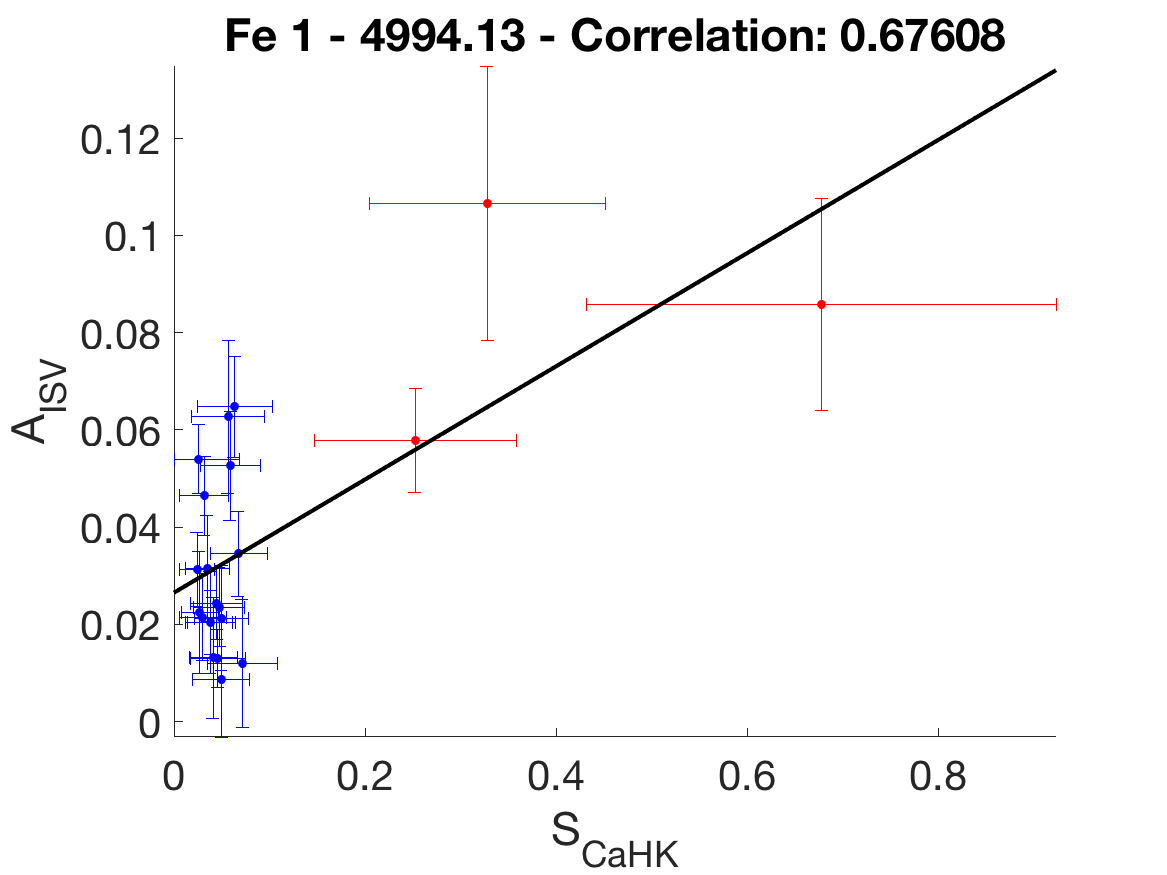
\includegraphics[width=0.5\textwidth]{CorrPlots/CaHK_2.png}}
    \subfloat[]{\label{figCa3}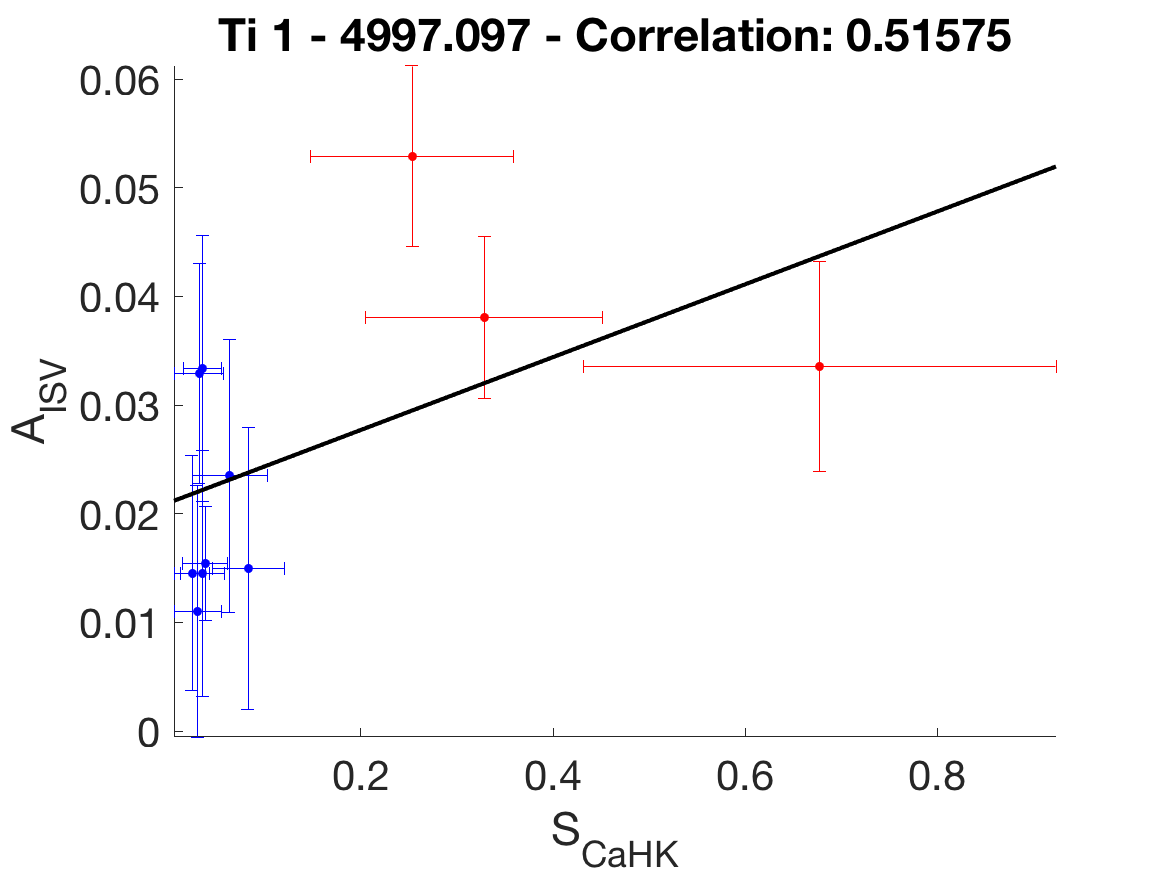
\includegraphics[width=0.5\textwidth]{CorrPlots/CaHK_3.png}}\\
    \subfloat[]{\label{figHa2}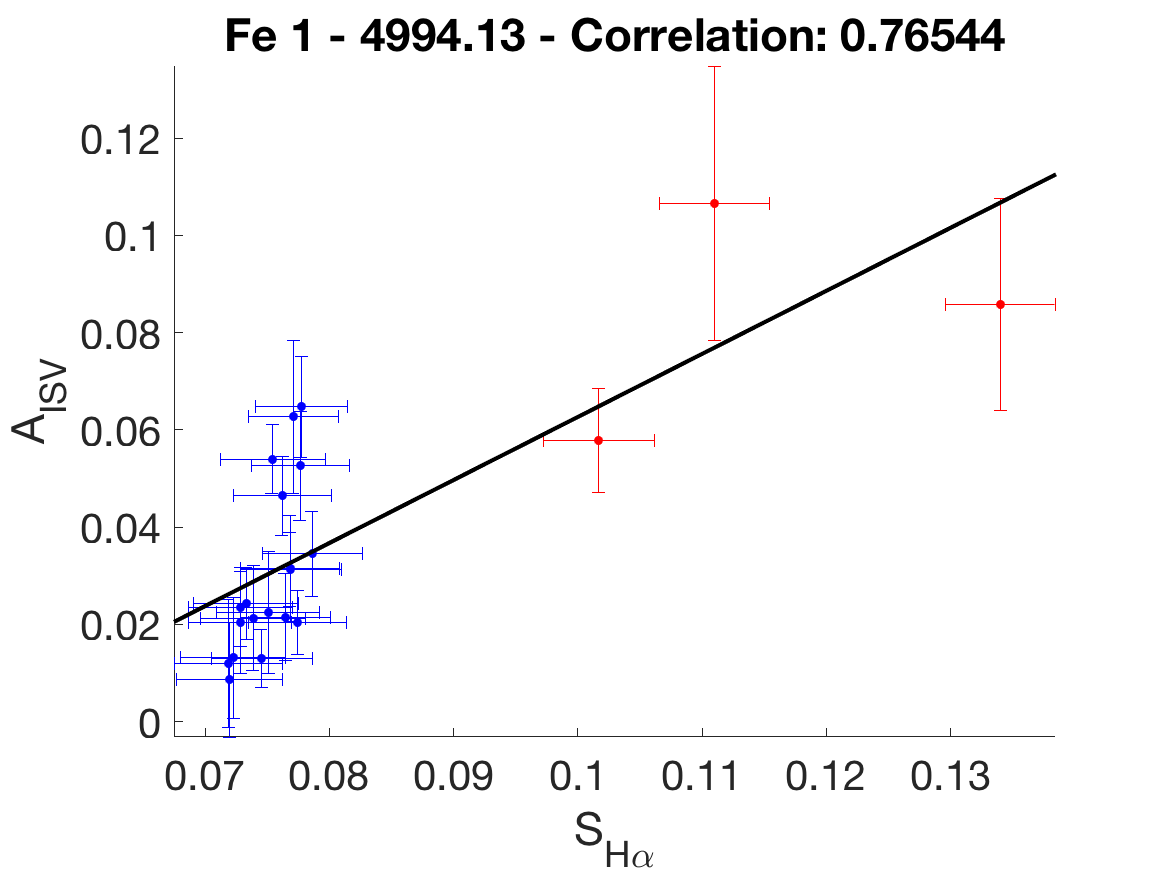
\includegraphics[width=0.5\textwidth]{CorrPlots/Halpha_2.png}}
    \subfloat[]{\label{figHa3}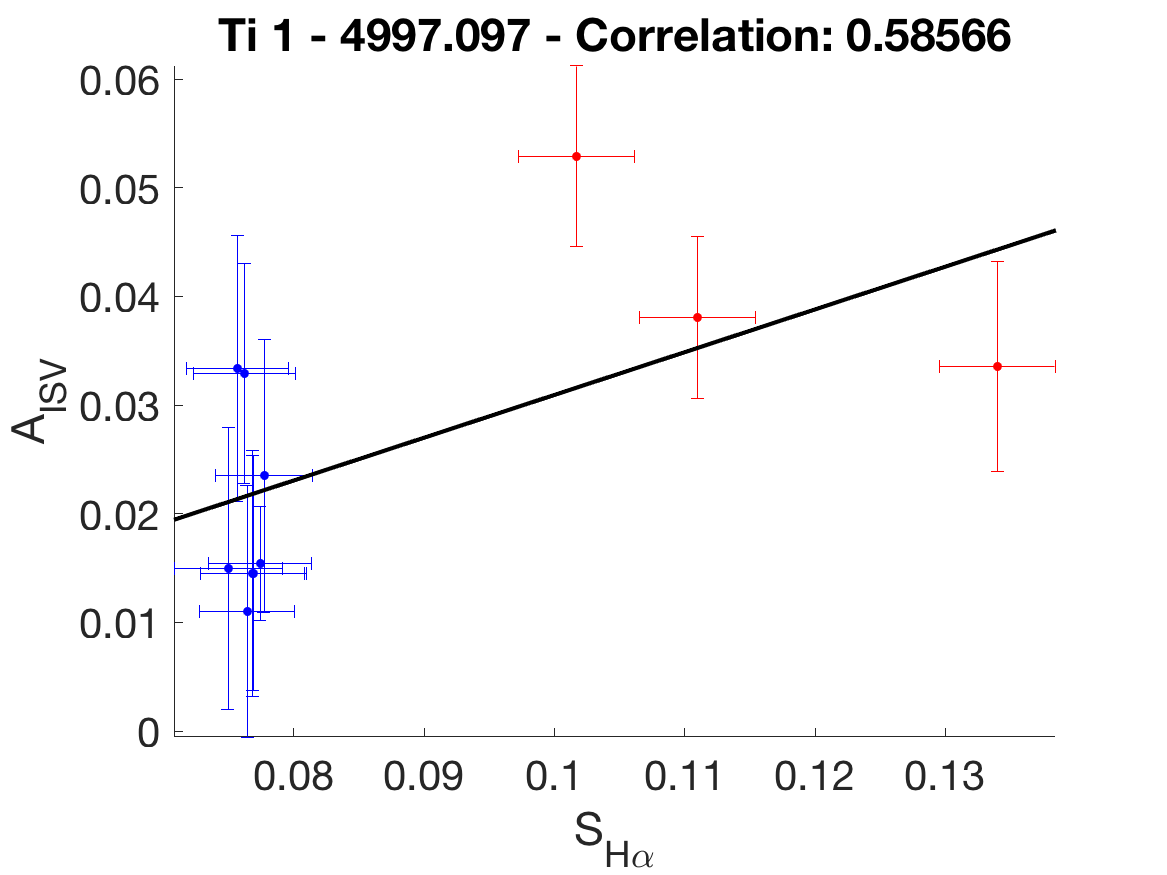
\includegraphics[width=0.5\textwidth]{CorrPlots/Halpha_3.png}}\\
    \subfloat[]{\label{figNa2}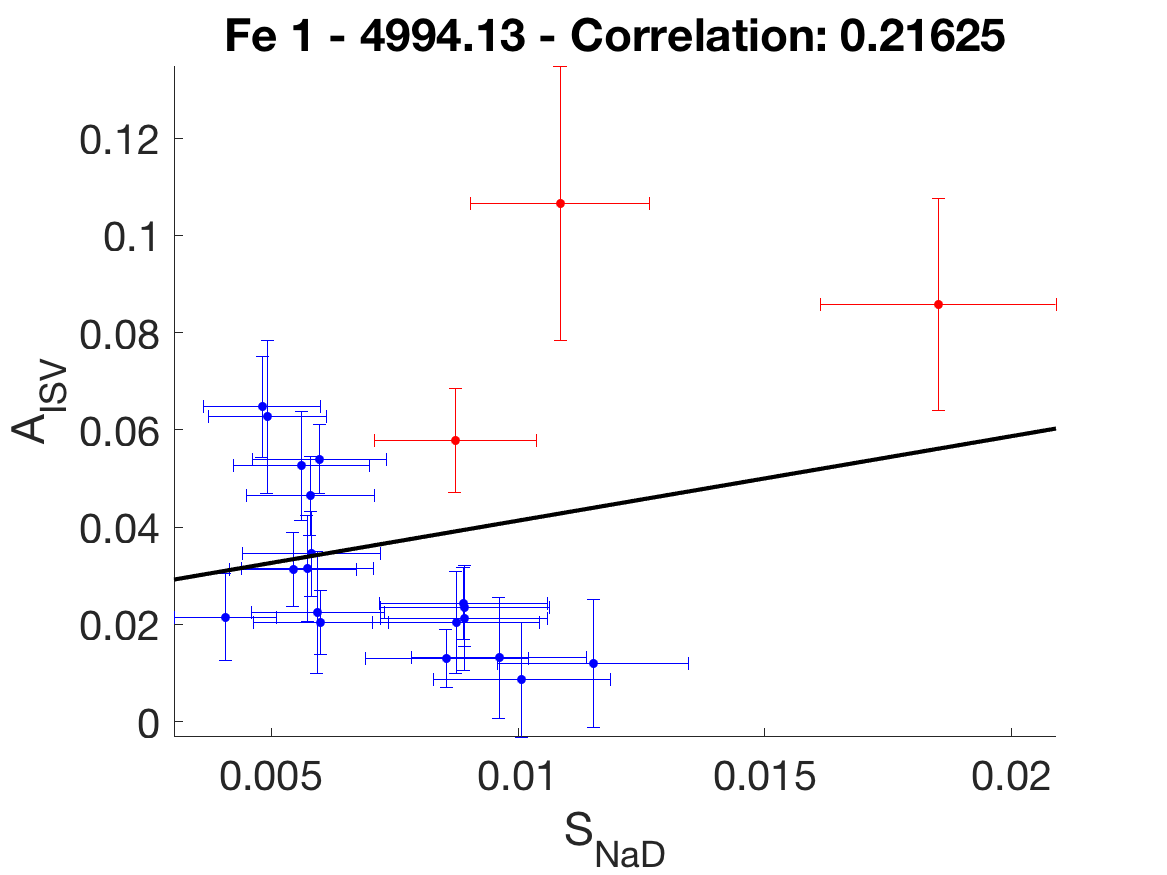
\includegraphics[width=0.5\textwidth]{CorrPlots/NaD_2.png}}
    \subfloat[]{\label{figNa3}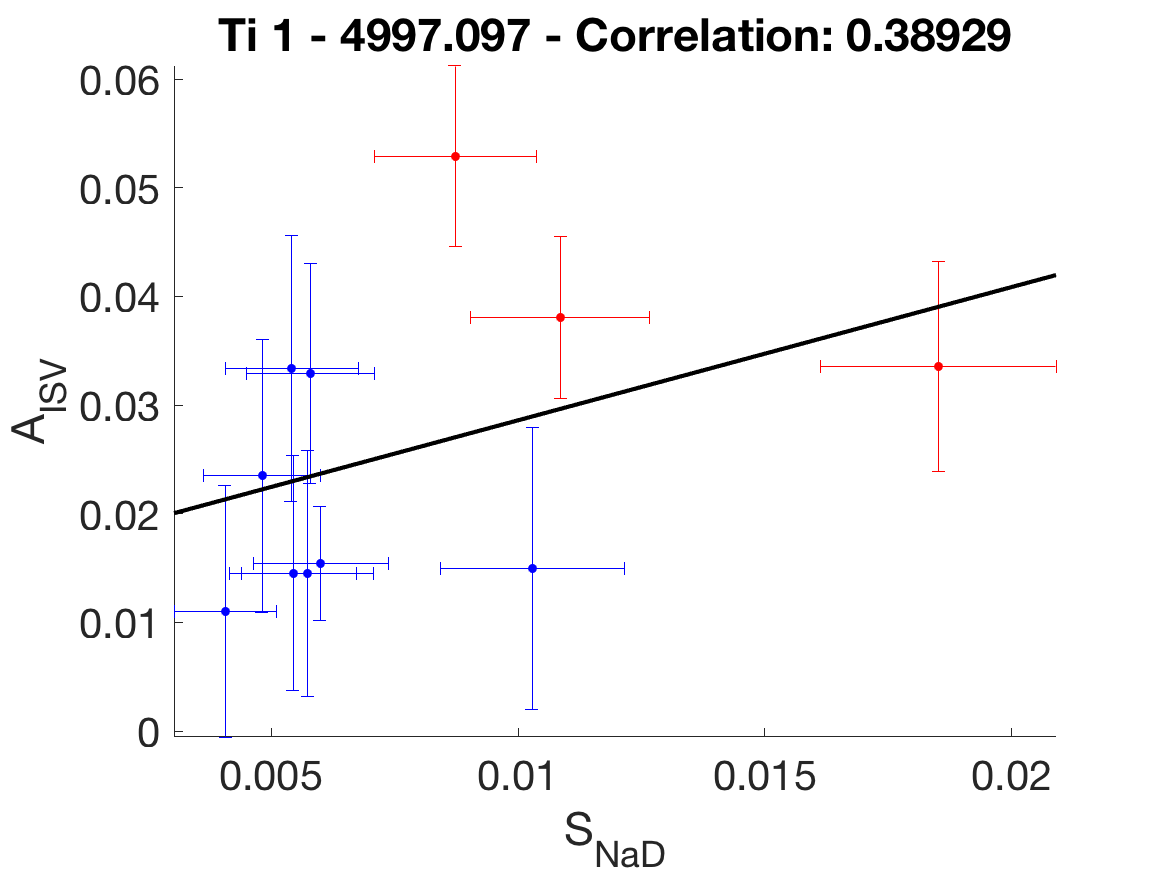
\includegraphics[width=0.5\textwidth]{CorrPlots/NaD_3.png}}\\
    \caption{}
    \label{figCorr1}
\end{figure}

\begin{figure}[!h]
    \centering
	\captionsetup{width=.8\textwidth}
    \subfloat[]{\label{figCa4}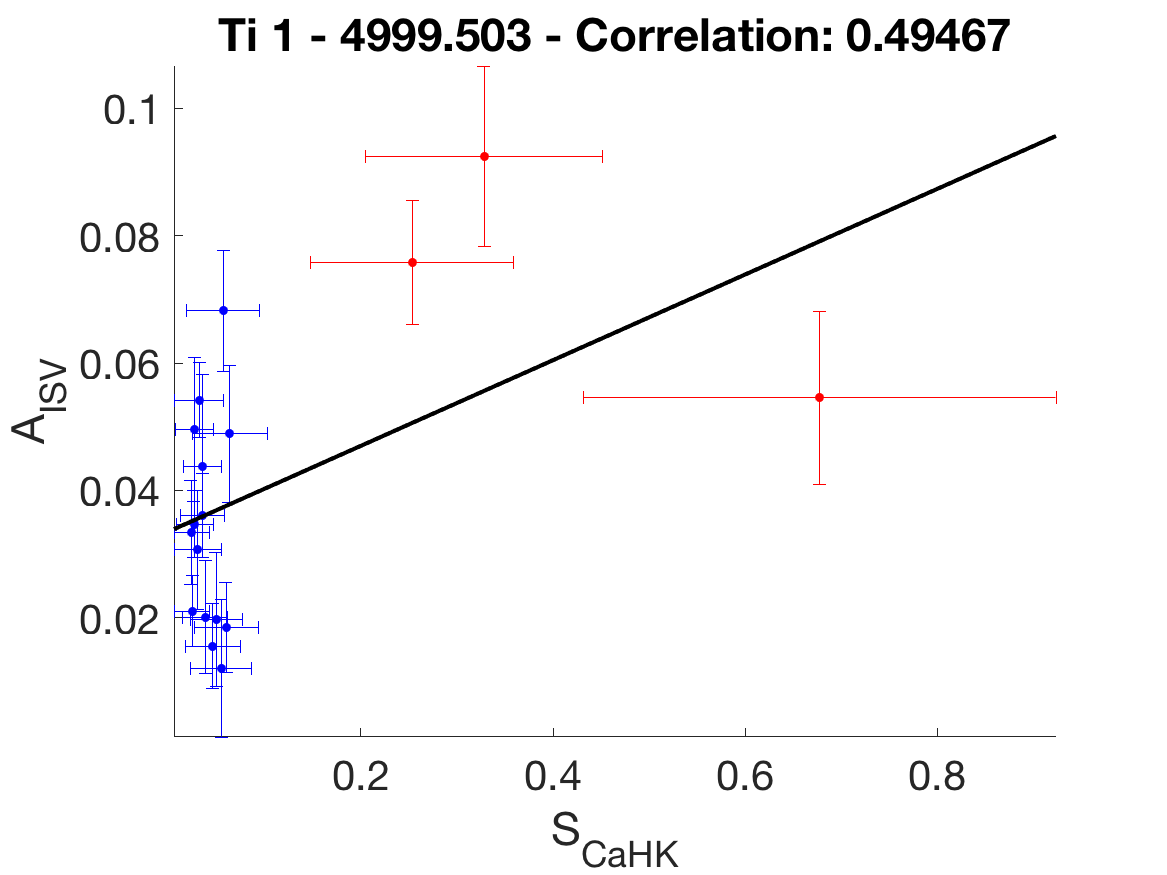
\includegraphics[width=0.5\textwidth]{CorrPlots/CaHK_4.png}}
    \subfloat[]{\label{figCa7}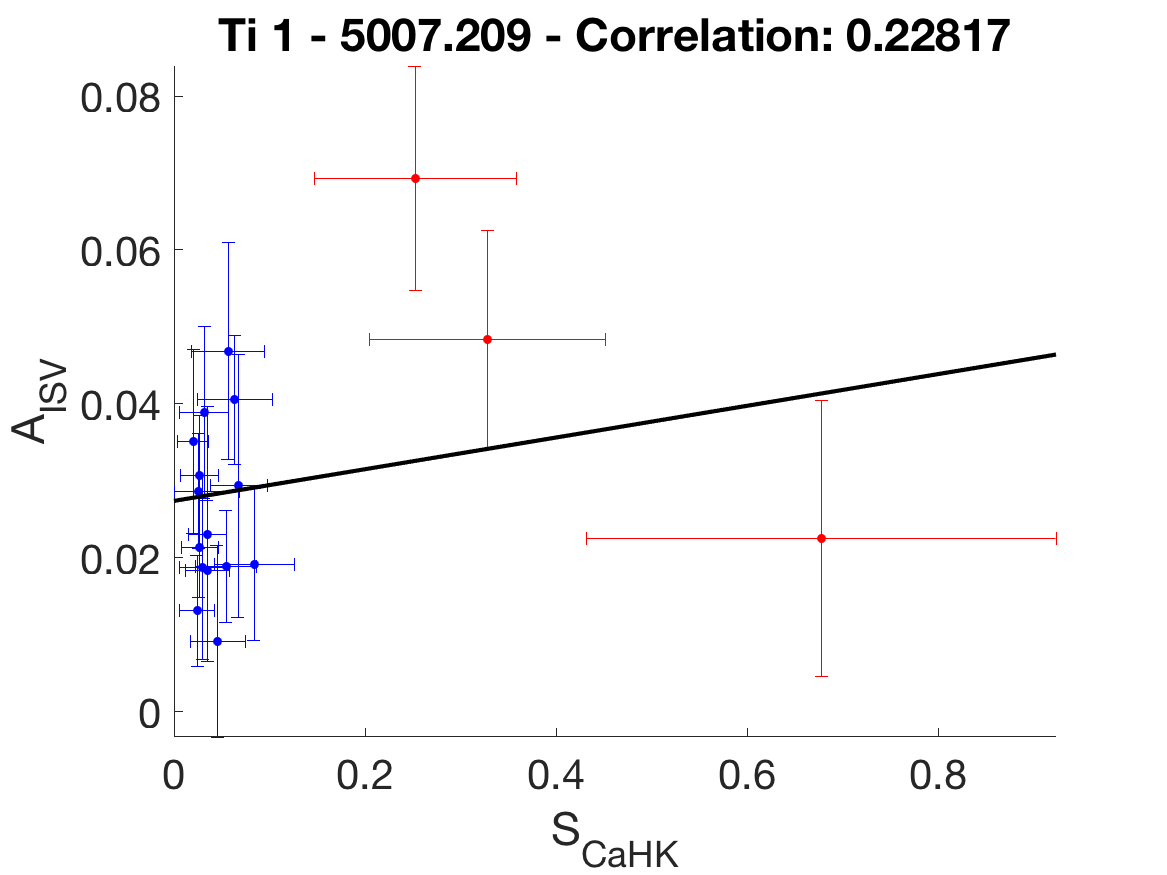
\includegraphics[width=0.5\textwidth]{CorrPlots/CaHK_7.png}}\\
    \subfloat[]{\label{figHa4}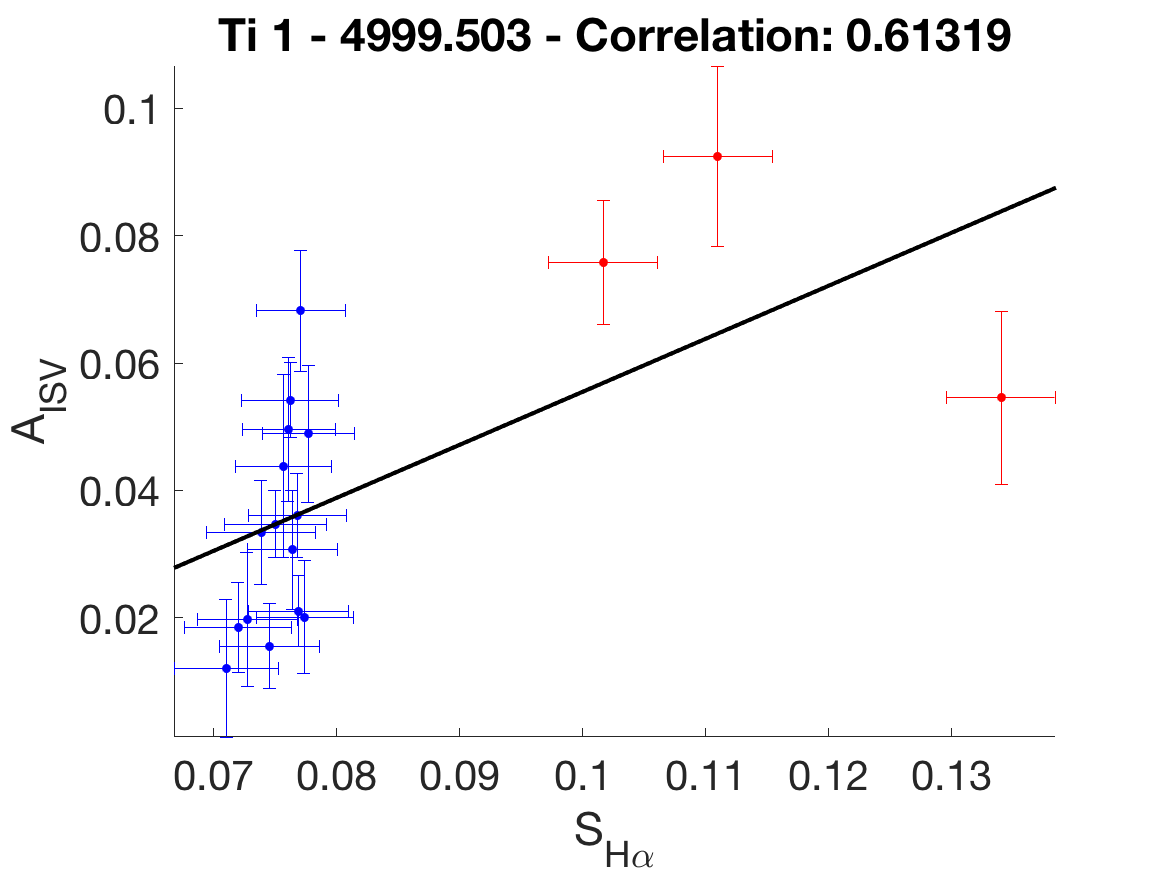
\includegraphics[width=0.5\textwidth]{CorrPlots/Halpha_4.png}}
    \subfloat[]{\label{figHa7}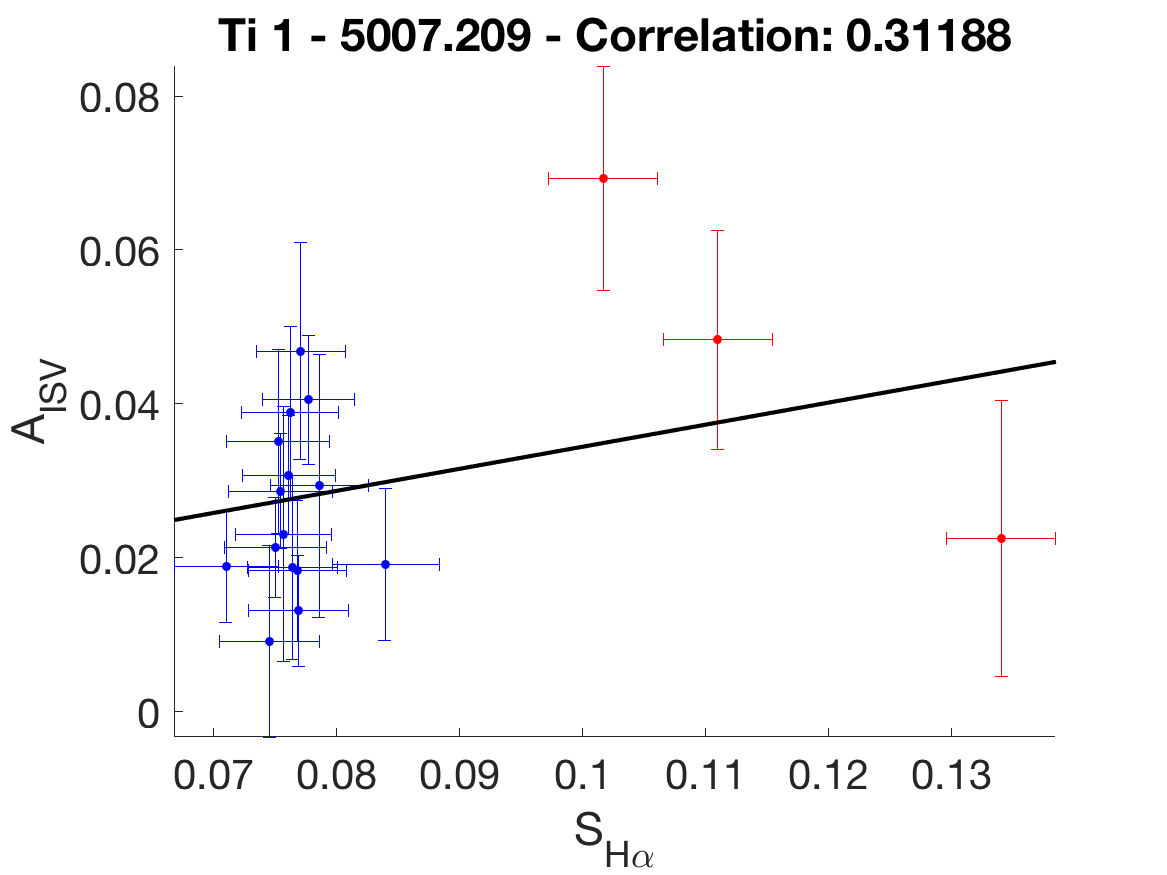
\includegraphics[width=0.5\textwidth]{CorrPlots/Halpha_7.png}}\\
    \subfloat[]{\label{figNa4}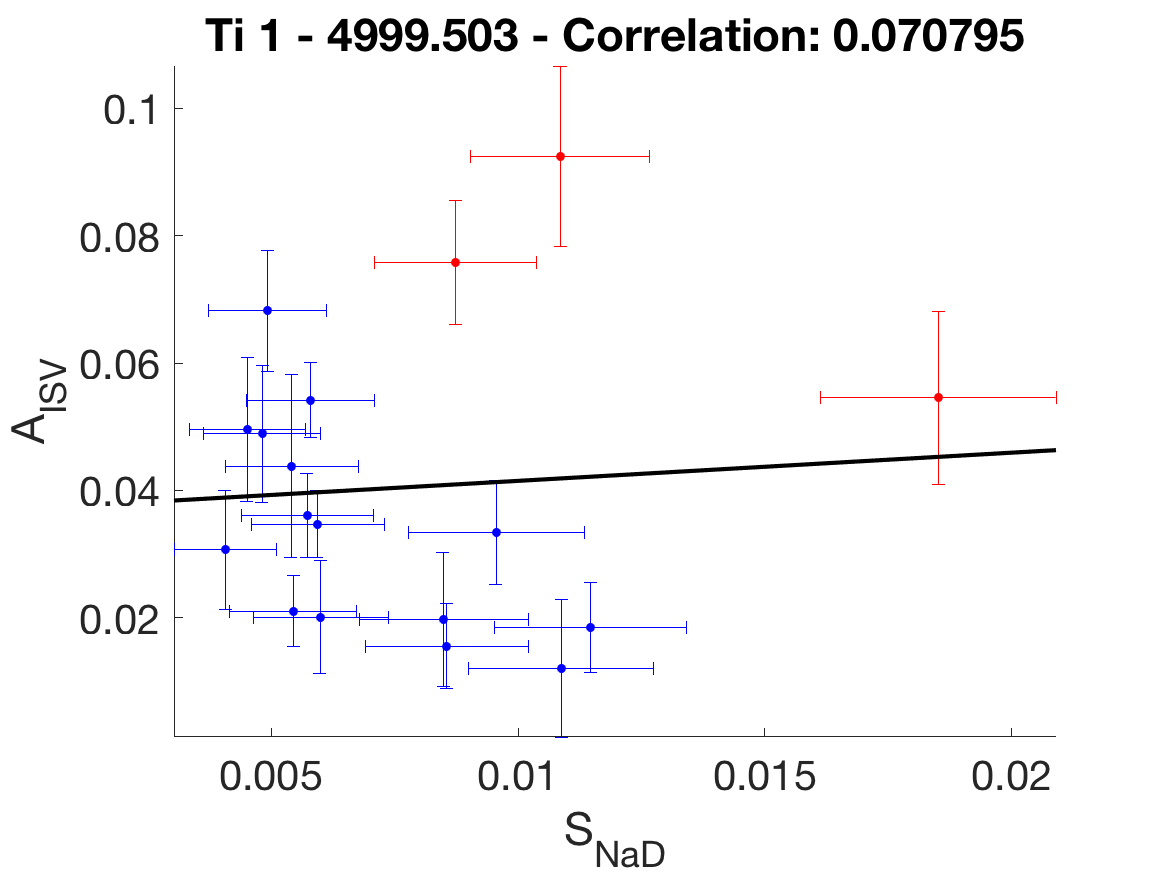
\includegraphics[width=0.5\textwidth]{CorrPlots/NaD_4.png}}
    \subfloat[]{\label{figNa7}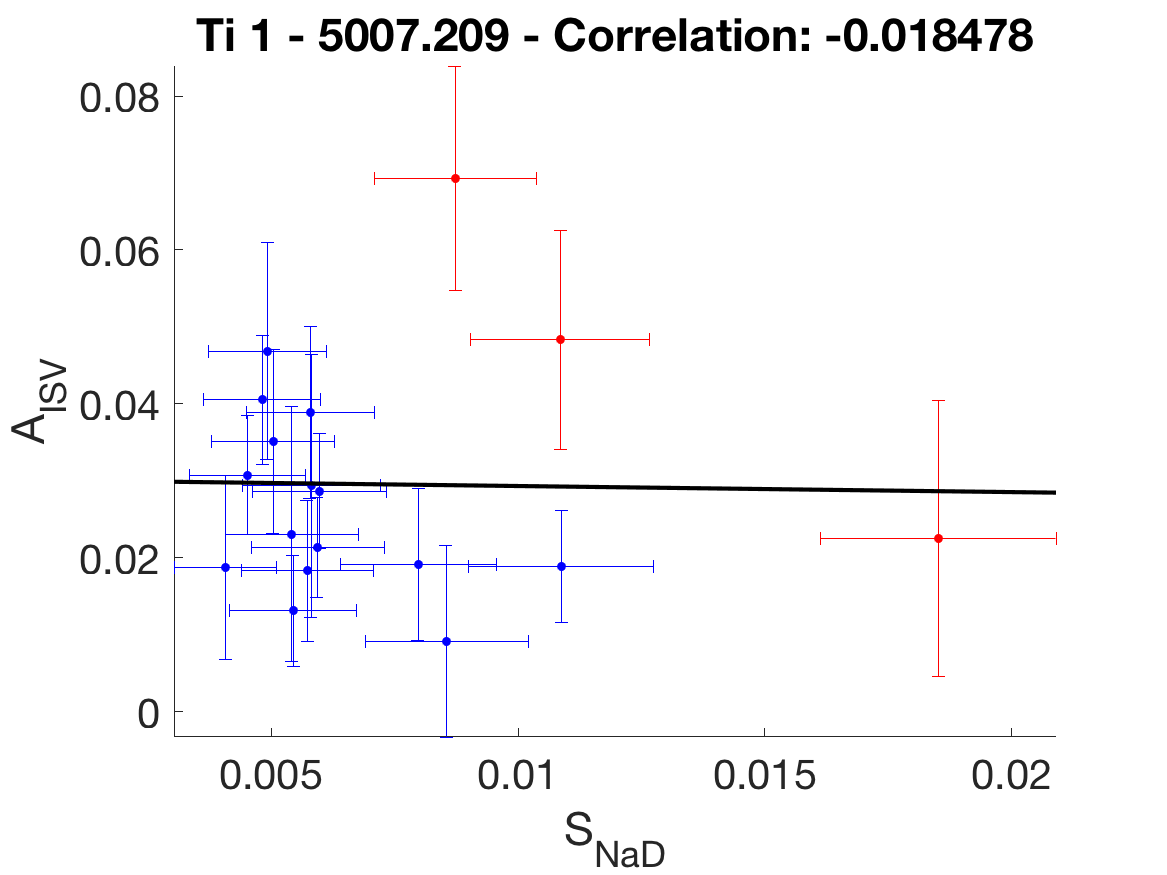
\includegraphics[width=0.5\textwidth]{CorrPlots/NaD_7.png}}\\
    \caption{}
    \label{figCorr2}
\end{figure}

\begin{figure}[!h]
    \centering
	\captionsetup{width=.8\textwidth}
    \subfloat[]{\label{figCa9}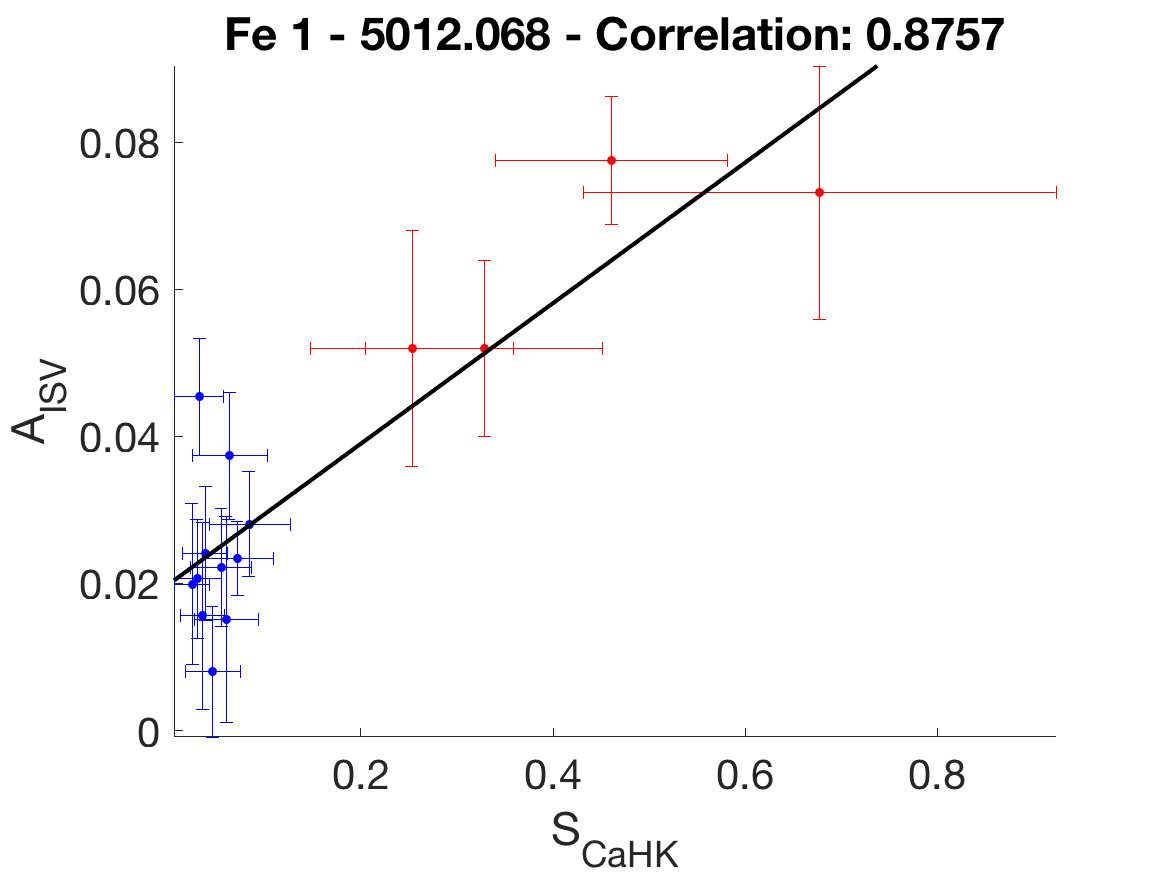
\includegraphics[width=0.5\textwidth]{CorrPlots/CaHK_9.png}}
    \subfloat[]{\label{figCa12}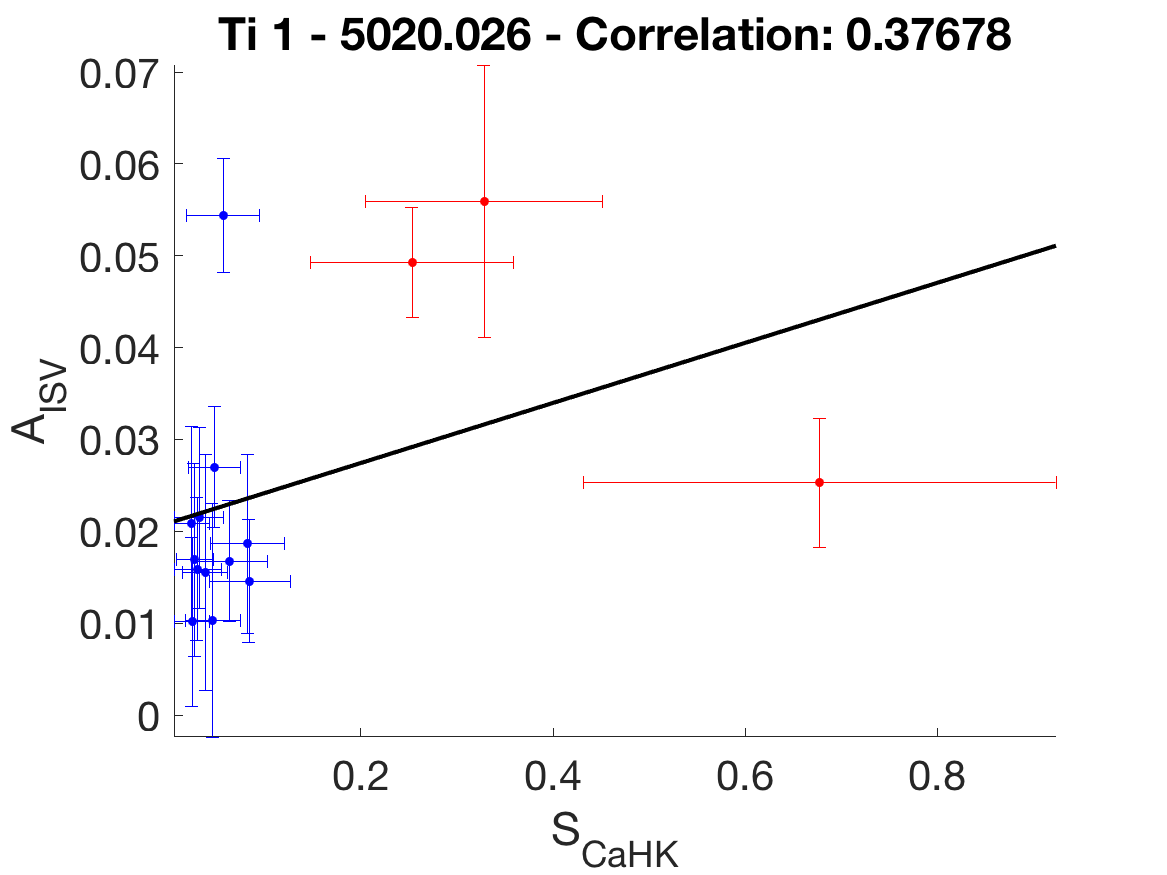
\includegraphics[width=0.5\textwidth]{CorrPlots/CaHK_12.png}}\\
    \subfloat[]{\label{figHa9}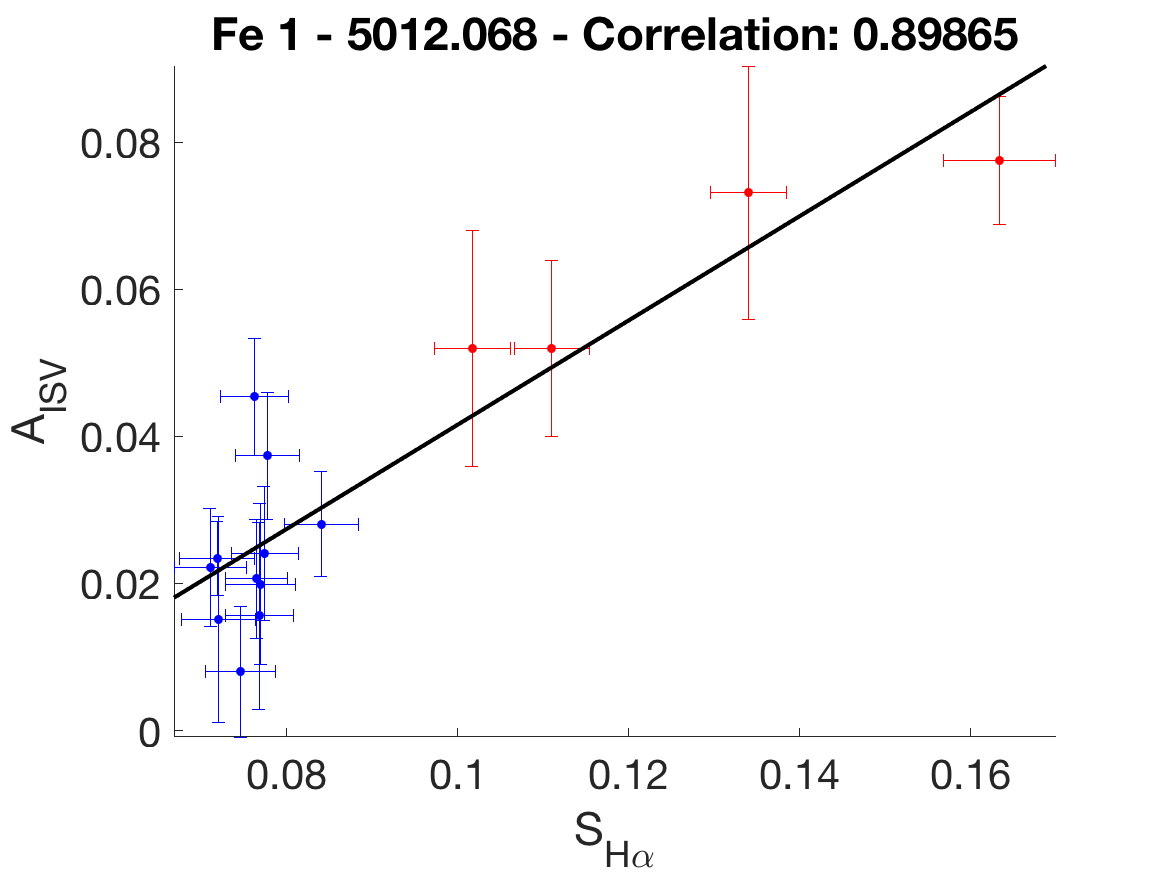
\includegraphics[width=0.5\textwidth]{CorrPlots/Halpha_9.png}}
    \subfloat[]{\label{figHa12}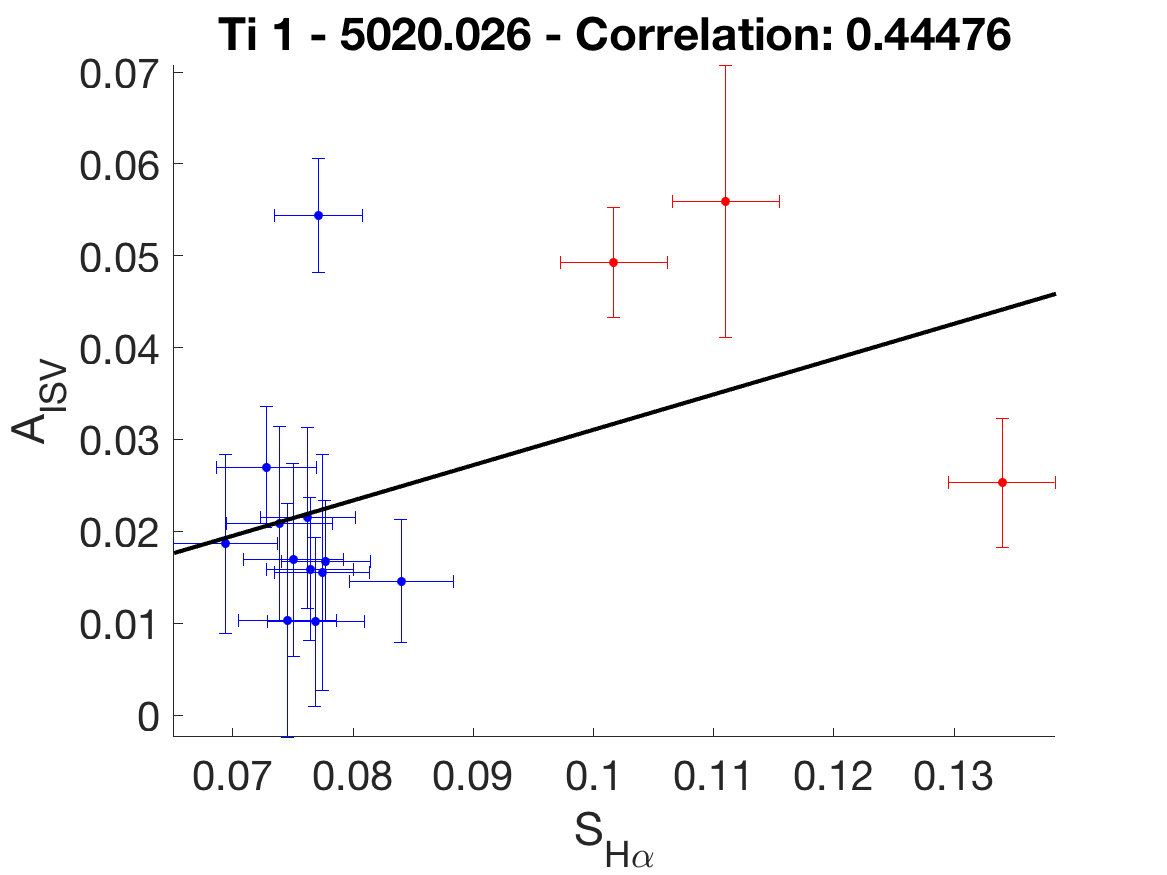
\includegraphics[width=0.5\textwidth]{CorrPlots/Halpha_12.png}}\\
    \subfloat[]{\label{figNa9}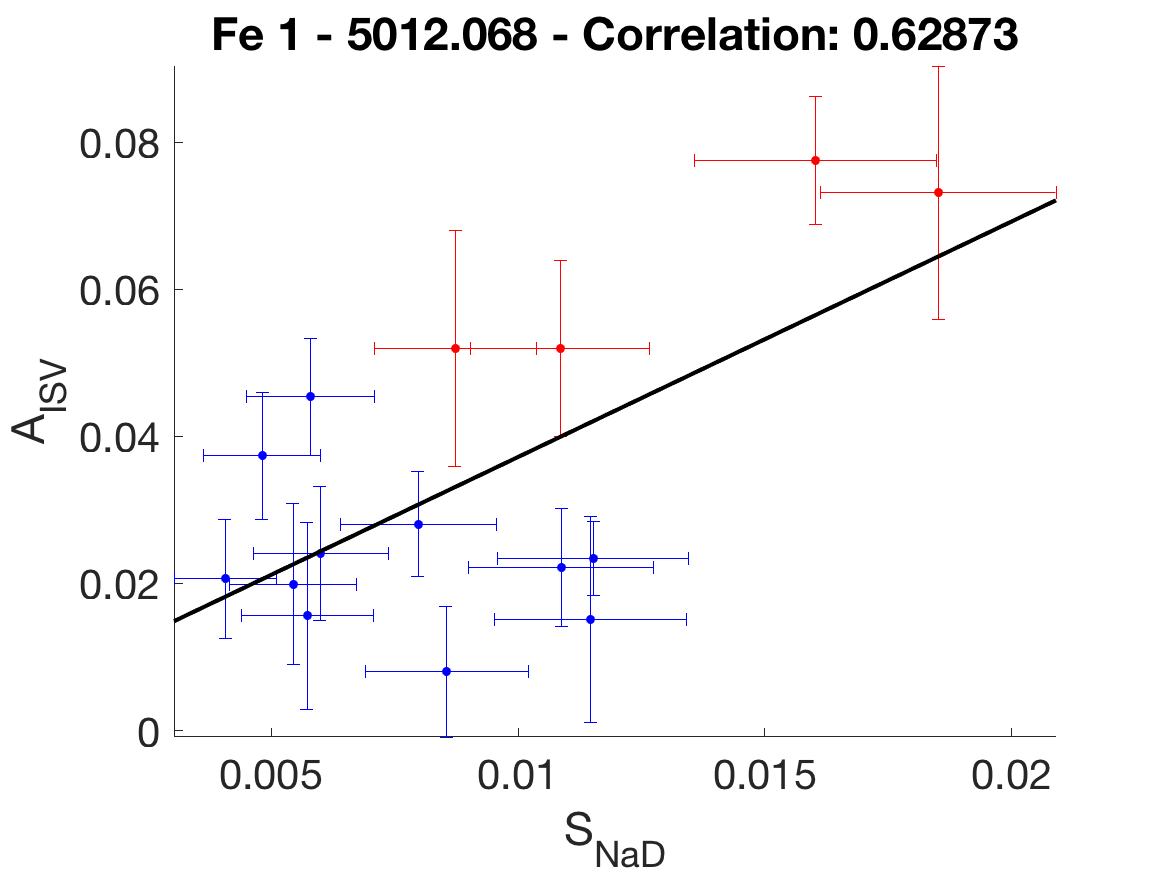
\includegraphics[width=0.5\textwidth]{CorrPlots/NaD_9.png}}
    \subfloat[]{\label{figNa12}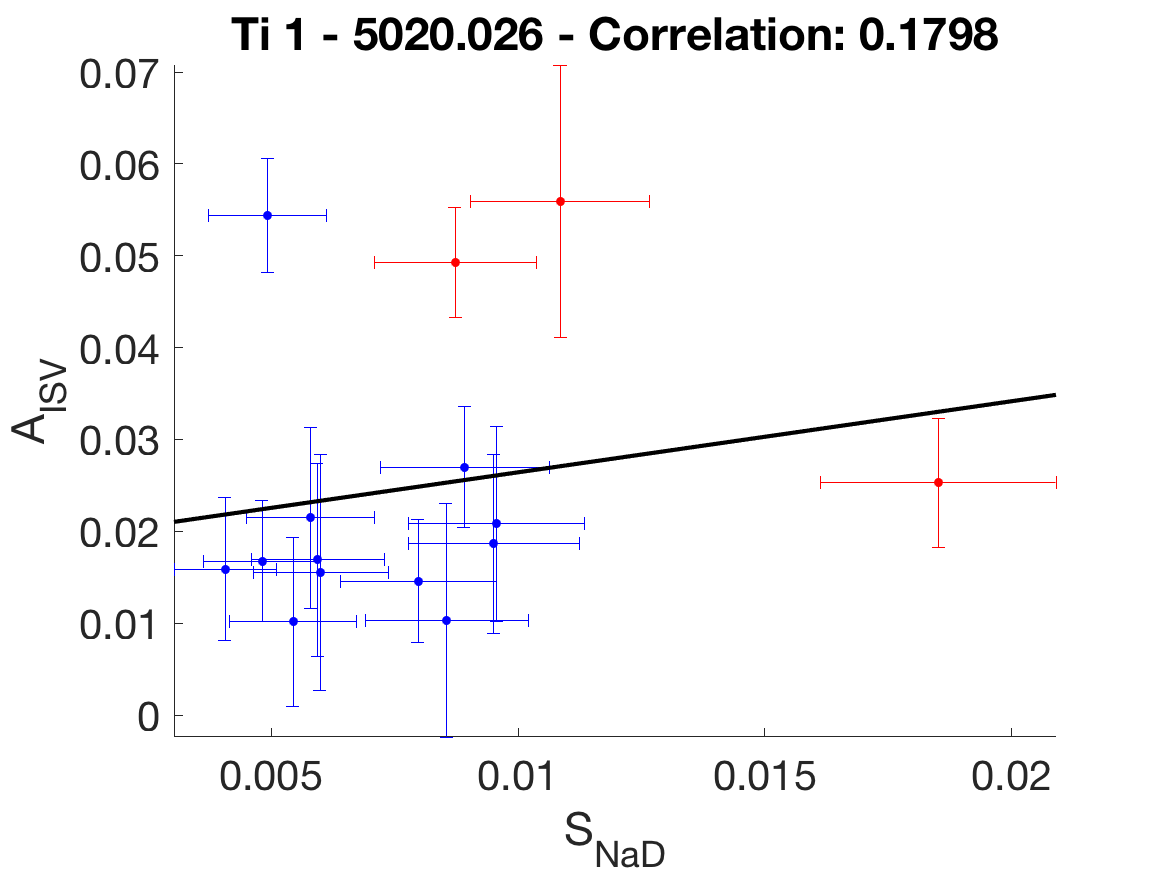
\includegraphics[width=0.5\textwidth]{CorrPlots/NaD_12.png}}\\
    \caption{}
    \label{figCorr3}
\end{figure}

\begin{figure}[!h]
    \centering
	\captionsetup{width=.8\textwidth}
    \subfloat[]{\label{figCa14}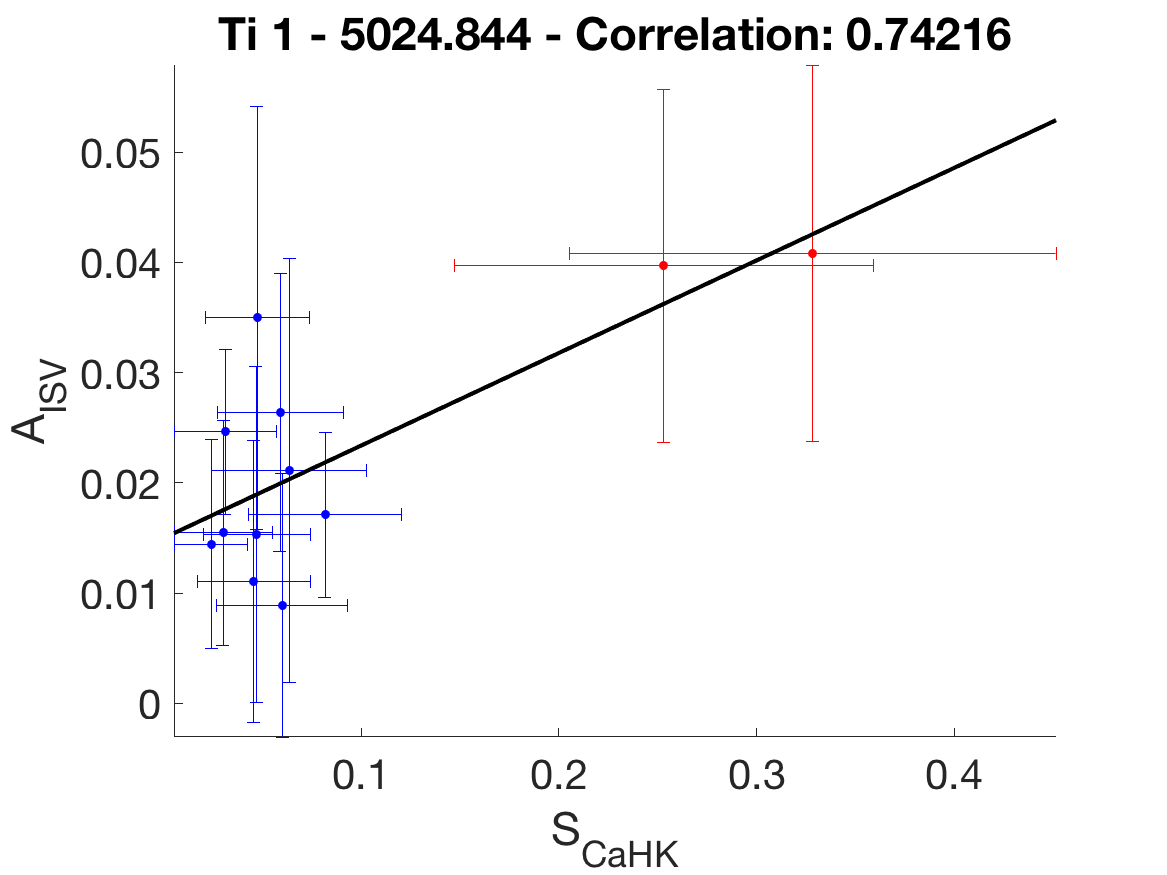
\includegraphics[width=0.5\textwidth]{CorrPlots/CaHK_14.png}}
    \subfloat[]{\label{figCa17}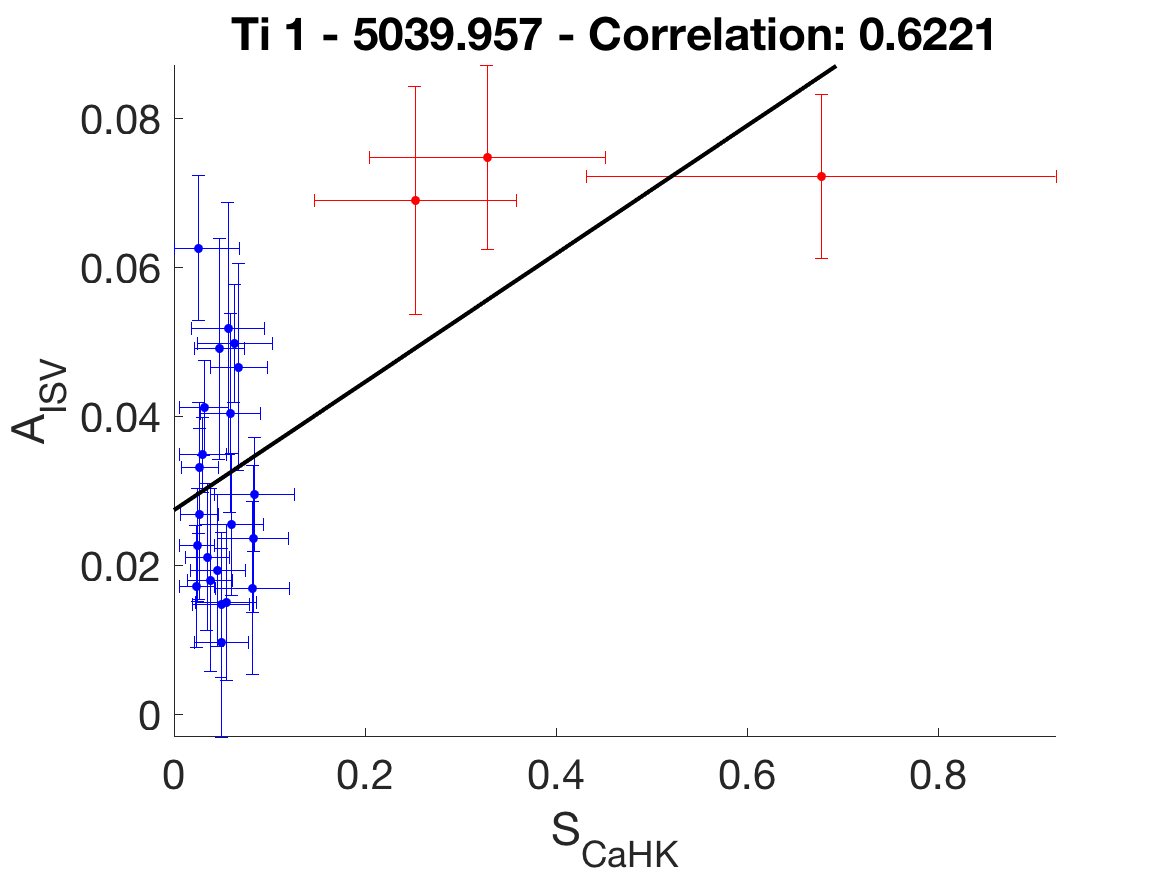
\includegraphics[width=0.5\textwidth]{CorrPlots/CaHK_17.png}}\\
    \subfloat[]{\label{figHa14}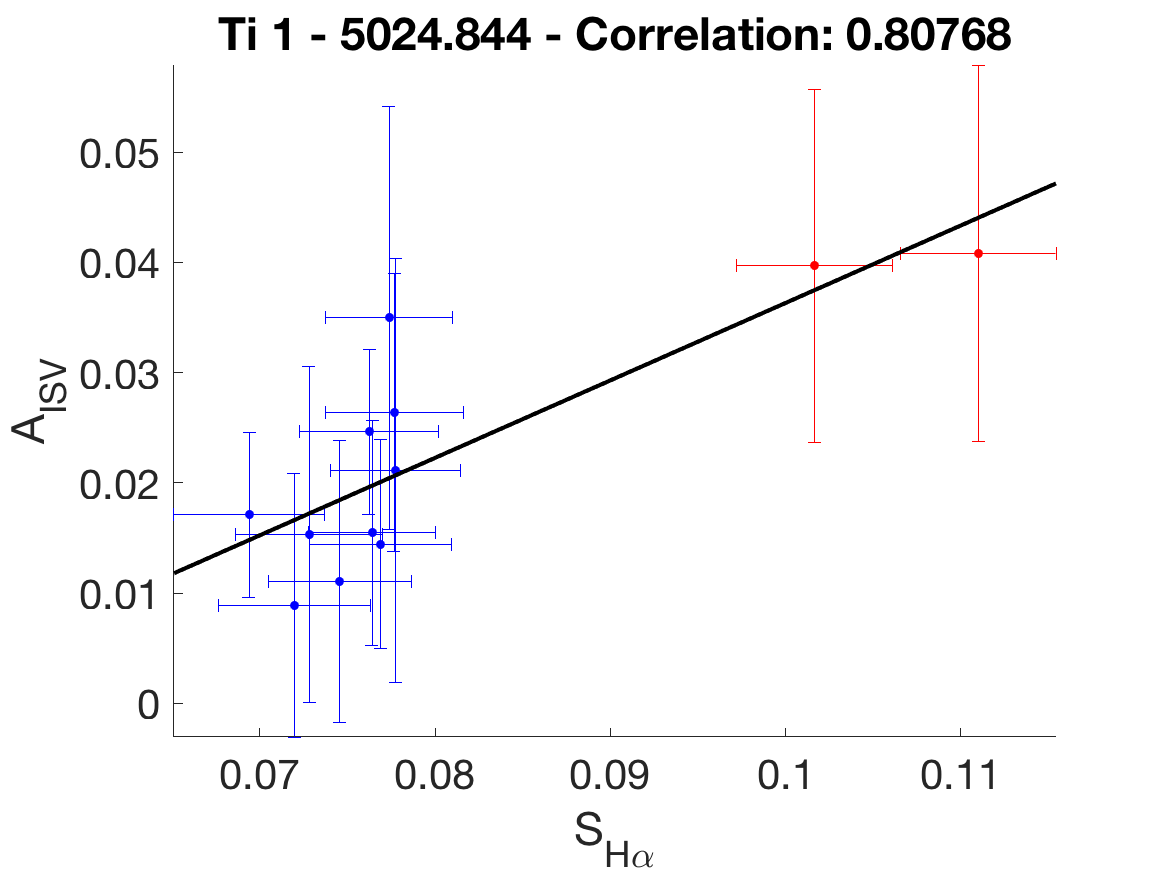
\includegraphics[width=0.5\textwidth]{CorrPlots/Halpha_14.png}}
    \subfloat[]{\label{figHa17}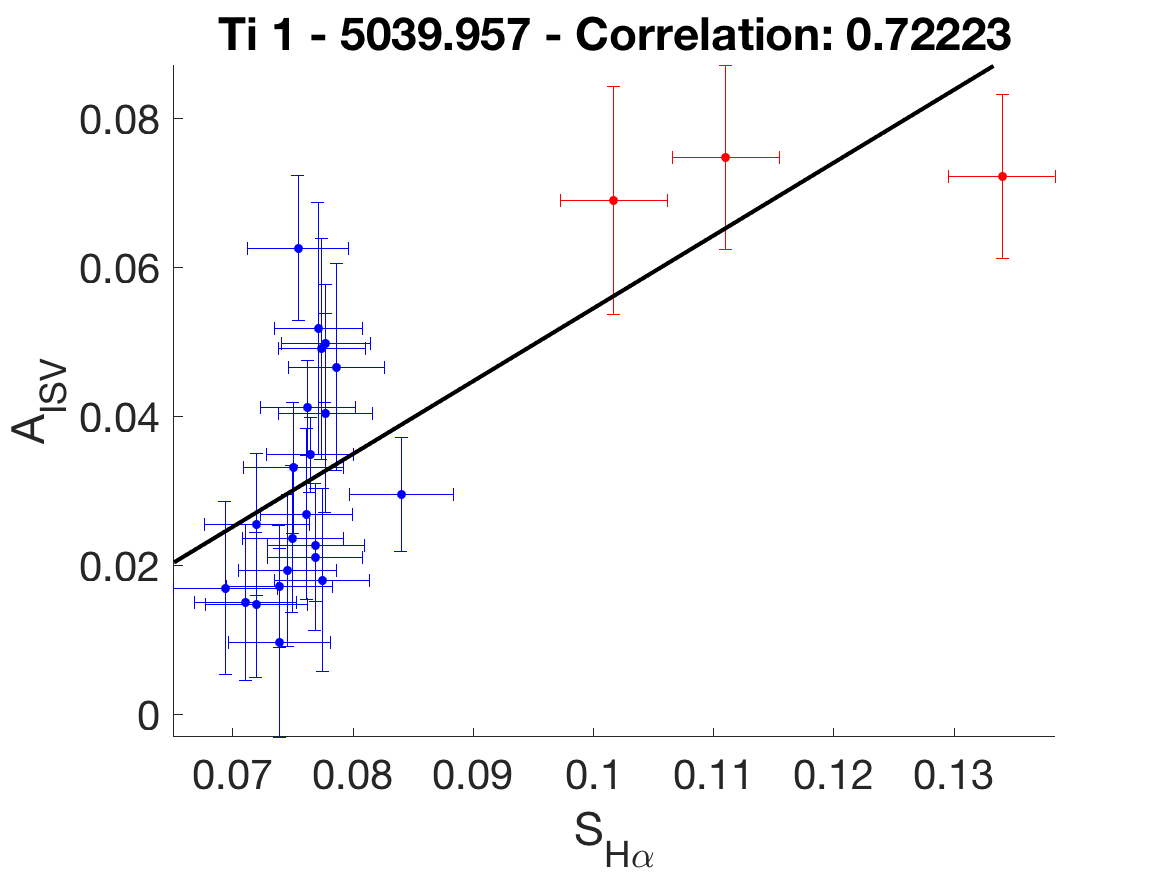
\includegraphics[width=0.5\textwidth]{CorrPlots/Halpha_17.png}}\\
    \subfloat[]{\label{figNa14}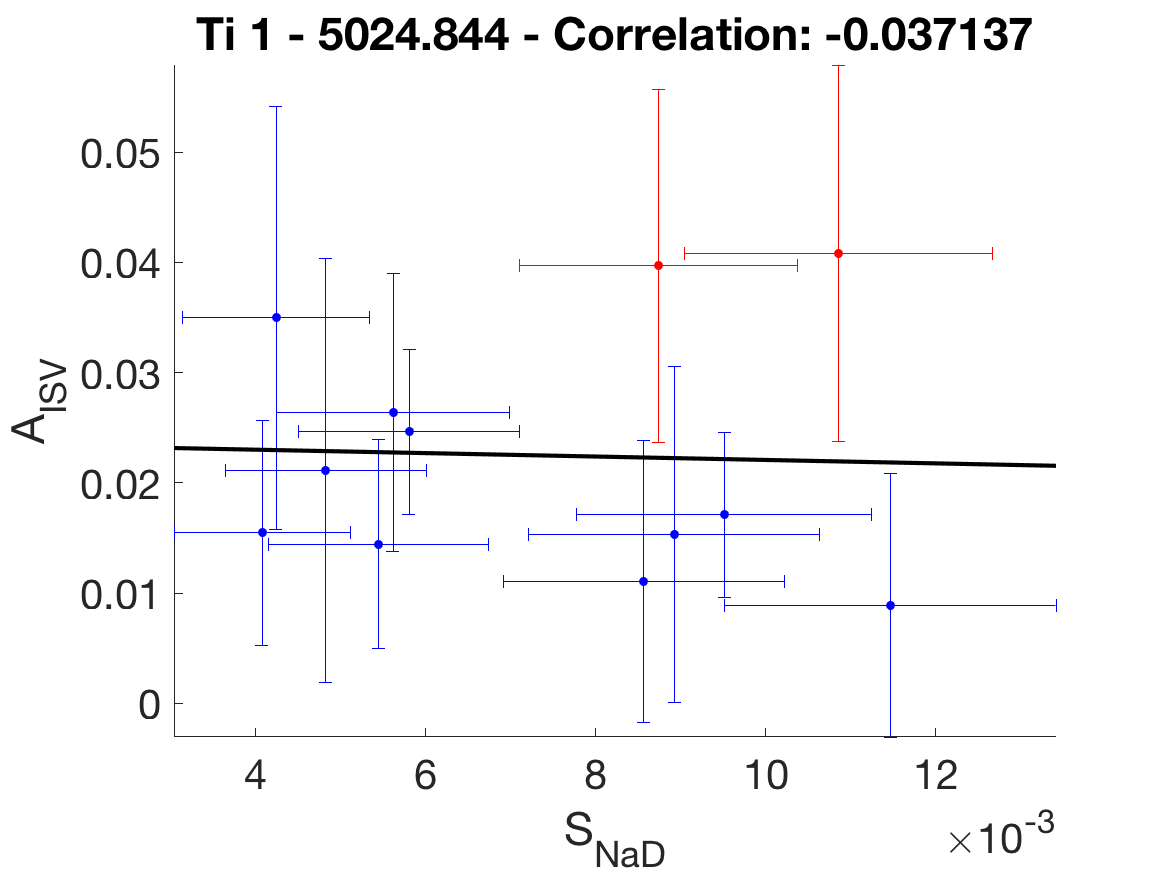
\includegraphics[width=0.5\textwidth]{CorrPlots/NaD_14.png}}
    \subfloat[]{\label{figNa17}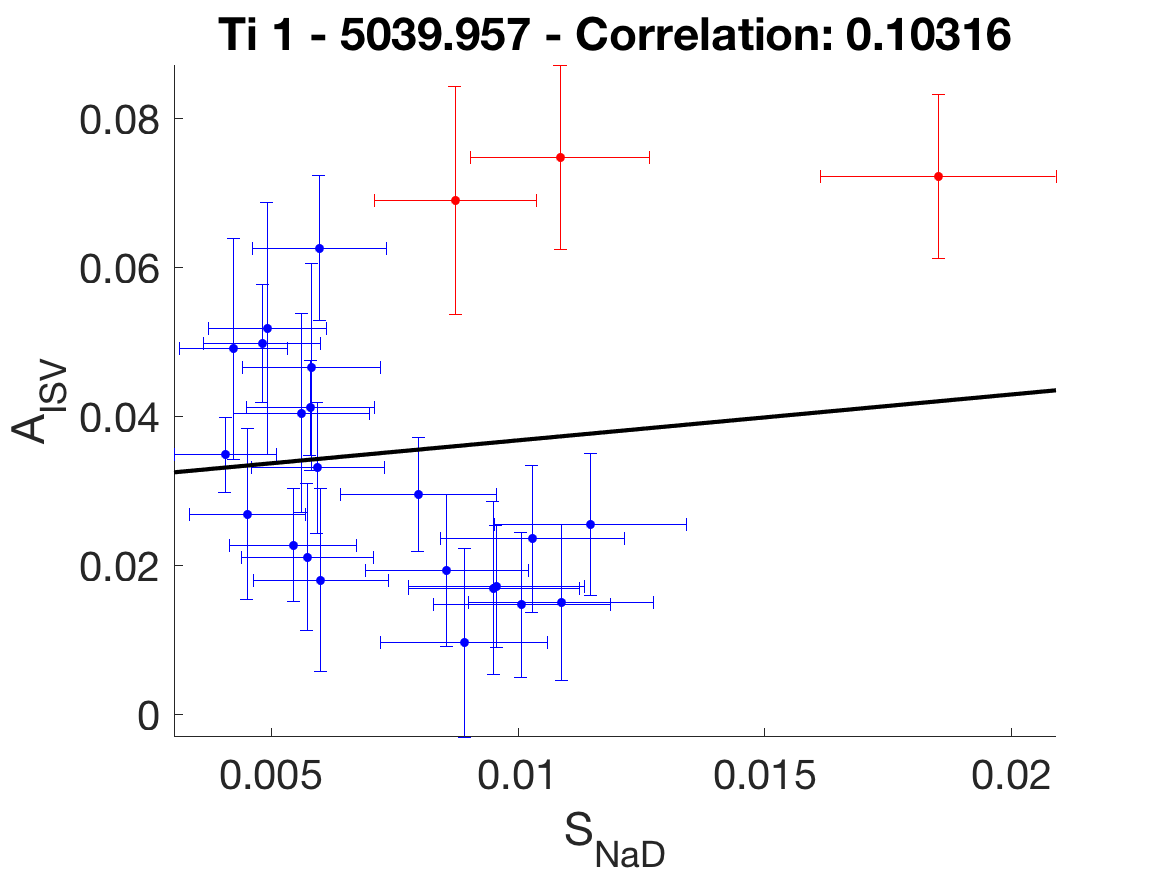
\includegraphics[width=0.5\textwidth]{CorrPlots/NaD_17.png}}\\
    \caption{}
    \label{figCorr4}
\end{figure}

\begin{figure}[!h]
    \centering
	\captionsetup{width=.8\textwidth}
    \subfloat[]{\label{figCa18}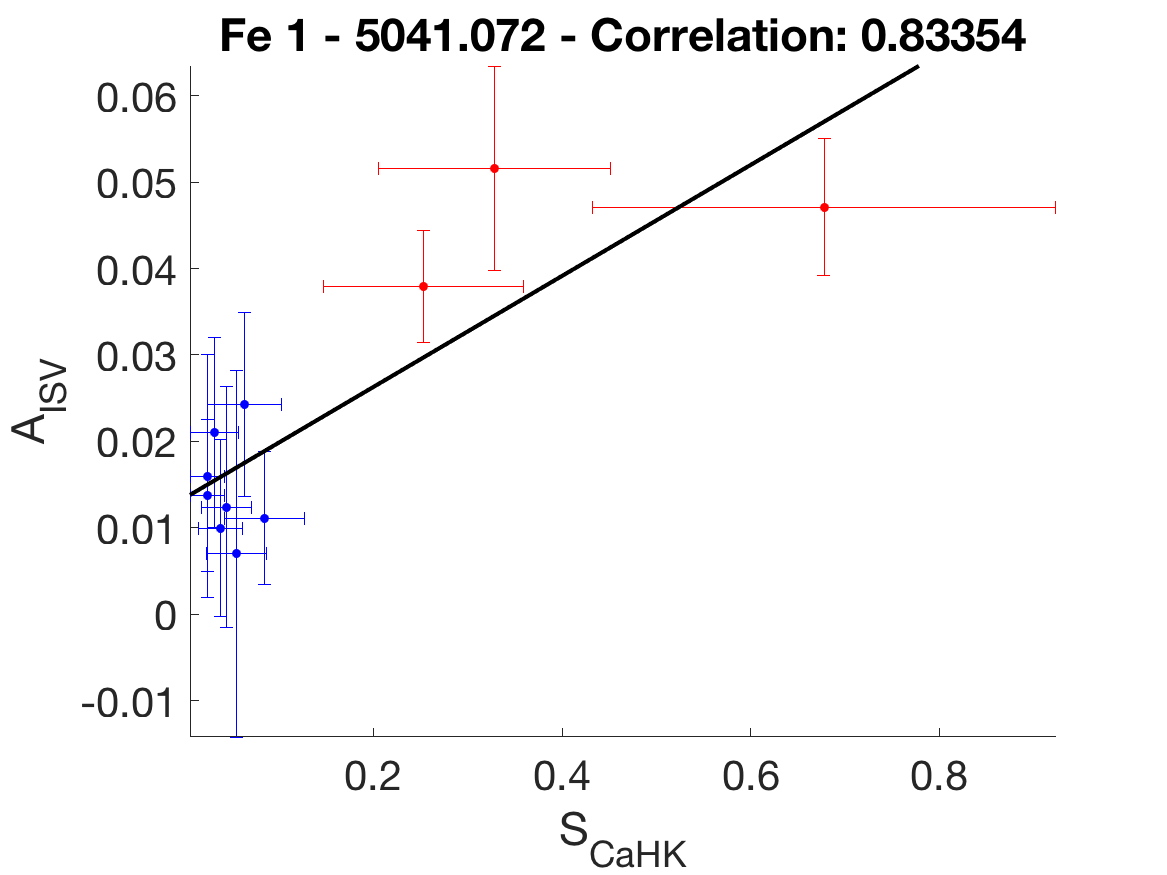
\includegraphics[width=0.5\textwidth]{CorrPlots/CaHK_18.png}}
    \subfloat[]{\label{figCa20}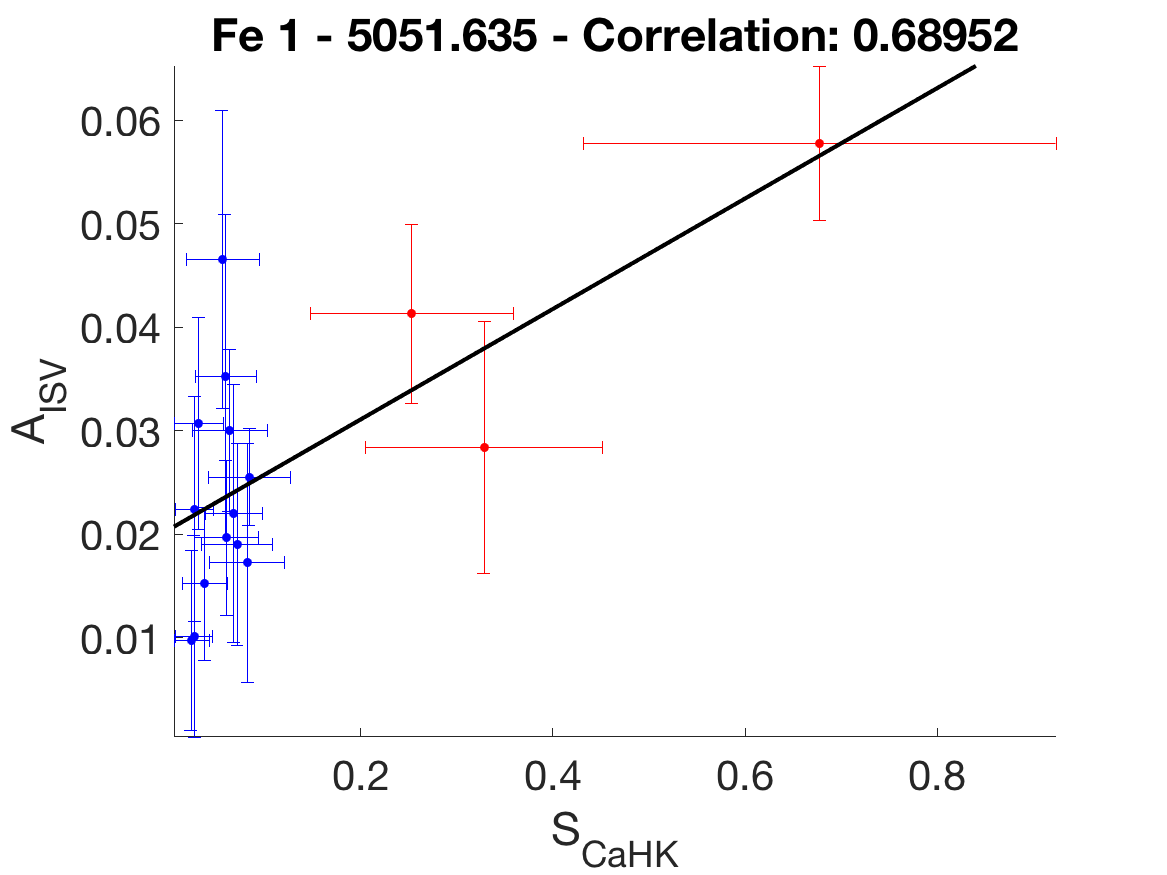
\includegraphics[width=0.5\textwidth]{CorrPlots/CaHK_20.png}}\\
    \subfloat[]{\label{figHa18}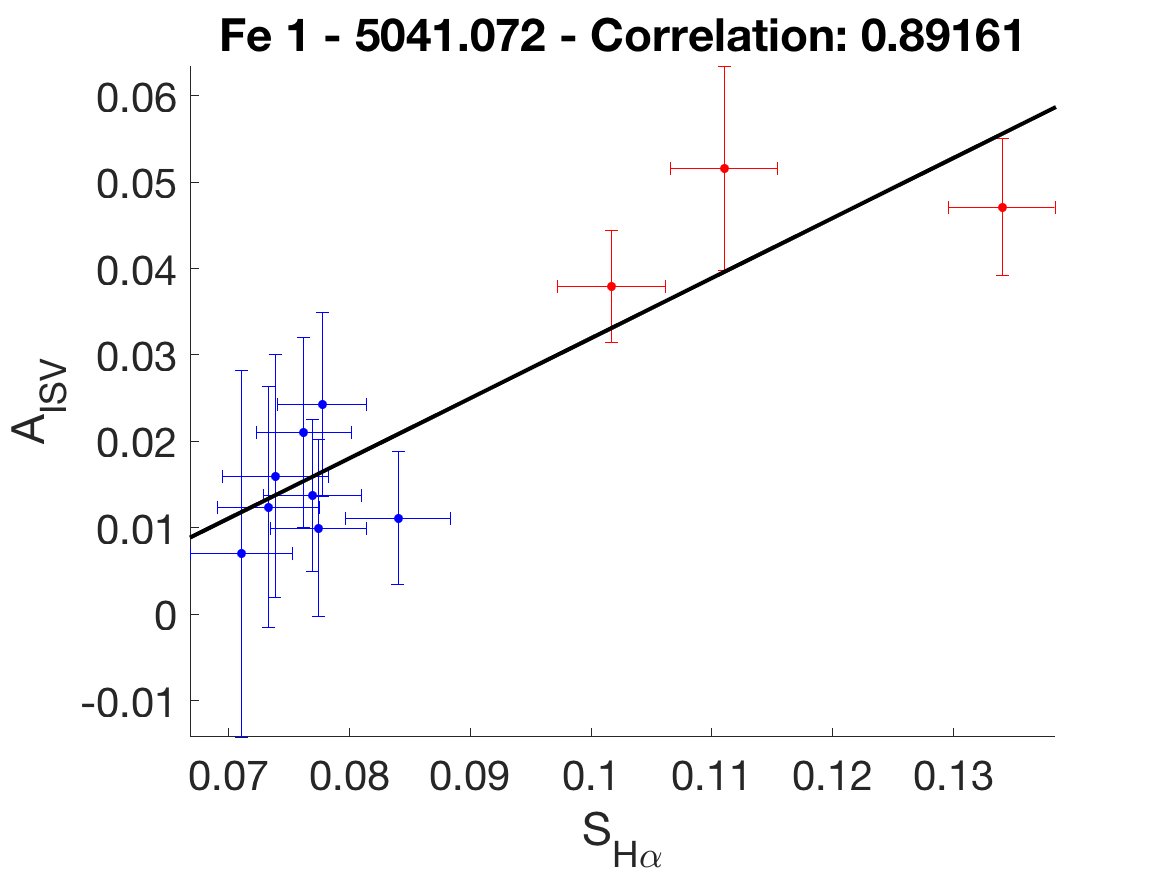
\includegraphics[width=0.5\textwidth]{CorrPlots/Halpha_18.png}}
    \subfloat[]{\label{figHa20}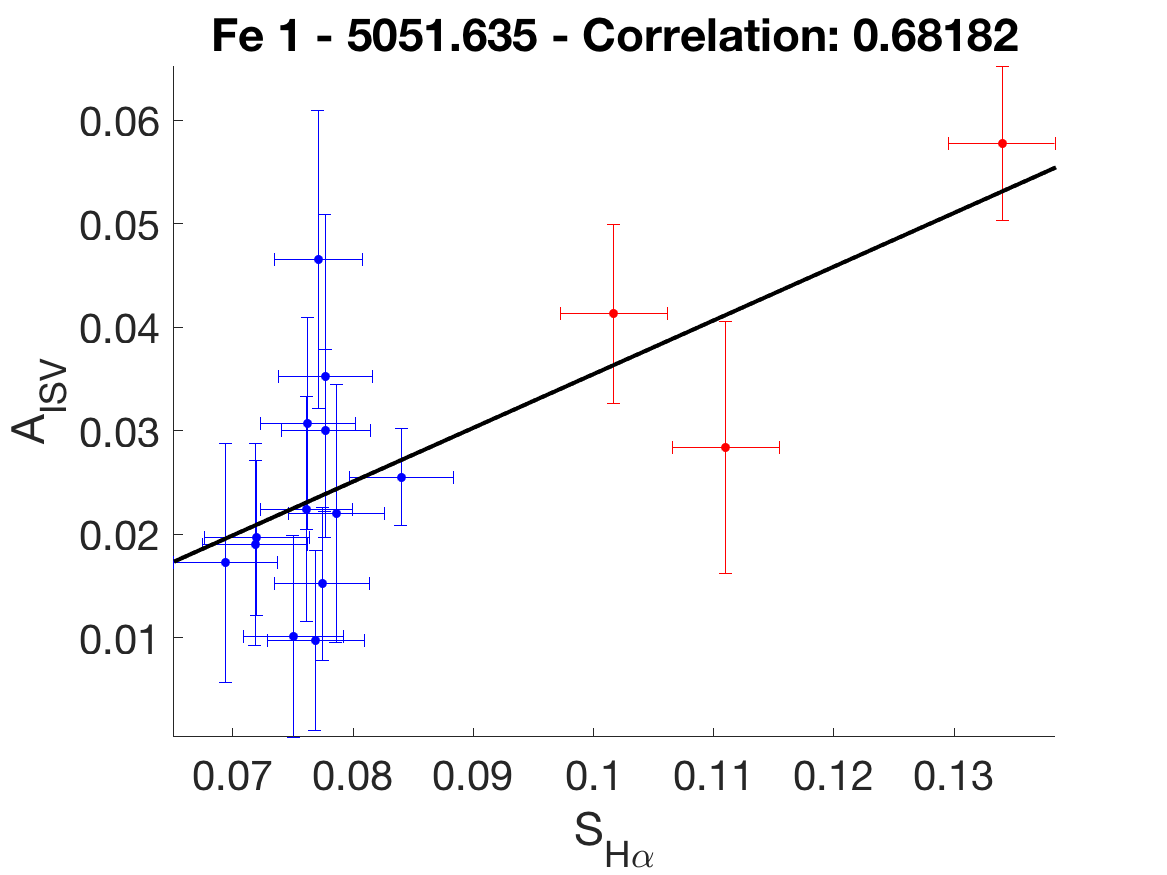
\includegraphics[width=0.5\textwidth]{CorrPlots/Halpha_20.png}}\\
    \subfloat[]{\label{figNa18}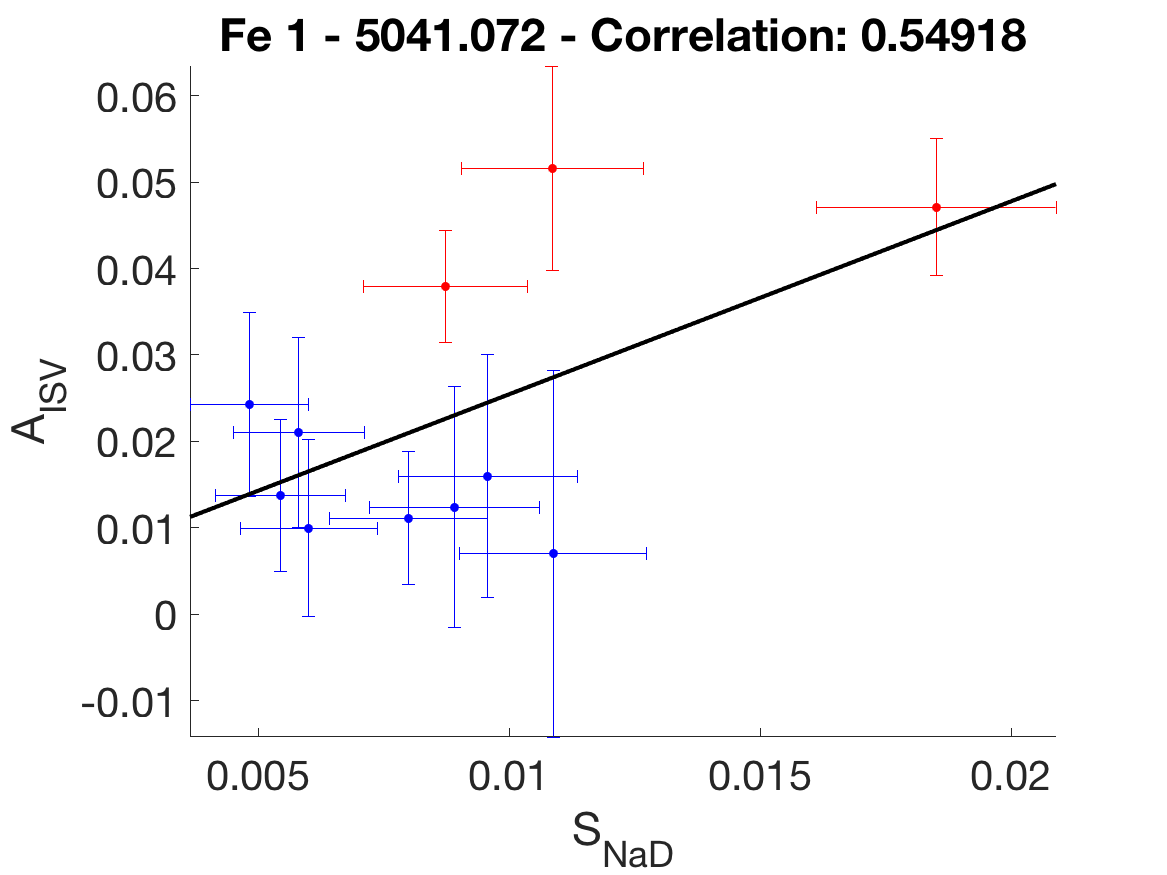
\includegraphics[width=0.5\textwidth]{CorrPlots/NaD_18.png}}
    \subfloat[]{\label{figNa20}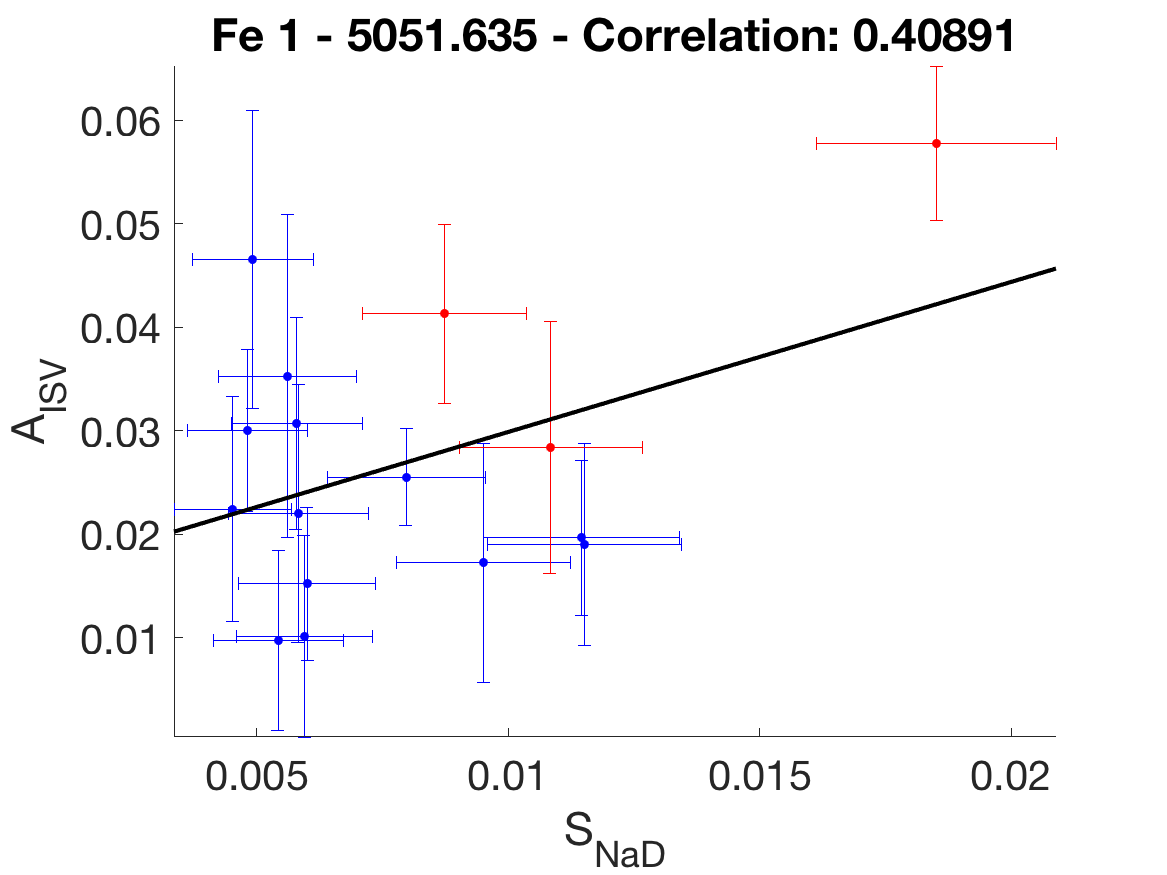
\includegraphics[width=0.5\textwidth]{CorrPlots/NaD_20.png}}\\
    \caption{}
    \label{figCorr5}
\end{figure}

\begin{figure}[!h]
    \centering
	\captionsetup{width=.8\textwidth}
    \subfloat[]{\label{figCa21}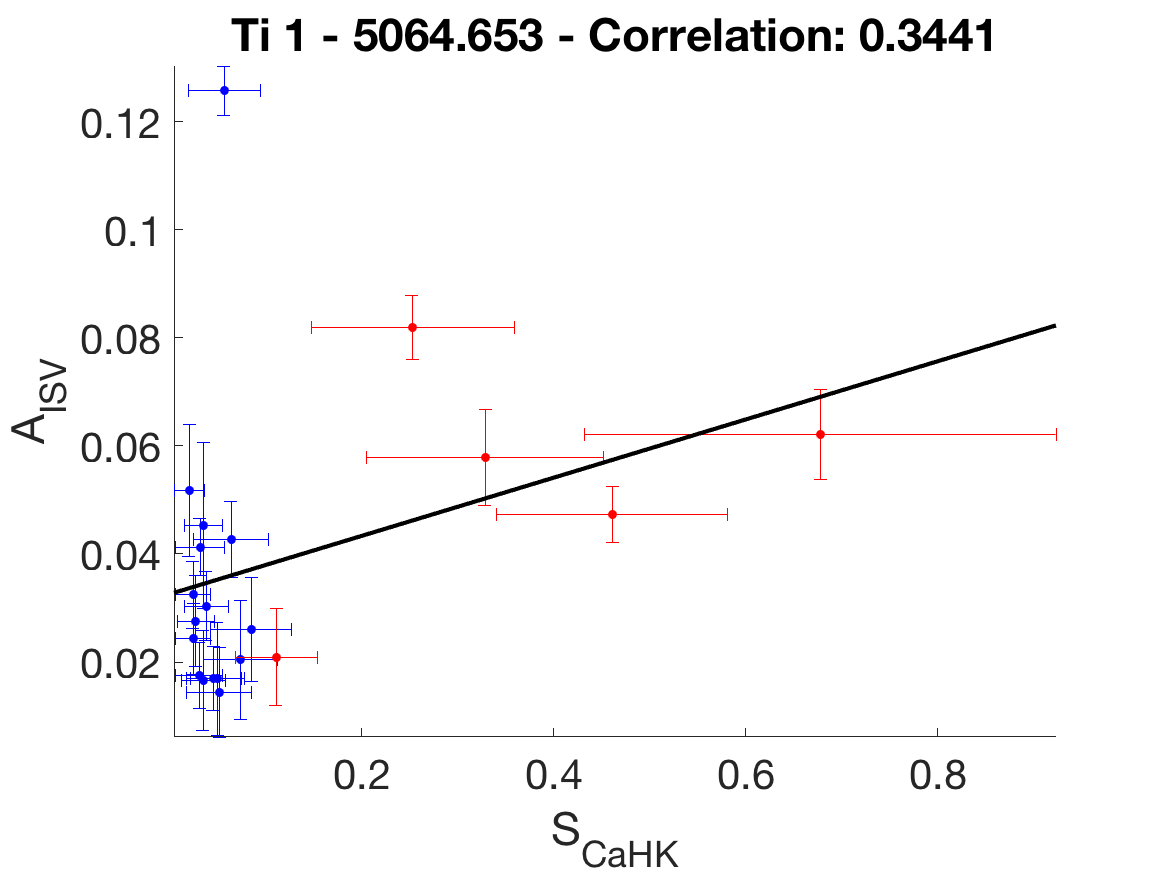
\includegraphics[width=0.5\textwidth]{CorrPlots/CaHK_21.png}}
    \subfloat[]{\label{figCa24}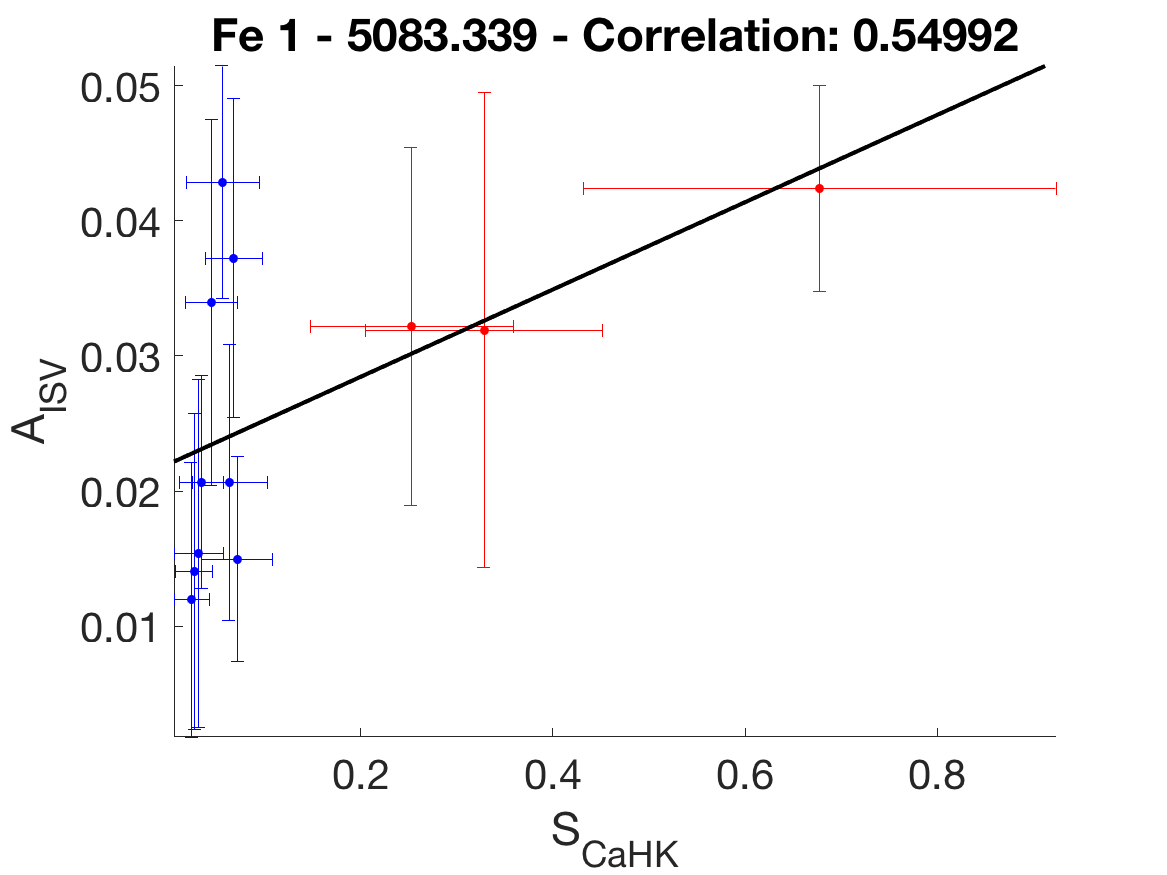
\includegraphics[width=0.5\textwidth]{CorrPlots/CaHK_24.png}}\\
    \subfloat[]{\label{figHa21}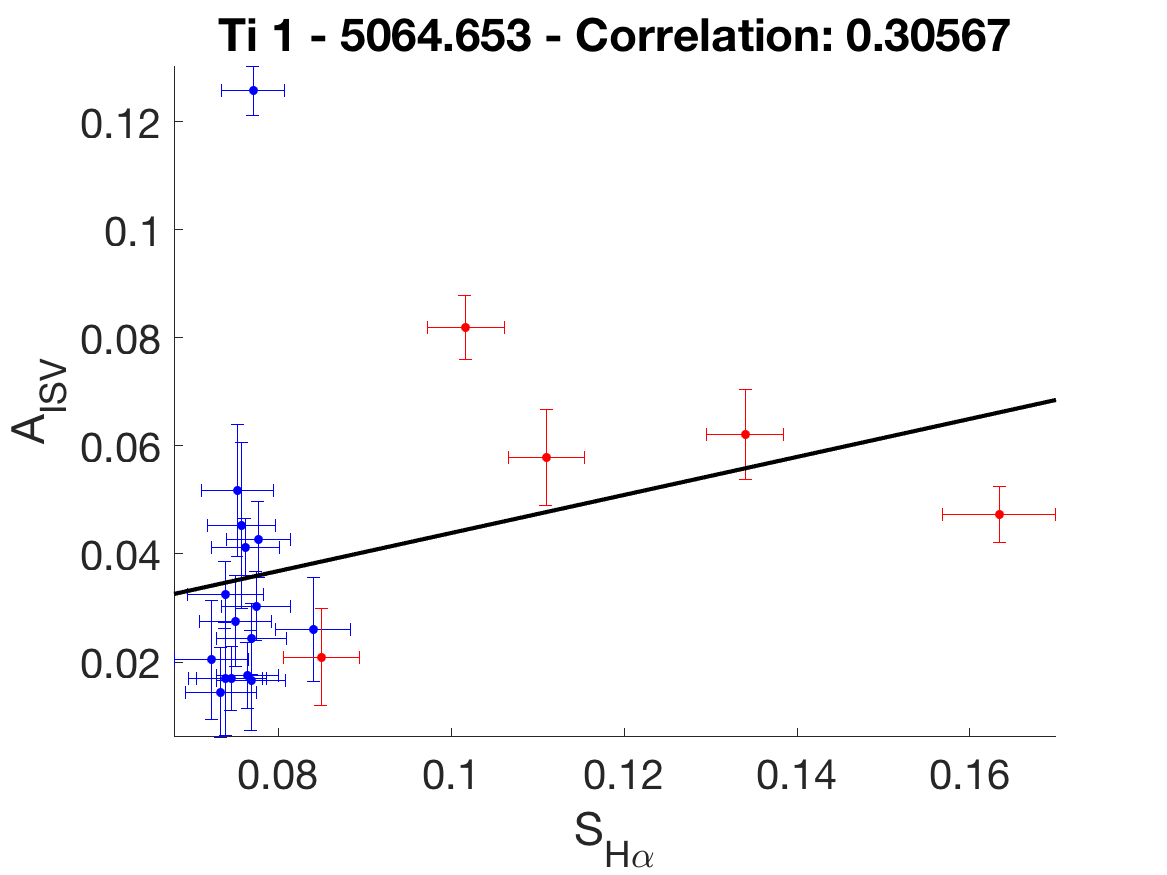
\includegraphics[width=0.5\textwidth]{CorrPlots/Halpha_21.png}}
    \subfloat[]{\label{figHa24}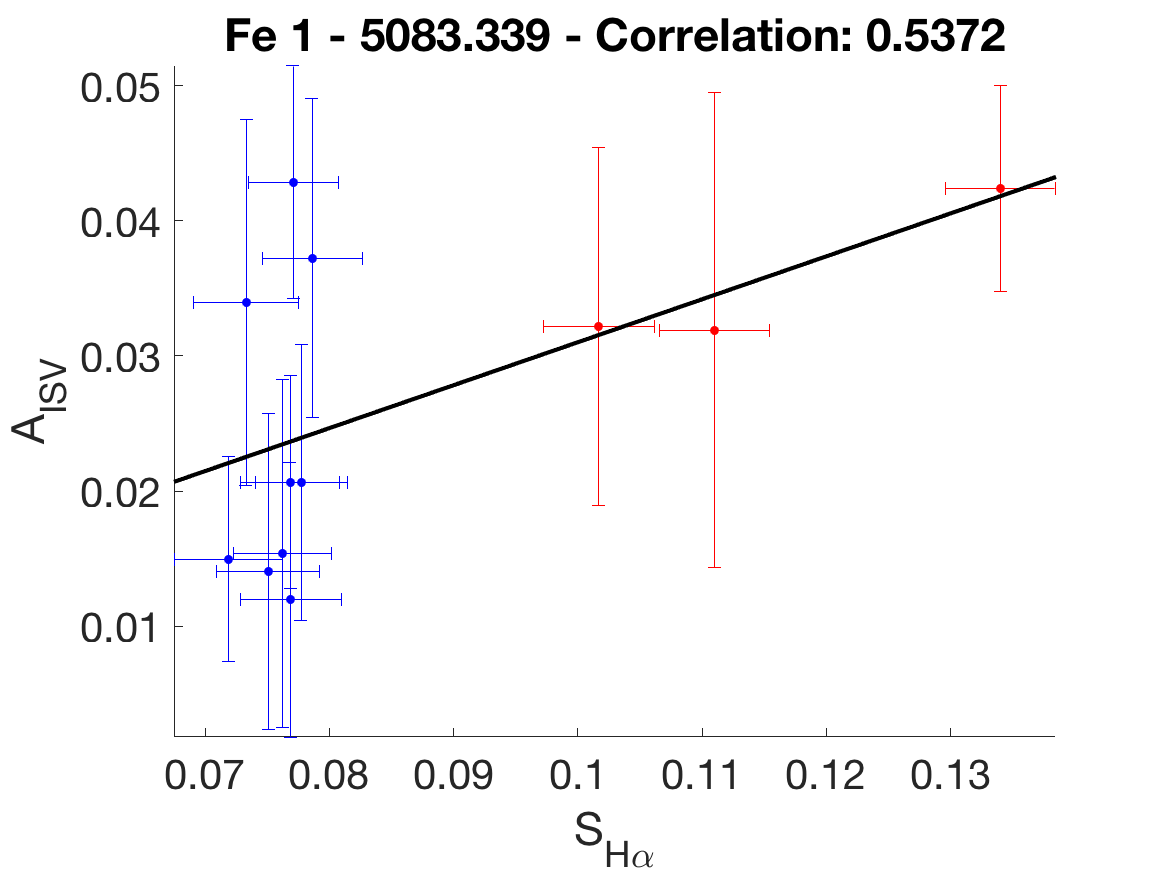
\includegraphics[width=0.5\textwidth]{CorrPlots/Halpha_24.png}}\\
    \subfloat[]{\label{figNa21}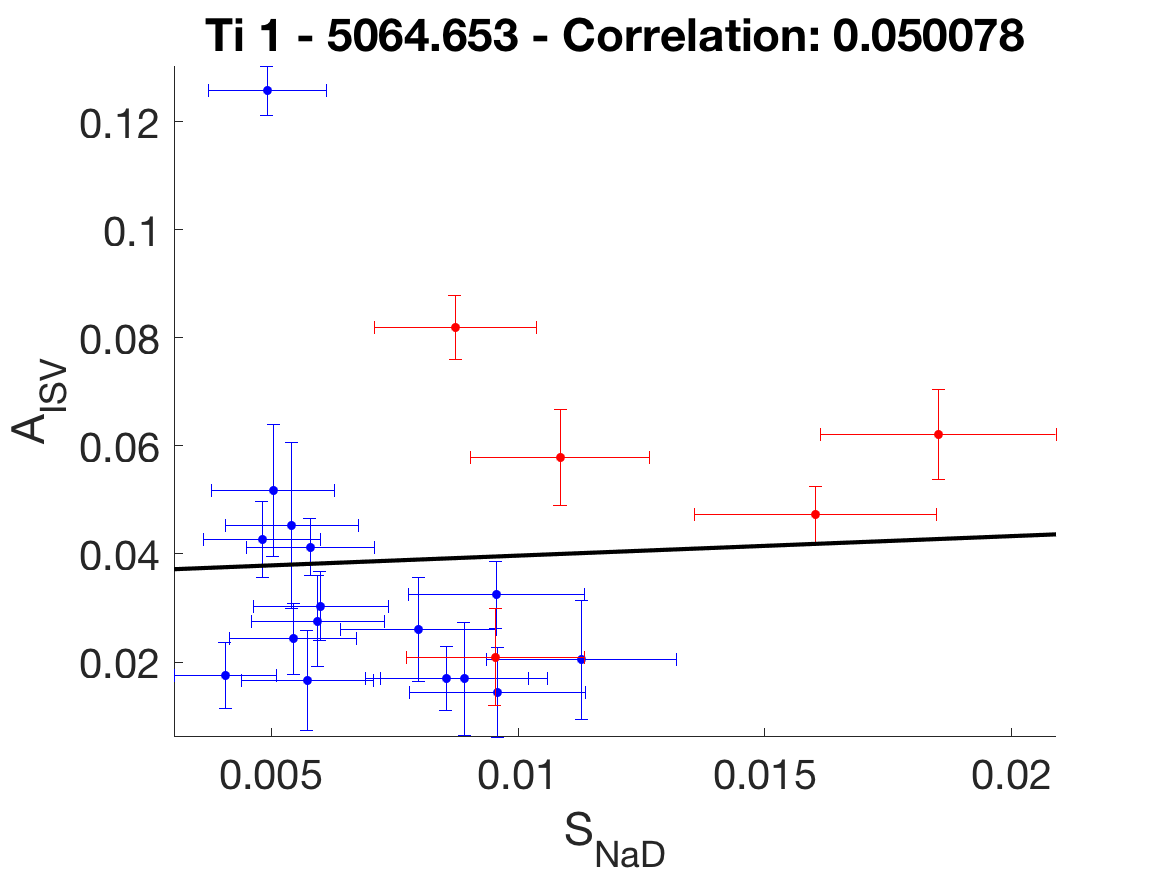
\includegraphics[width=0.5\textwidth]{CorrPlots/NaD_21.png}}
    \subfloat[]{\label{figNa24}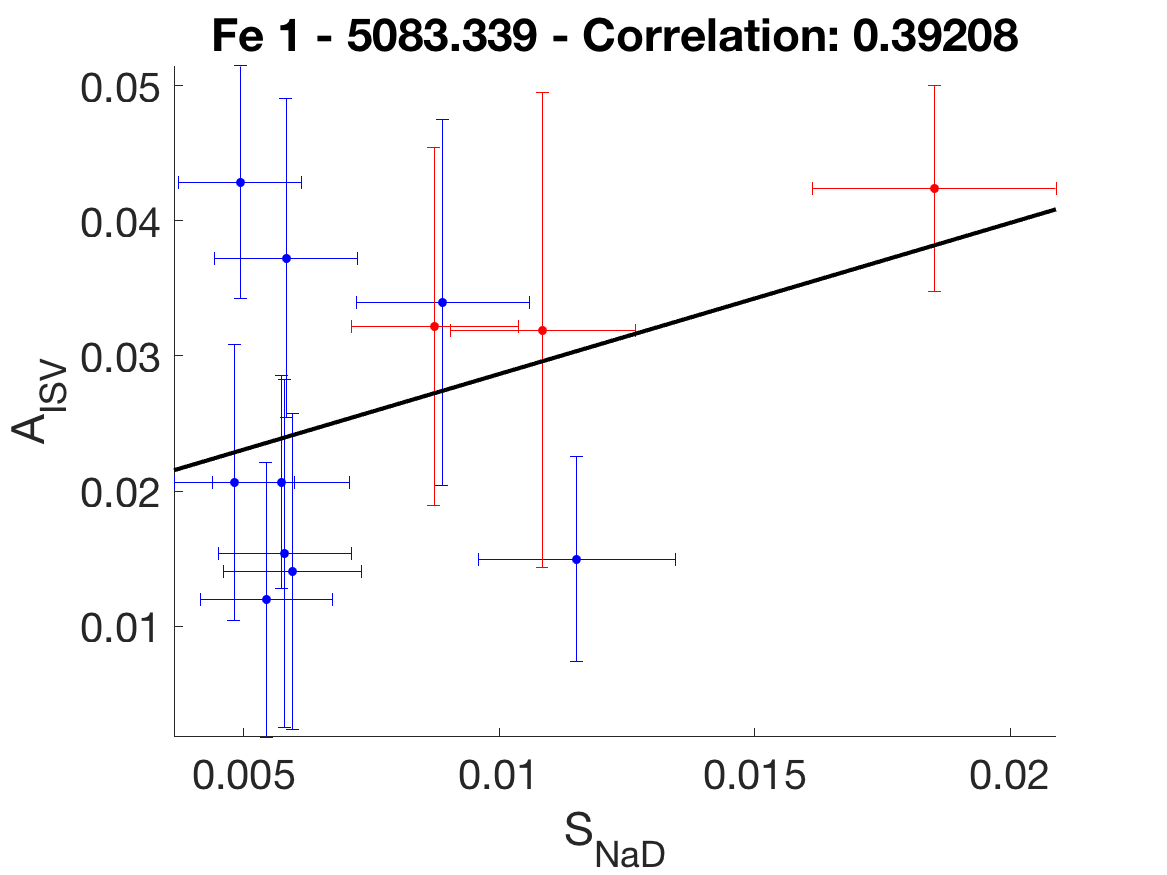
\includegraphics[width=0.5\textwidth]{CorrPlots/NaD_24.png}}\\
    \caption{}
    \label{figCorr6}
\end{figure}

\begin{figure}[!h]
    \centering
	\captionsetup{width=.8\textwidth}
    \subfloat[]{\label{figCa25}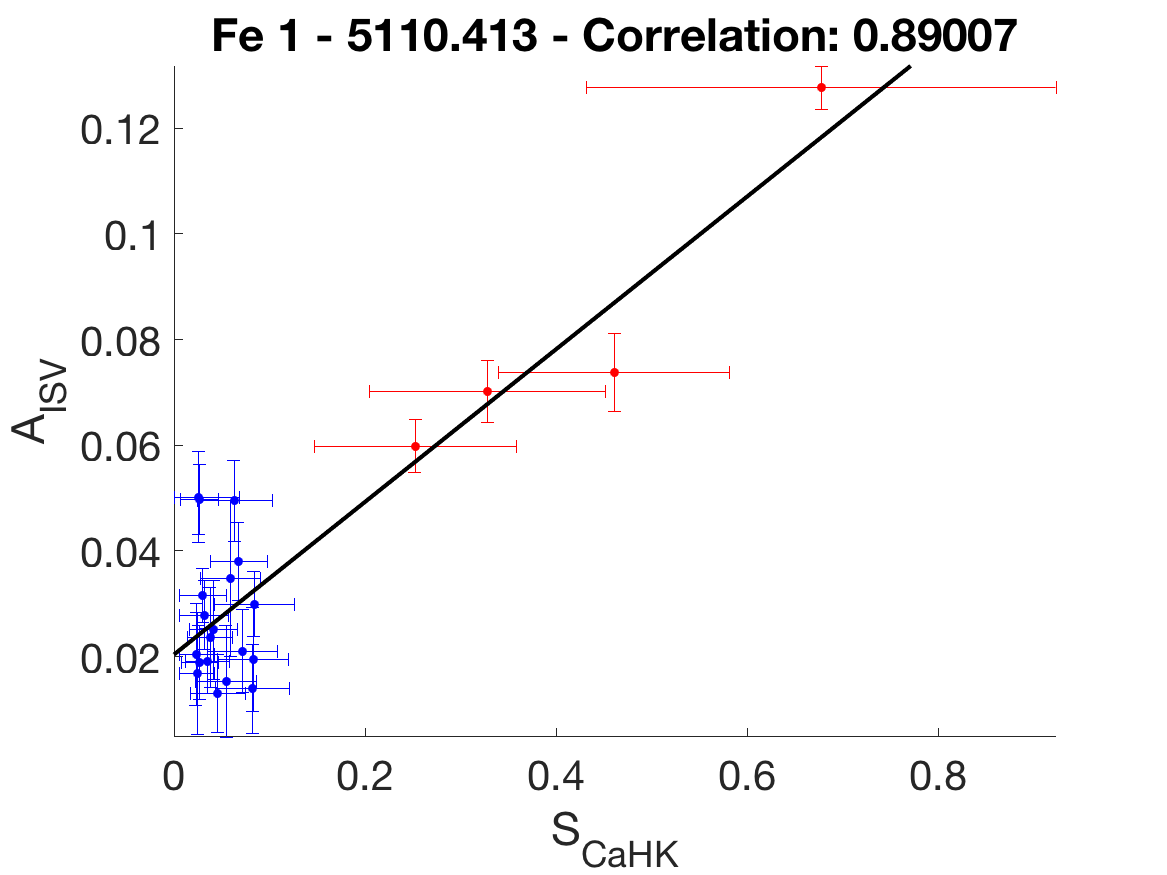
\includegraphics[width=0.5\textwidth]{CorrPlots/CaHK_25.png}}
    \subfloat[]{\label{figCa33}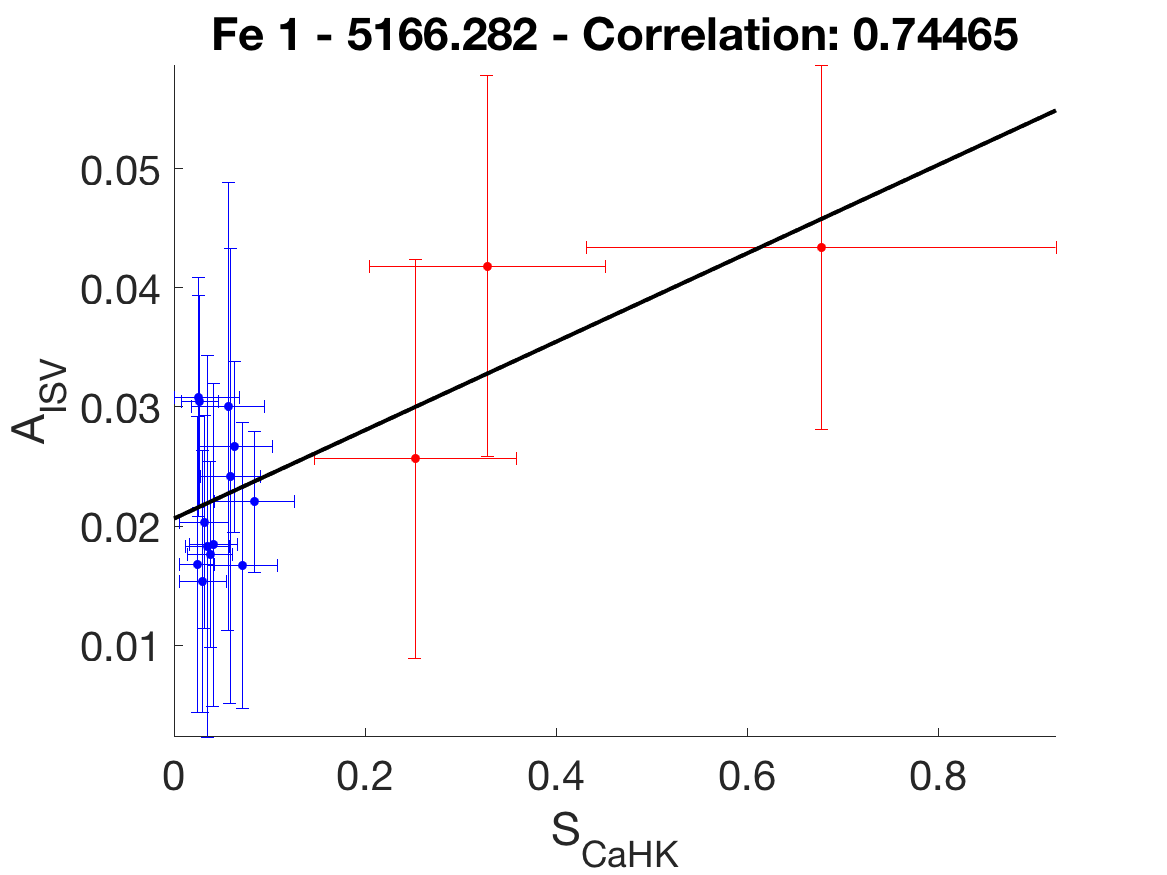
\includegraphics[width=0.5\textwidth]{CorrPlots/CaHK_33.png}}\\
    \subfloat[]{\label{figHa25}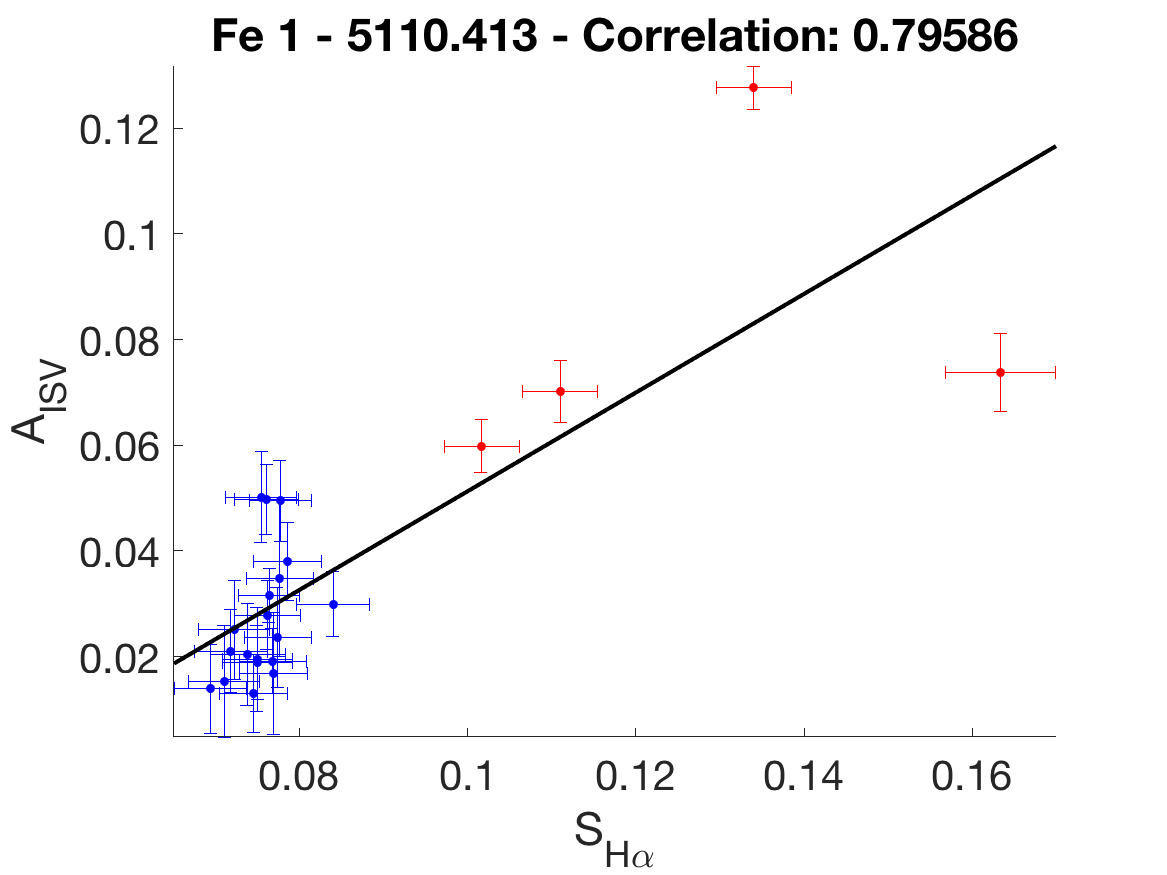
\includegraphics[width=0.5\textwidth]{CorrPlots/Halpha_25.png}}
    \subfloat[]{\label{figHa33}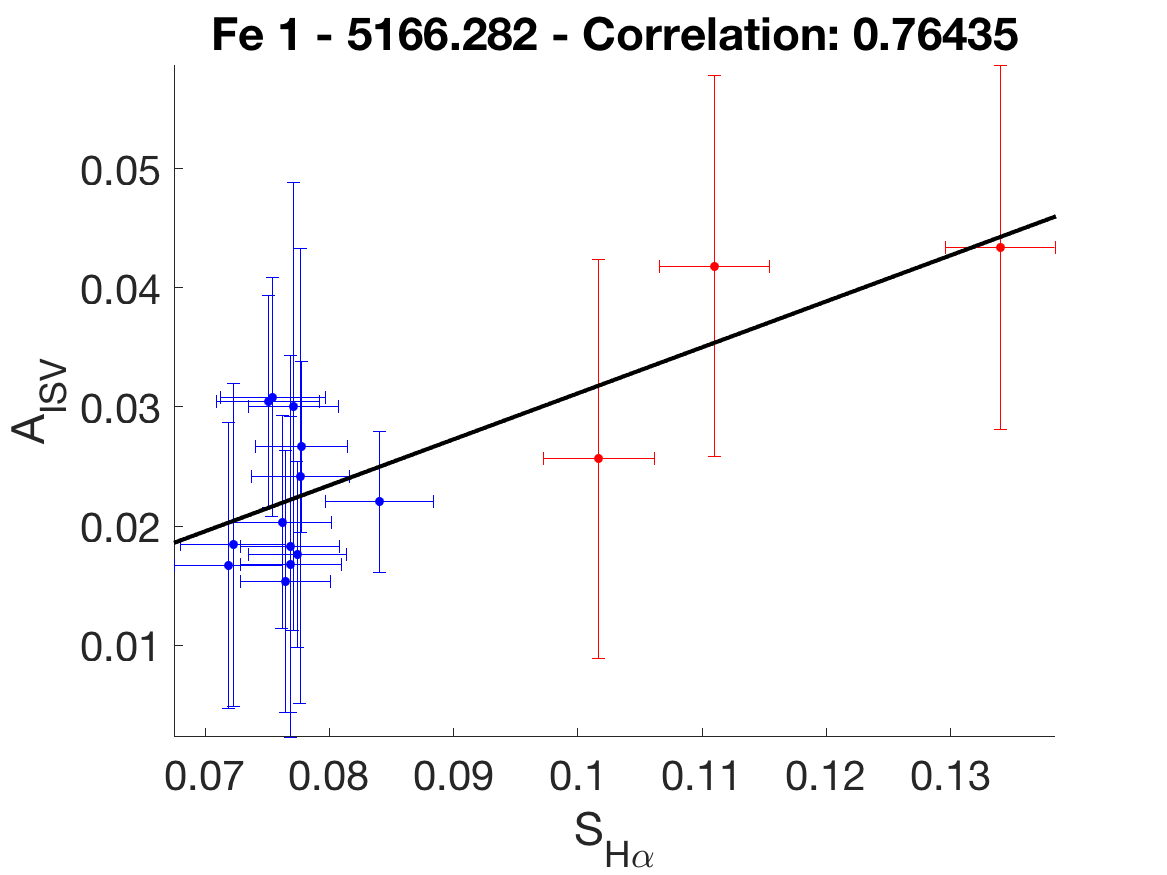
\includegraphics[width=0.5\textwidth]{CorrPlots/Halpha_33.png}}\\
    \subfloat[]{\label{figNa25}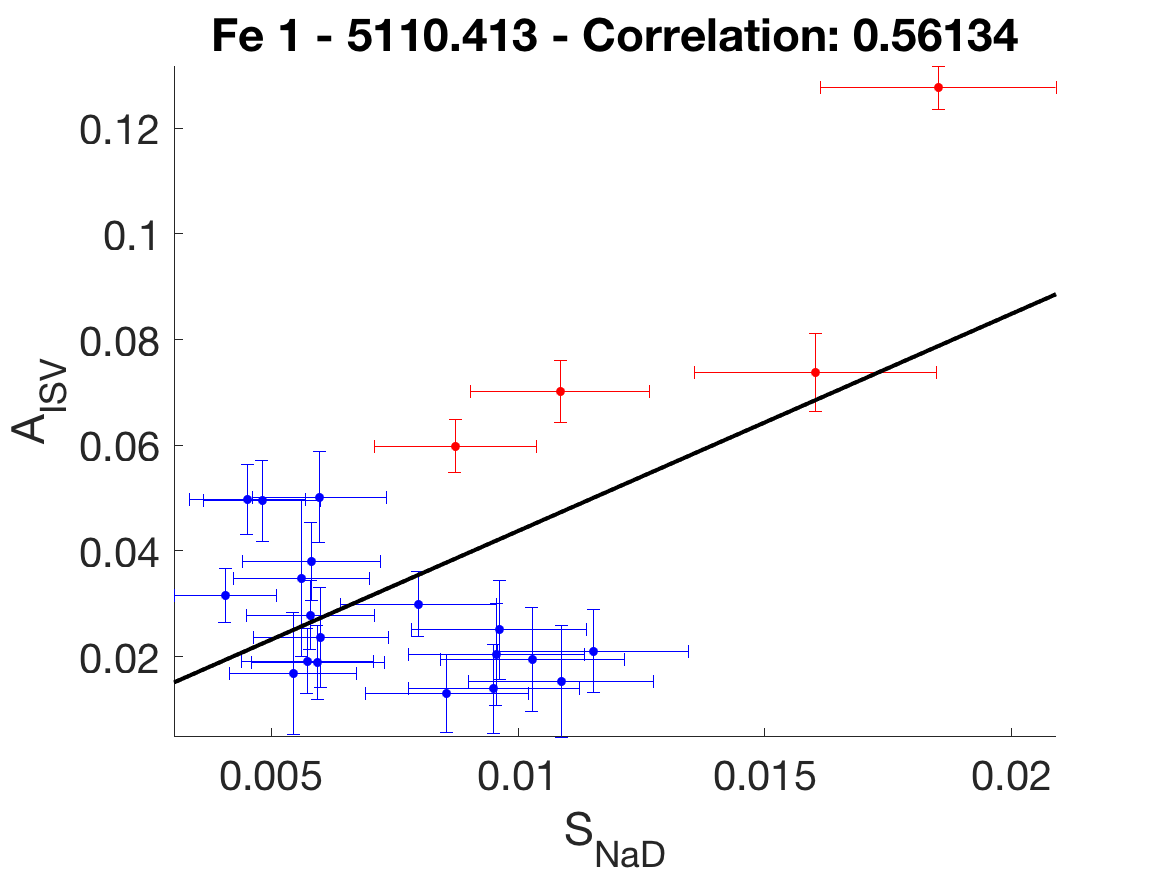
\includegraphics[width=0.5\textwidth]{CorrPlots/NaD_25.png}}
    \subfloat[]{\label{figNa33}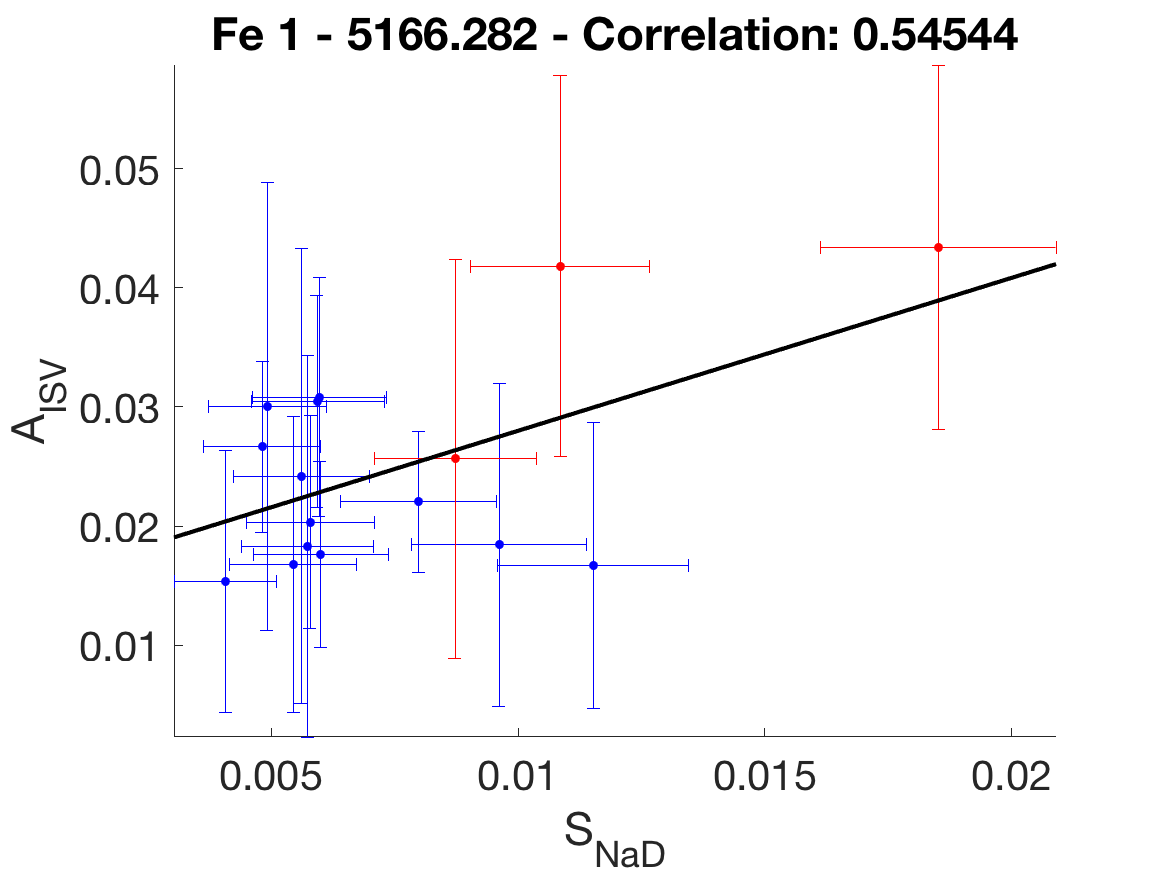
\includegraphics[width=0.5\textwidth]{CorrPlots/NaD_33.png}}\\
    \caption{}
    \label{figCorr7}
\end{figure}

\begin{figure}[!h]
    \centering
	\captionsetup{width=.8\textwidth}
    \subfloat[]{\label{figCa34}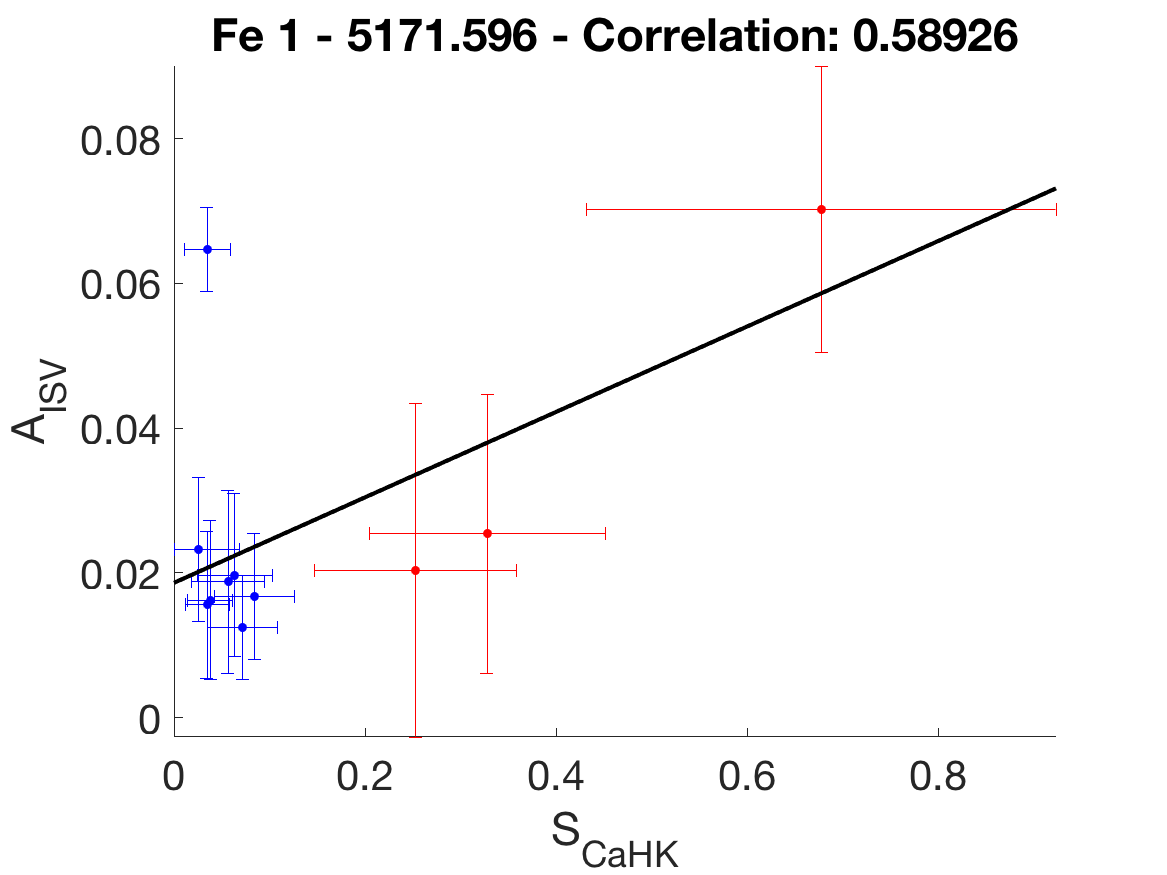
\includegraphics[width=0.5\textwidth]{CorrPlots/CaHK_34.png}}
    \subfloat[]{\label{figCa35}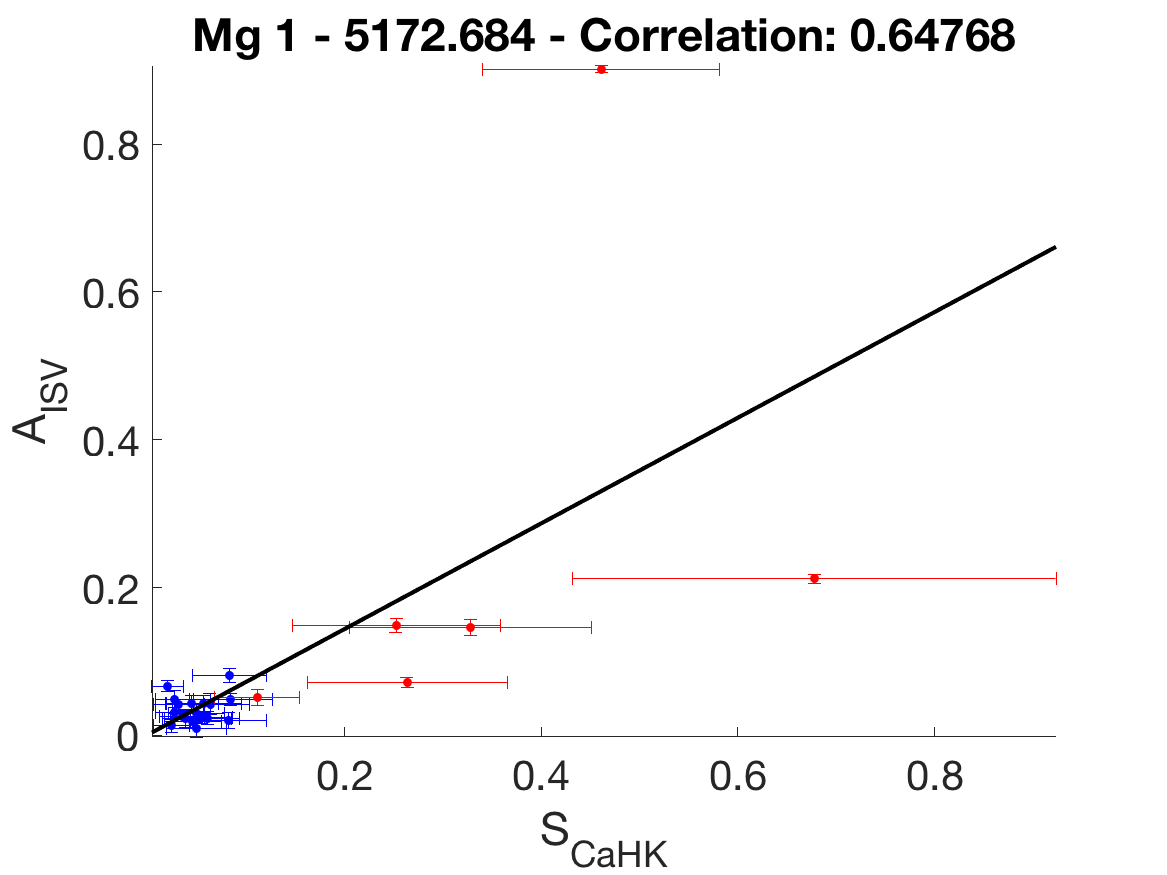
\includegraphics[width=0.5\textwidth]{CorrPlots/CaHK_35.png}}\\
    \subfloat[]{\label{figHa34}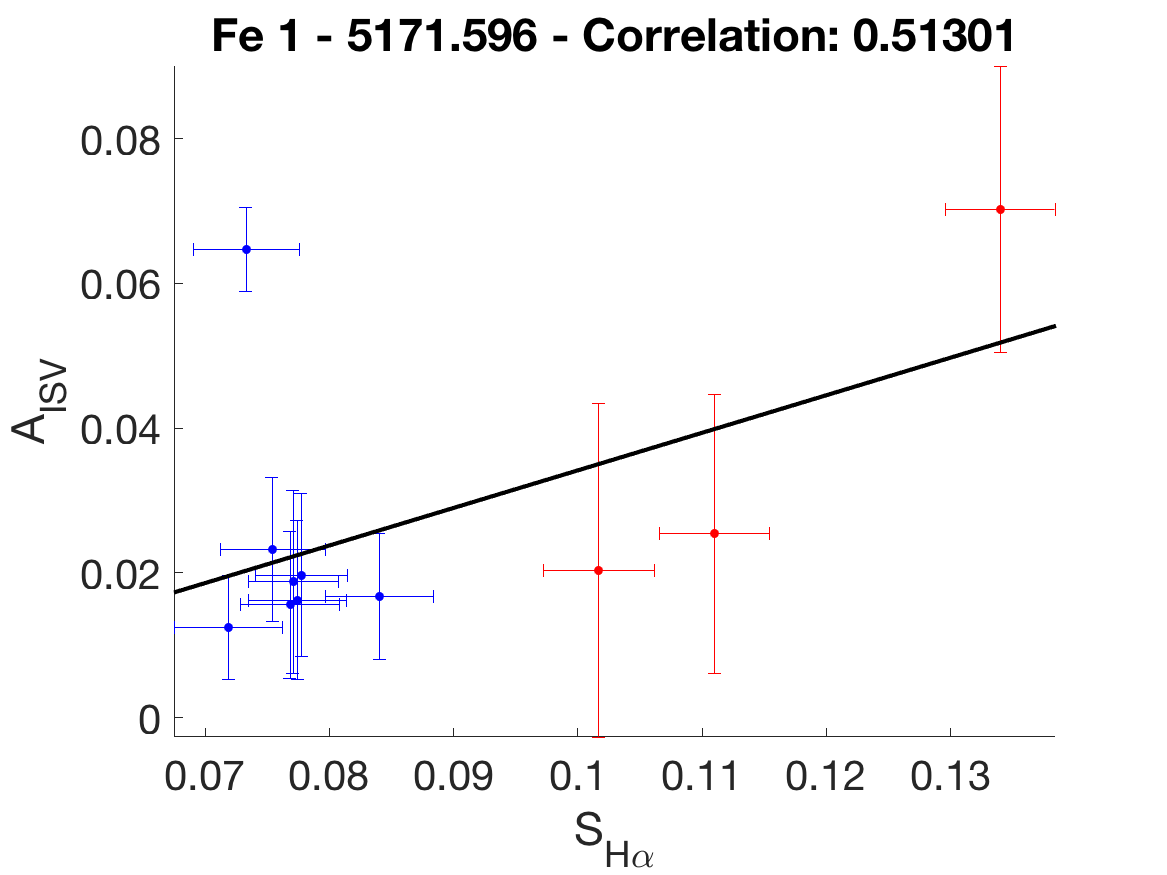
\includegraphics[width=0.5\textwidth]{CorrPlots/Halpha_34.png}}
    \subfloat[]{\label{figHa35}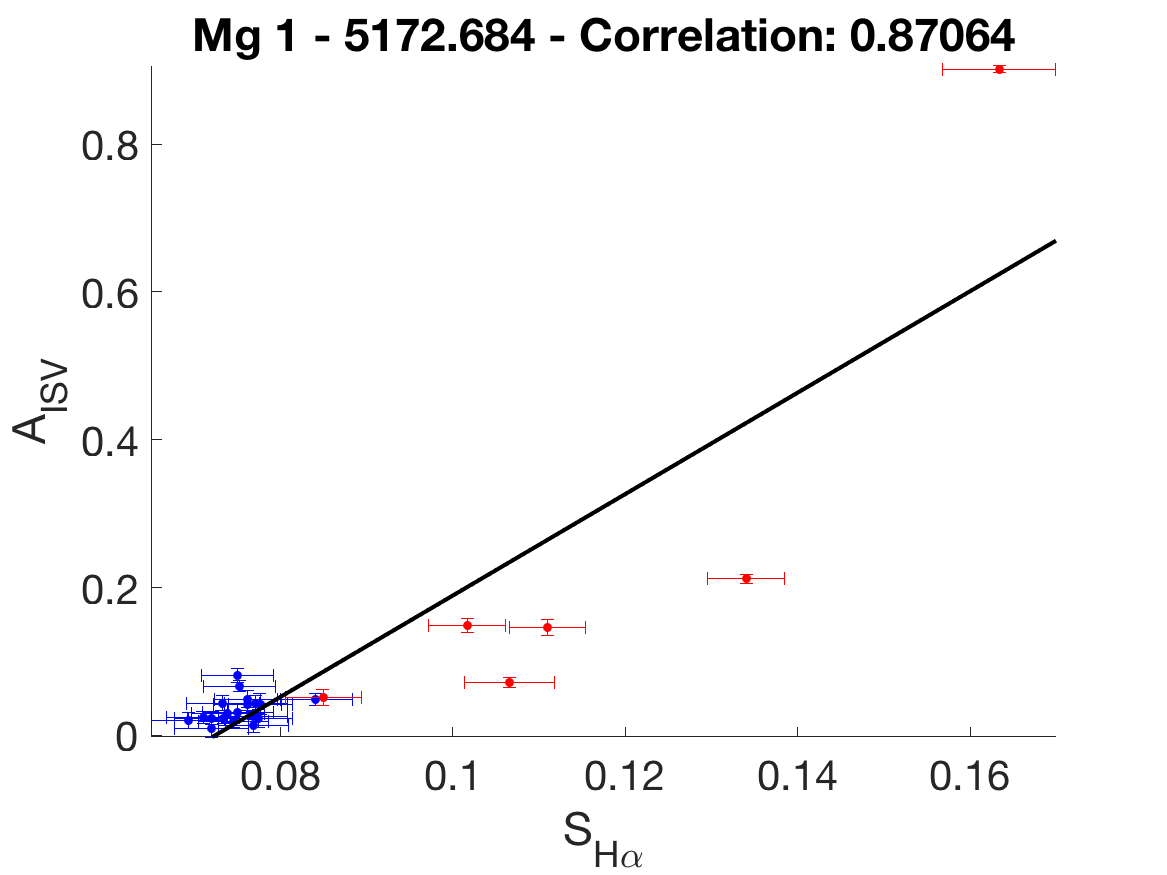
\includegraphics[width=0.5\textwidth]{CorrPlots/Halpha_35.png}}\\
    \subfloat[]{\label{figNa34}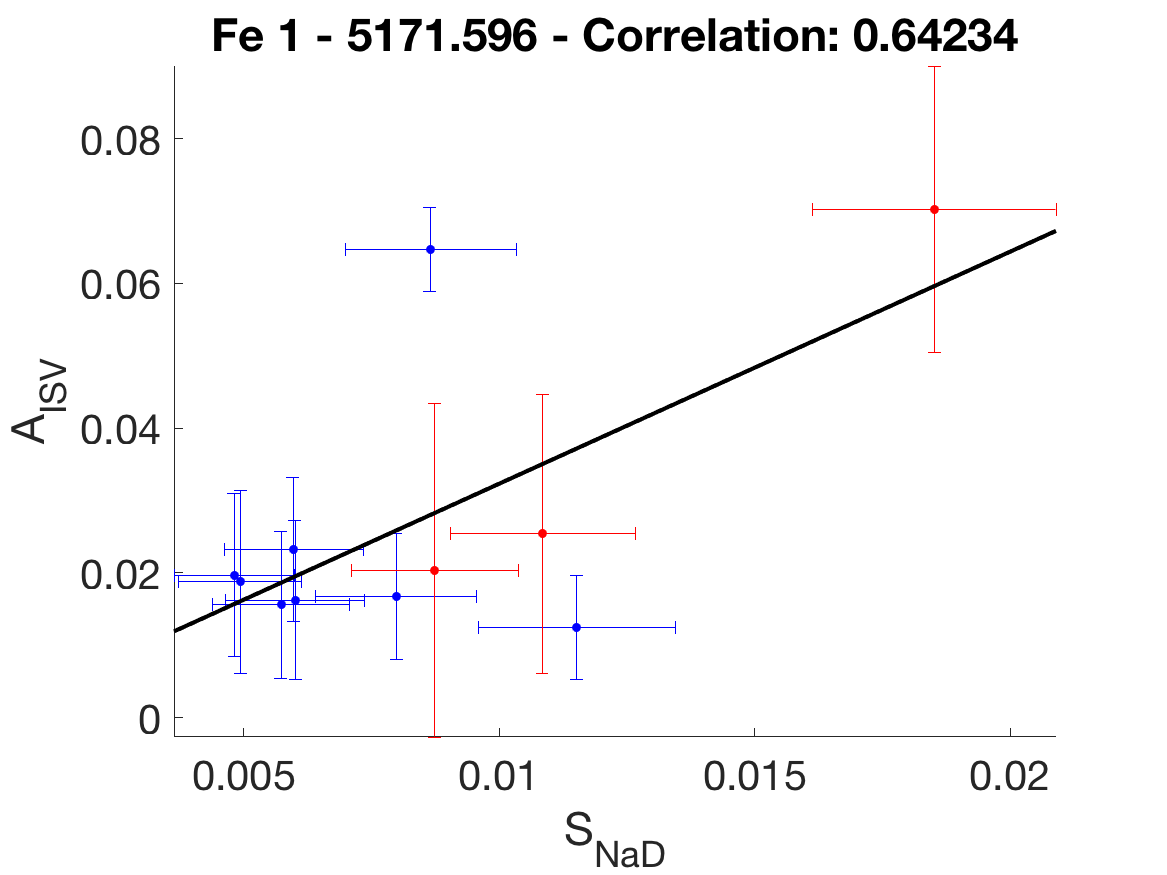
\includegraphics[width=0.5\textwidth]{CorrPlots/NaD_34.png}}
    \subfloat[]{\label{figNa35}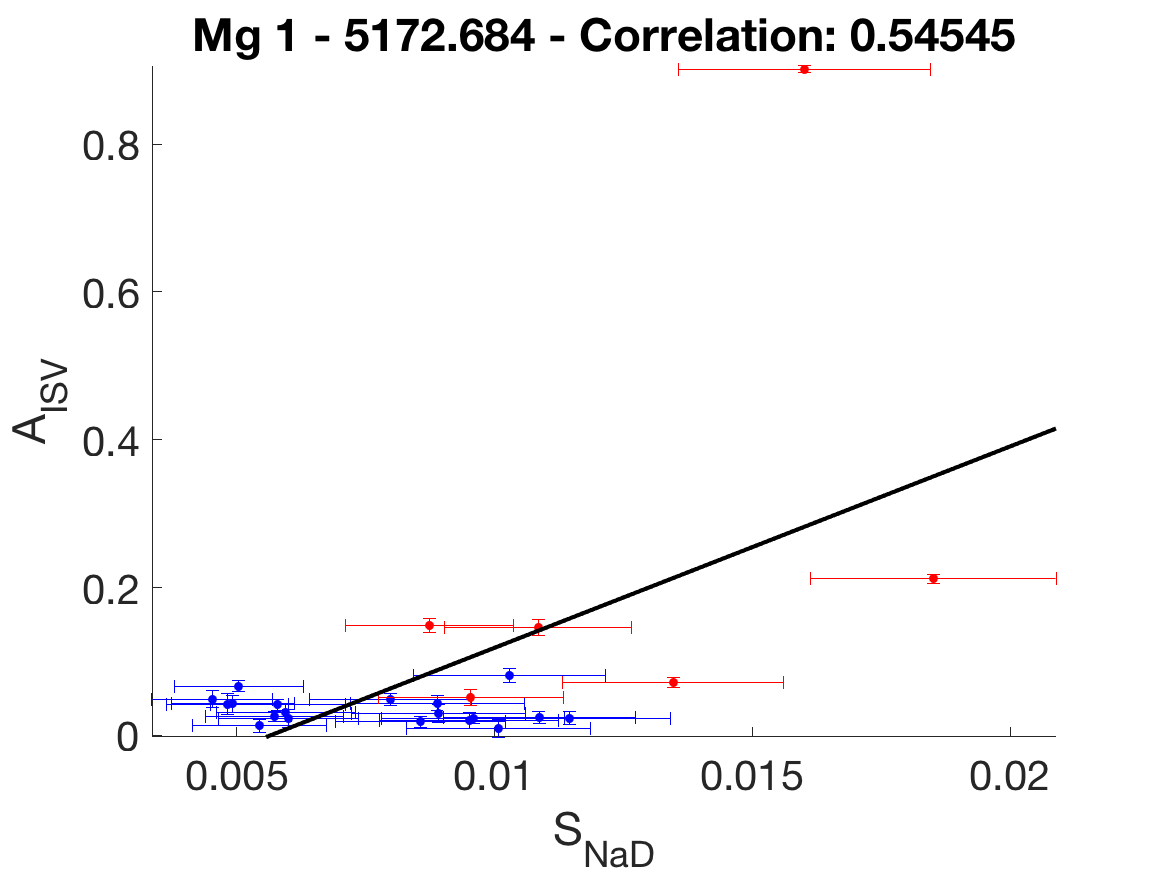
\includegraphics[width=0.5\textwidth]{CorrPlots/NaD_35.png}}\\
    \caption{}
    \label{figCorr8}
\end{figure}

\begin{figure}[!h]
    \centering
	\captionsetup{width=.8\textwidth}
    \subfloat[]{\label{figCa36}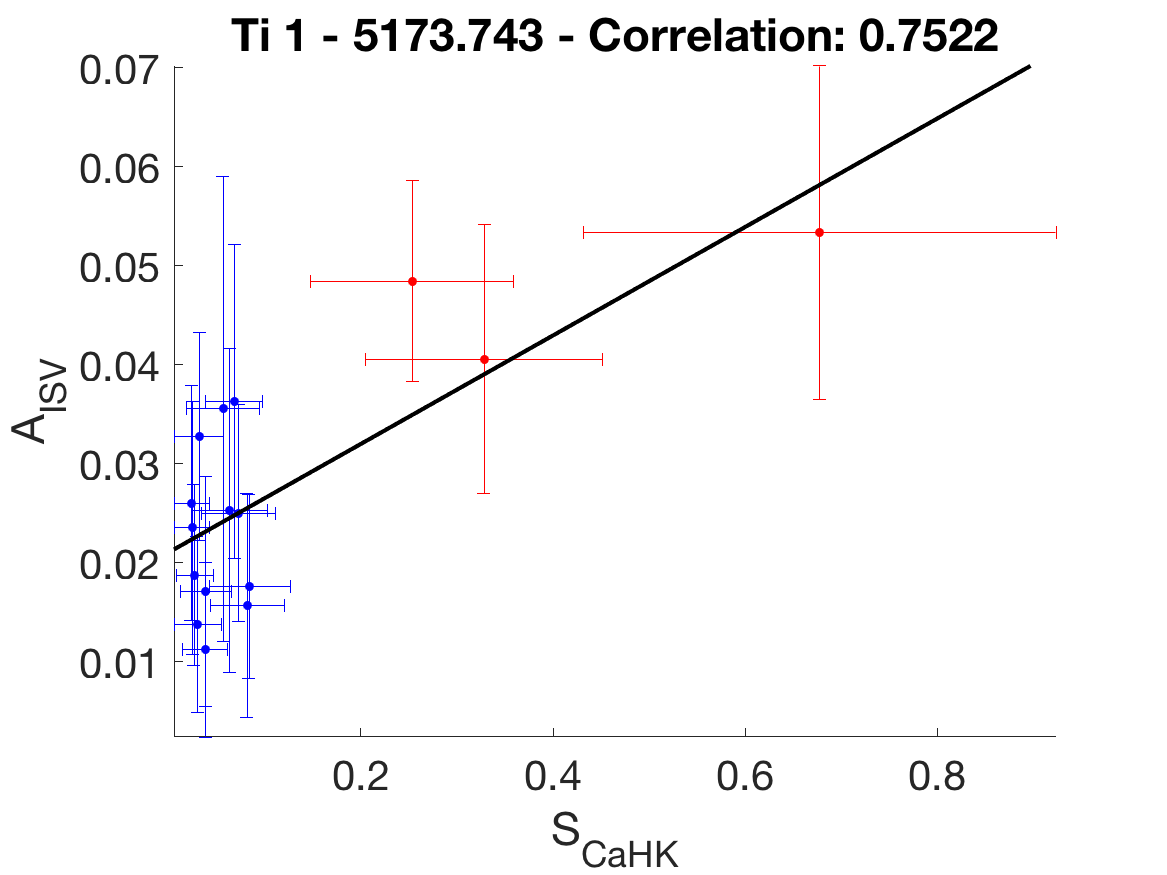
\includegraphics[width=0.5\textwidth]{CorrPlots/CaHK_36.png}}
    \subfloat[]{\label{figCa37}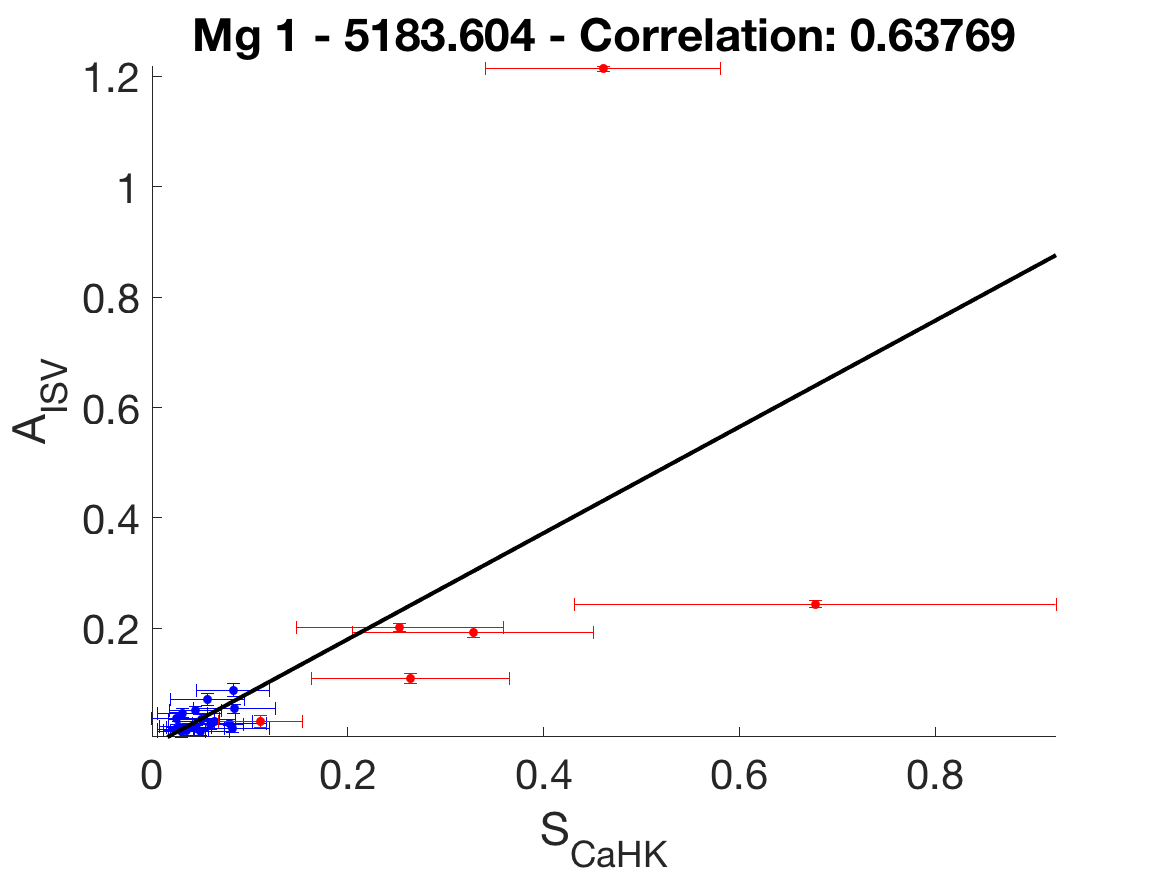
\includegraphics[width=0.5\textwidth]{CorrPlots/CaHK_37.png}}\\
    \subfloat[]{\label{figHa36}\includegraphics[width=0.5\textwidth]{CorrPlots/Halpha_36.png}}
    \subfloat[]{\label{figHa37}\includegraphics[width=0.5\textwidth]{CorrPlots/Halpha_37.png}}\\
    \subfloat[]{\label{figNa36}\includegraphics[width=0.5\textwidth]{CorrPlots/NaD_36.png}}
    \subfloat[]{\label{figNa37}\includegraphics[width=0.5\textwidth]{CorrPlots/NaD_37.png}}\\
    \caption{}
    \label{figCorr9}
\end{figure}

\begin{figure}[!h]
    \centering
	\captionsetup{width=.8\textwidth}
    \subfloat[]{\label{figCa38}\includegraphics[width=0.5\textwidth]{CorrPlots/CaHK_38.png}}
    \subfloat[]{\label{figCa42}\includegraphics[width=0.5\textwidth]{CorrPlots/CaHK_42.png}}\\
    \subfloat[]{\label{figHa38}\includegraphics[width=0.5\textwidth]{CorrPlots/Halpha_38.png}}
    \subfloat[]{\label{figHa42}\includegraphics[width=0.5\textwidth]{CorrPlots/Halpha_42.png}}\\
    \subfloat[]{\label{figNa38}\includegraphics[width=0.5\textwidth]{CorrPlots/NaD_38.png}}
    \subfloat[]{\label{figNa42}\includegraphics[width=0.5\textwidth]{CorrPlots/NaD_42.png}}\\
    \caption{}
    \label{figCorr10}
\end{figure}

\begin{figure}[!h]
    \centering
	\captionsetup{width=.8\textwidth}
    \subfloat[]{\label{figCa43}\includegraphics[width=0.5\textwidth]{CorrPlots/CaHK_43.png}}
    \subfloat[]{\label{figCa46}\includegraphics[width=0.5\textwidth]{CorrPlots/CaHK_46.png}}\\
    \subfloat[]{\label{figHa43}\includegraphics[width=0.5\textwidth]{CorrPlots/Halpha_43.png}}
    \subfloat[]{\label{figHa46}\includegraphics[width=0.5\textwidth]{CorrPlots/Halpha_46.png}}\\
    \subfloat[]{\label{figNa43}\includegraphics[width=0.5\textwidth]{CorrPlots/NaD_43.png}}
    \subfloat[]{\label{figNa46}\includegraphics[width=0.5\textwidth]{CorrPlots/NaD_46.png}}\\
    \caption{}
    \label{figCorr11}
\end{figure}

\begin{figure}[!h]
    \centering
	\captionsetup{width=.8\textwidth}
    \subfloat[]{\label{figCa47}\includegraphics[width=0.5\textwidth]{CorrPlots/CaHK_47.png}}
    \subfloat[]{\label{figCa51}\includegraphics[width=0.5\textwidth]{CorrPlots/CaHK_51.png}}\\
    \subfloat[]{\label{figHa47}\includegraphics[width=0.5\textwidth]{CorrPlots/Halpha_47.png}}
    \subfloat[]{\label{figHa51}\includegraphics[width=0.5\textwidth]{CorrPlots/Halpha_51.png}}\\
    \subfloat[]{\label{figNa47}\includegraphics[width=0.5\textwidth]{CorrPlots/NaD_47.png}}
    \subfloat[]{\label{figNa51}\includegraphics[width=0.5\textwidth]{CorrPlots/NaD_51.png}}\\
    \caption{}
    \label{figCorr12}
\end{figure}

\begin{figure}[!h]
    \centering
	\captionsetup{width=.8\textwidth}
    \subfloat[]{\label{figCa54}\includegraphics[width=0.5\textwidth]{CorrPlots/CaHK_54.png}}
    \subfloat[]{\label{figCa55}\includegraphics[width=0.5\textwidth]{CorrPlots/CaHK_55.png}}\\
    \subfloat[]{\label{figHa54}\includegraphics[width=0.5\textwidth]{CorrPlots/Halpha_54.png}}
    \subfloat[]{\label{figHa55}\includegraphics[width=0.5\textwidth]{CorrPlots/Halpha_55.png}}\\
    \subfloat[]{\label{figNa54}\includegraphics[width=0.5\textwidth]{CorrPlots/NaD_54.png}}
    \subfloat[]{\label{figNa55}\includegraphics[width=0.5\textwidth]{CorrPlots/NaD_55.png}}\\
    \caption{}
    \label{figCorr13}
\end{figure}

\begin{figure}[!h]
    \centering
	\captionsetup{width=.8\textwidth}
    \subfloat[]{\label{figCa57}\includegraphics[width=0.5\textwidth]{CorrPlots/CaHK_57.png}}
    \subfloat[]{\label{figCa58}\includegraphics[width=0.5\textwidth]{CorrPlots/CaHK_58.png}}\\
    \subfloat[]{\label{figHa57}\includegraphics[width=0.5\textwidth]{CorrPlots/Halpha_57.png}}
    \subfloat[]{\label{figHa58}\includegraphics[width=0.5\textwidth]{CorrPlots/Halpha_58.png}}\\
    \subfloat[]{\label{figNa57}\includegraphics[width=0.5\textwidth]{CorrPlots/NaD_57.png}}
    \subfloat[]{\label{figNa58}\includegraphics[width=0.5\textwidth]{CorrPlots/NaD_58.png}}\\
    \caption{}
    \label{figCorr14}
\end{figure}

\begin{figure}[!h]
    \centering
	\captionsetup{width=.8\textwidth}
    \subfloat[]{\label{figCa59}\includegraphics[width=0.5\textwidth]{CorrPlots/CaHK_59.png}}
    \subfloat[]{\label{figCa60}\includegraphics[width=0.5\textwidth]{CorrPlots/CaHK_60.png}}\\
    \subfloat[]{\label{figHa59}\includegraphics[width=0.5\textwidth]{CorrPlots/Halpha_59.png}}
    \subfloat[]{\label{figHa60}\includegraphics[width=0.5\textwidth]{CorrPlots/Halpha_60.png}}\\
    \subfloat[]{\label{figNa59}\includegraphics[width=0.5\textwidth]{CorrPlots/NaD_59.png}}
    \subfloat[]{\label{figNa60}\includegraphics[width=0.5\textwidth]{CorrPlots/NaD_60.png}}\\
    \caption{}
    \label{figCorr15}
\end{figure}

\begin{figure}[!h]
    \centering
	\captionsetup{width=.8\textwidth}
    \subfloat[]{\label{figCa61}\includegraphics[width=0.5\textwidth]{CorrPlots/CaHK_61.png}}
    \subfloat[]{\label{figCa62}\includegraphics[width=0.5\textwidth]{CorrPlots/CaHK_62.png}}\\
    \subfloat[]{\label{figHa61}\includegraphics[width=0.5\textwidth]{CorrPlots/Halpha_61.png}}
    \subfloat[]{\label{figHa62}\includegraphics[width=0.5\textwidth]{CorrPlots/Halpha_62.png}}\\
    \subfloat[]{\label{figNa61}\includegraphics[width=0.5\textwidth]{CorrPlots/NaD_61.png}}
    \subfloat[]{\label{figNa62}\includegraphics[width=0.5\textwidth]{CorrPlots/NaD_62.png}}\\
    \caption{}
    \label{figCorr16}
\end{figure}

\begin{figure}[!h]
    \centering
	\captionsetup{width=.8\textwidth}
    \subfloat[]{\label{figCa63}\includegraphics[width=0.5\textwidth]{CorrPlots/CaHK_63.png}}
    \subfloat[]{\label{figCa64}\includegraphics[width=0.5\textwidth]{CorrPlots/CaHK_64.png}}\\
    \subfloat[]{\label{figHa63}\includegraphics[width=0.5\textwidth]{CorrPlots/Halpha_63.png}}
    \subfloat[]{\label{figHa64}\includegraphics[width=0.5\textwidth]{CorrPlots/Halpha_64.png}}\\
    \subfloat[]{\label{figNa63}\includegraphics[width=0.5\textwidth]{CorrPlots/NaD_63.png}}
    \subfloat[]{\label{figNa64}\includegraphics[width=0.5\textwidth]{CorrPlots/NaD_64.png}}\\
    \caption{}
    \label{figCorr17}
\end{figure}

\begin{figure}[!h]
    \centering
	\captionsetup{width=.8\textwidth}
    \subfloat[]{\label{figCa68}\includegraphics[width=0.5\textwidth]{CorrPlots/CaHK_68.png}}
    \subfloat[]{\label{figCa90}\includegraphics[width=0.5\textwidth]{CorrPlots/CaHK_90.png}}\\
    \subfloat[]{\label{figHa68}\includegraphics[width=0.5\textwidth]{CorrPlots/Halpha_68.png}}
    \subfloat[]{\label{figHa90}\includegraphics[width=0.5\textwidth]{CorrPlots/Halpha_90.png}}\\
    \subfloat[]{\label{figNa68}\includegraphics[width=0.5\textwidth]{CorrPlots/NaD_68.png}}
    \subfloat[]{\label{figNa90}\includegraphics[width=0.5\textwidth]{CorrPlots/NaD_90.png}}\\
    \caption{}
    \label{figCorr18}
\end{figure}

\begin{figure}[!h]
    \centering
	\captionsetup{width=.8\textwidth}
    \subfloat[]{\label{figCa91}\includegraphics[width=0.5\textwidth]{CorrPlots/CaHK_91.png}}\\
    \subfloat[]{\label{figHa91}\includegraphics[width=0.5\textwidth]{CorrPlots/Halpha_91.png}}\\
    \subfloat[]{\label{figNa91}\includegraphics[width=0.5\textwidth]{CorrPlots/NaD_91.png}}\\
    \caption{}
    \label{figCorr19}
\end{figure}

